\chapter{Graphes : méthodes et algorithmes}

\section{Niveaux dans un graphe orienté sans circuit}

On dit qu'un graphe orienté est \textit{sans circuit} lorsqu'il \dots ne comporte aucun circuit, c'est-à-dire qu'on ne peut pas trouver un chemin partant d'un sommet et y revenant.


\begin{multicols}{2}
    \begin{center}
        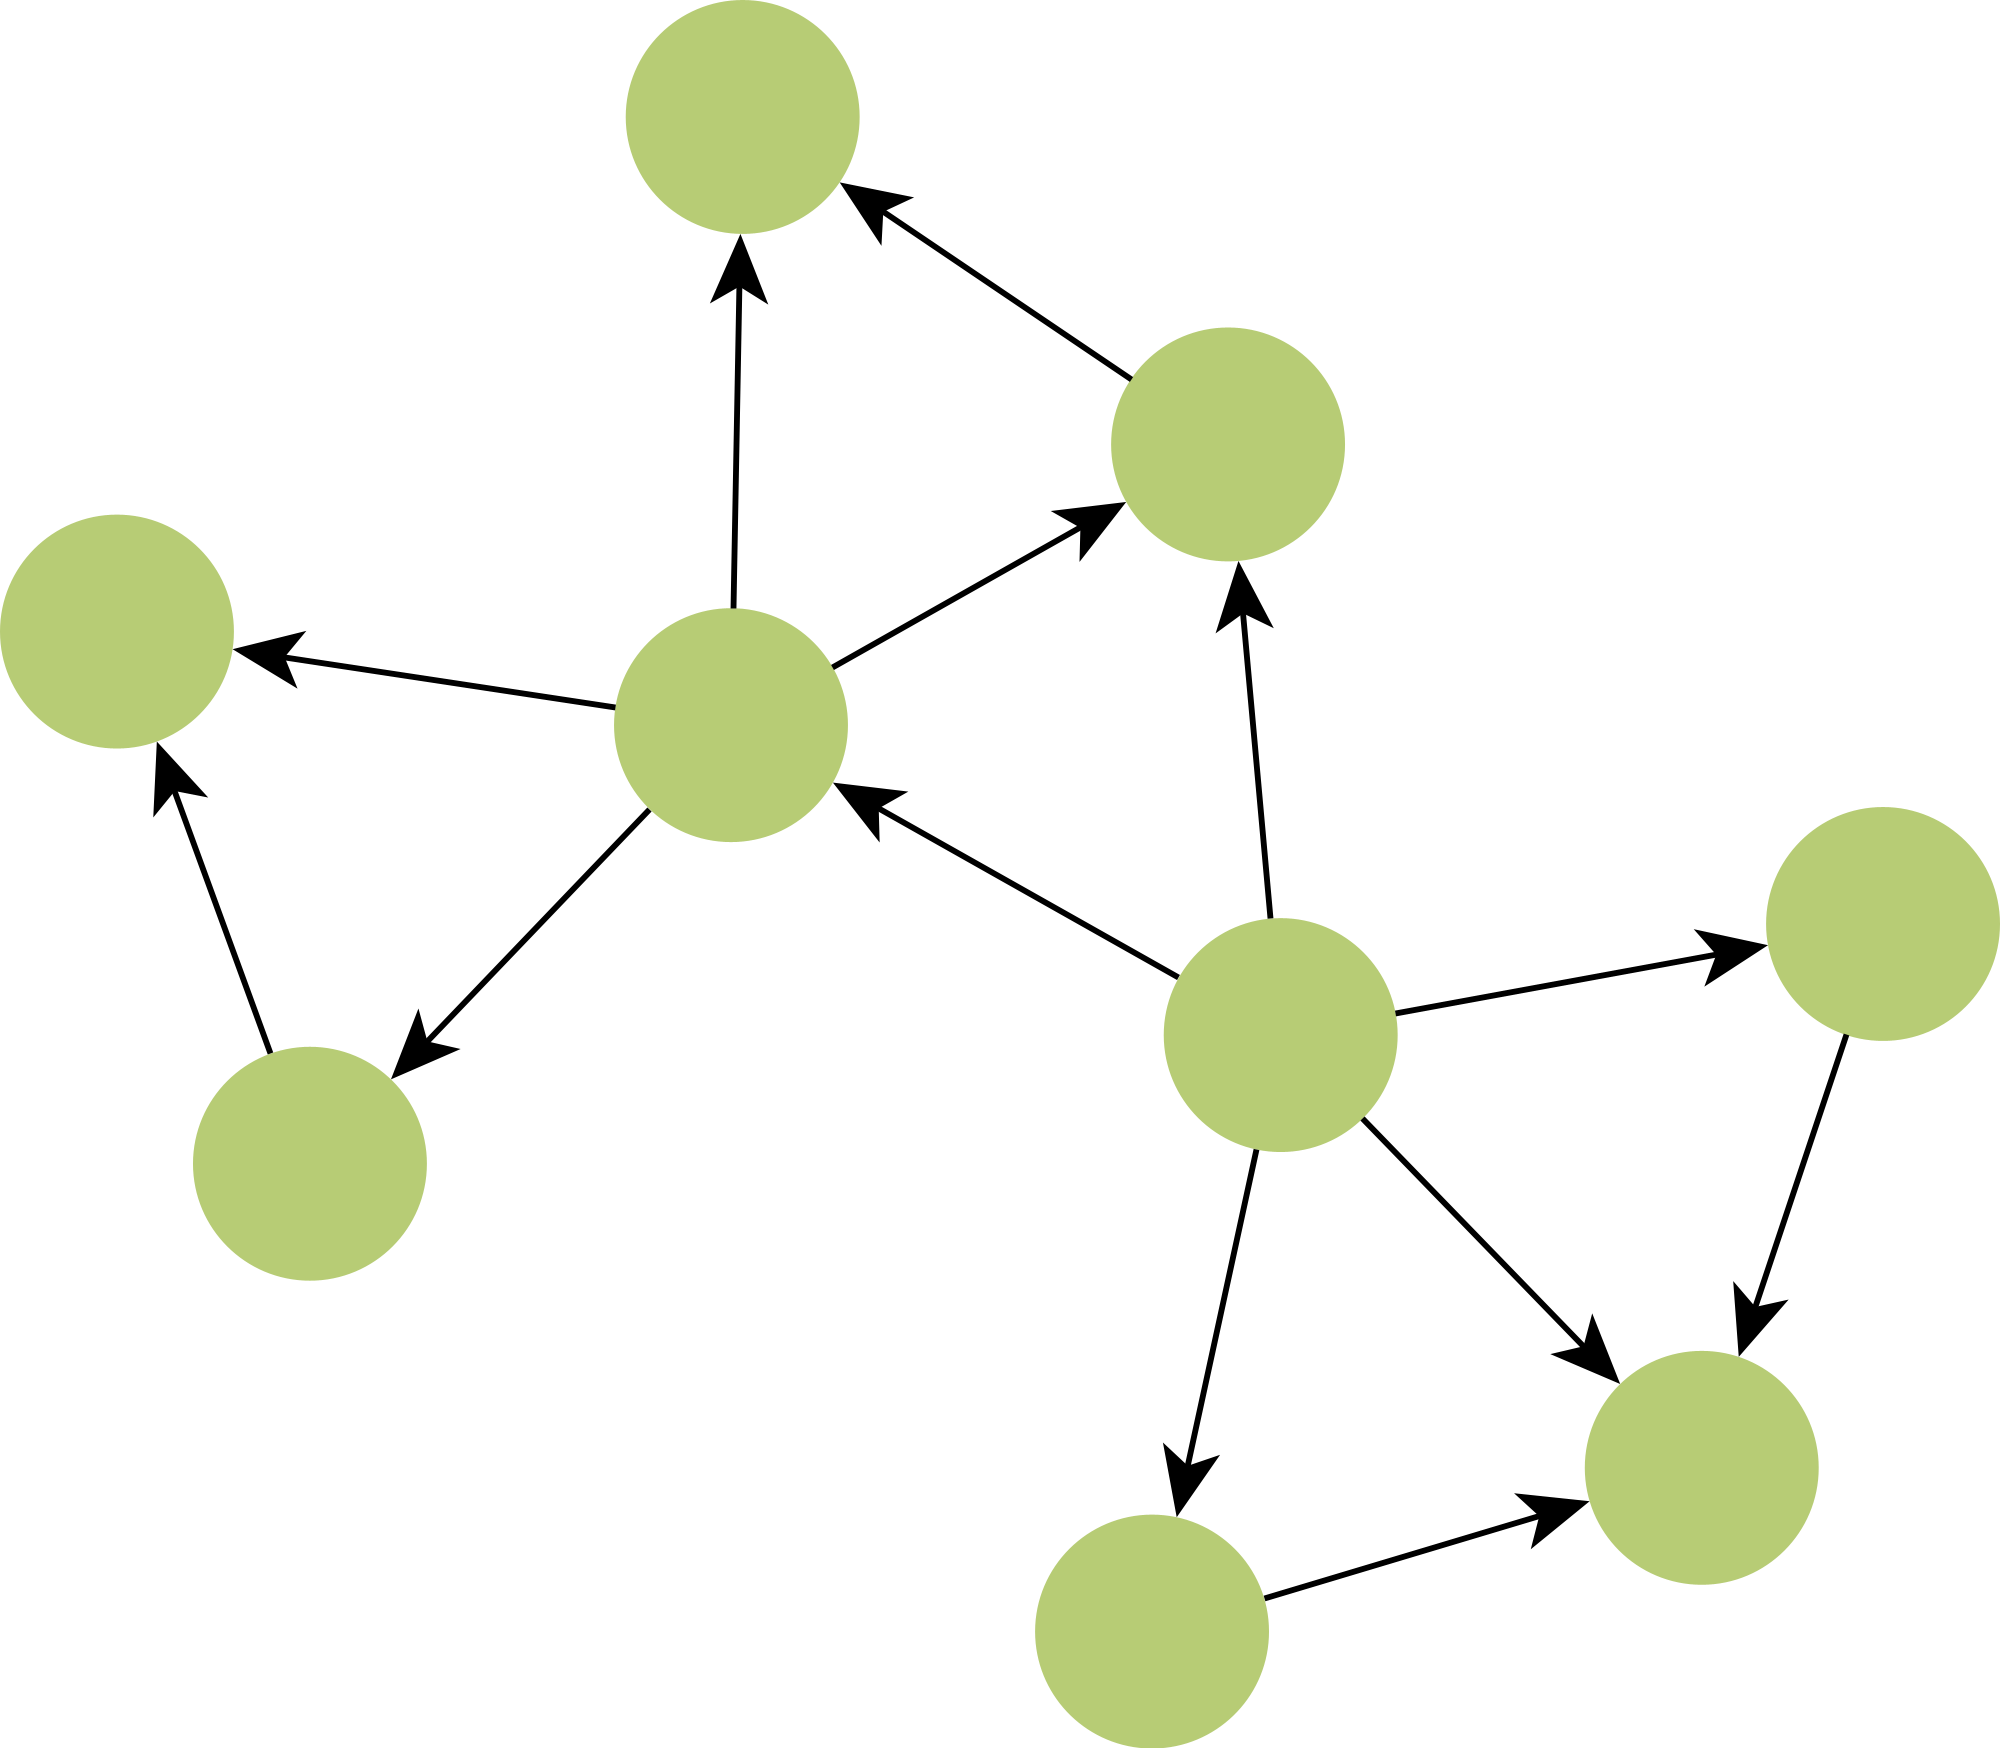
\includegraphics[width=7cm]{graphes2/img/graphe_sans_circuit.png}\\ \footnotesize graphe sans circuit\\
        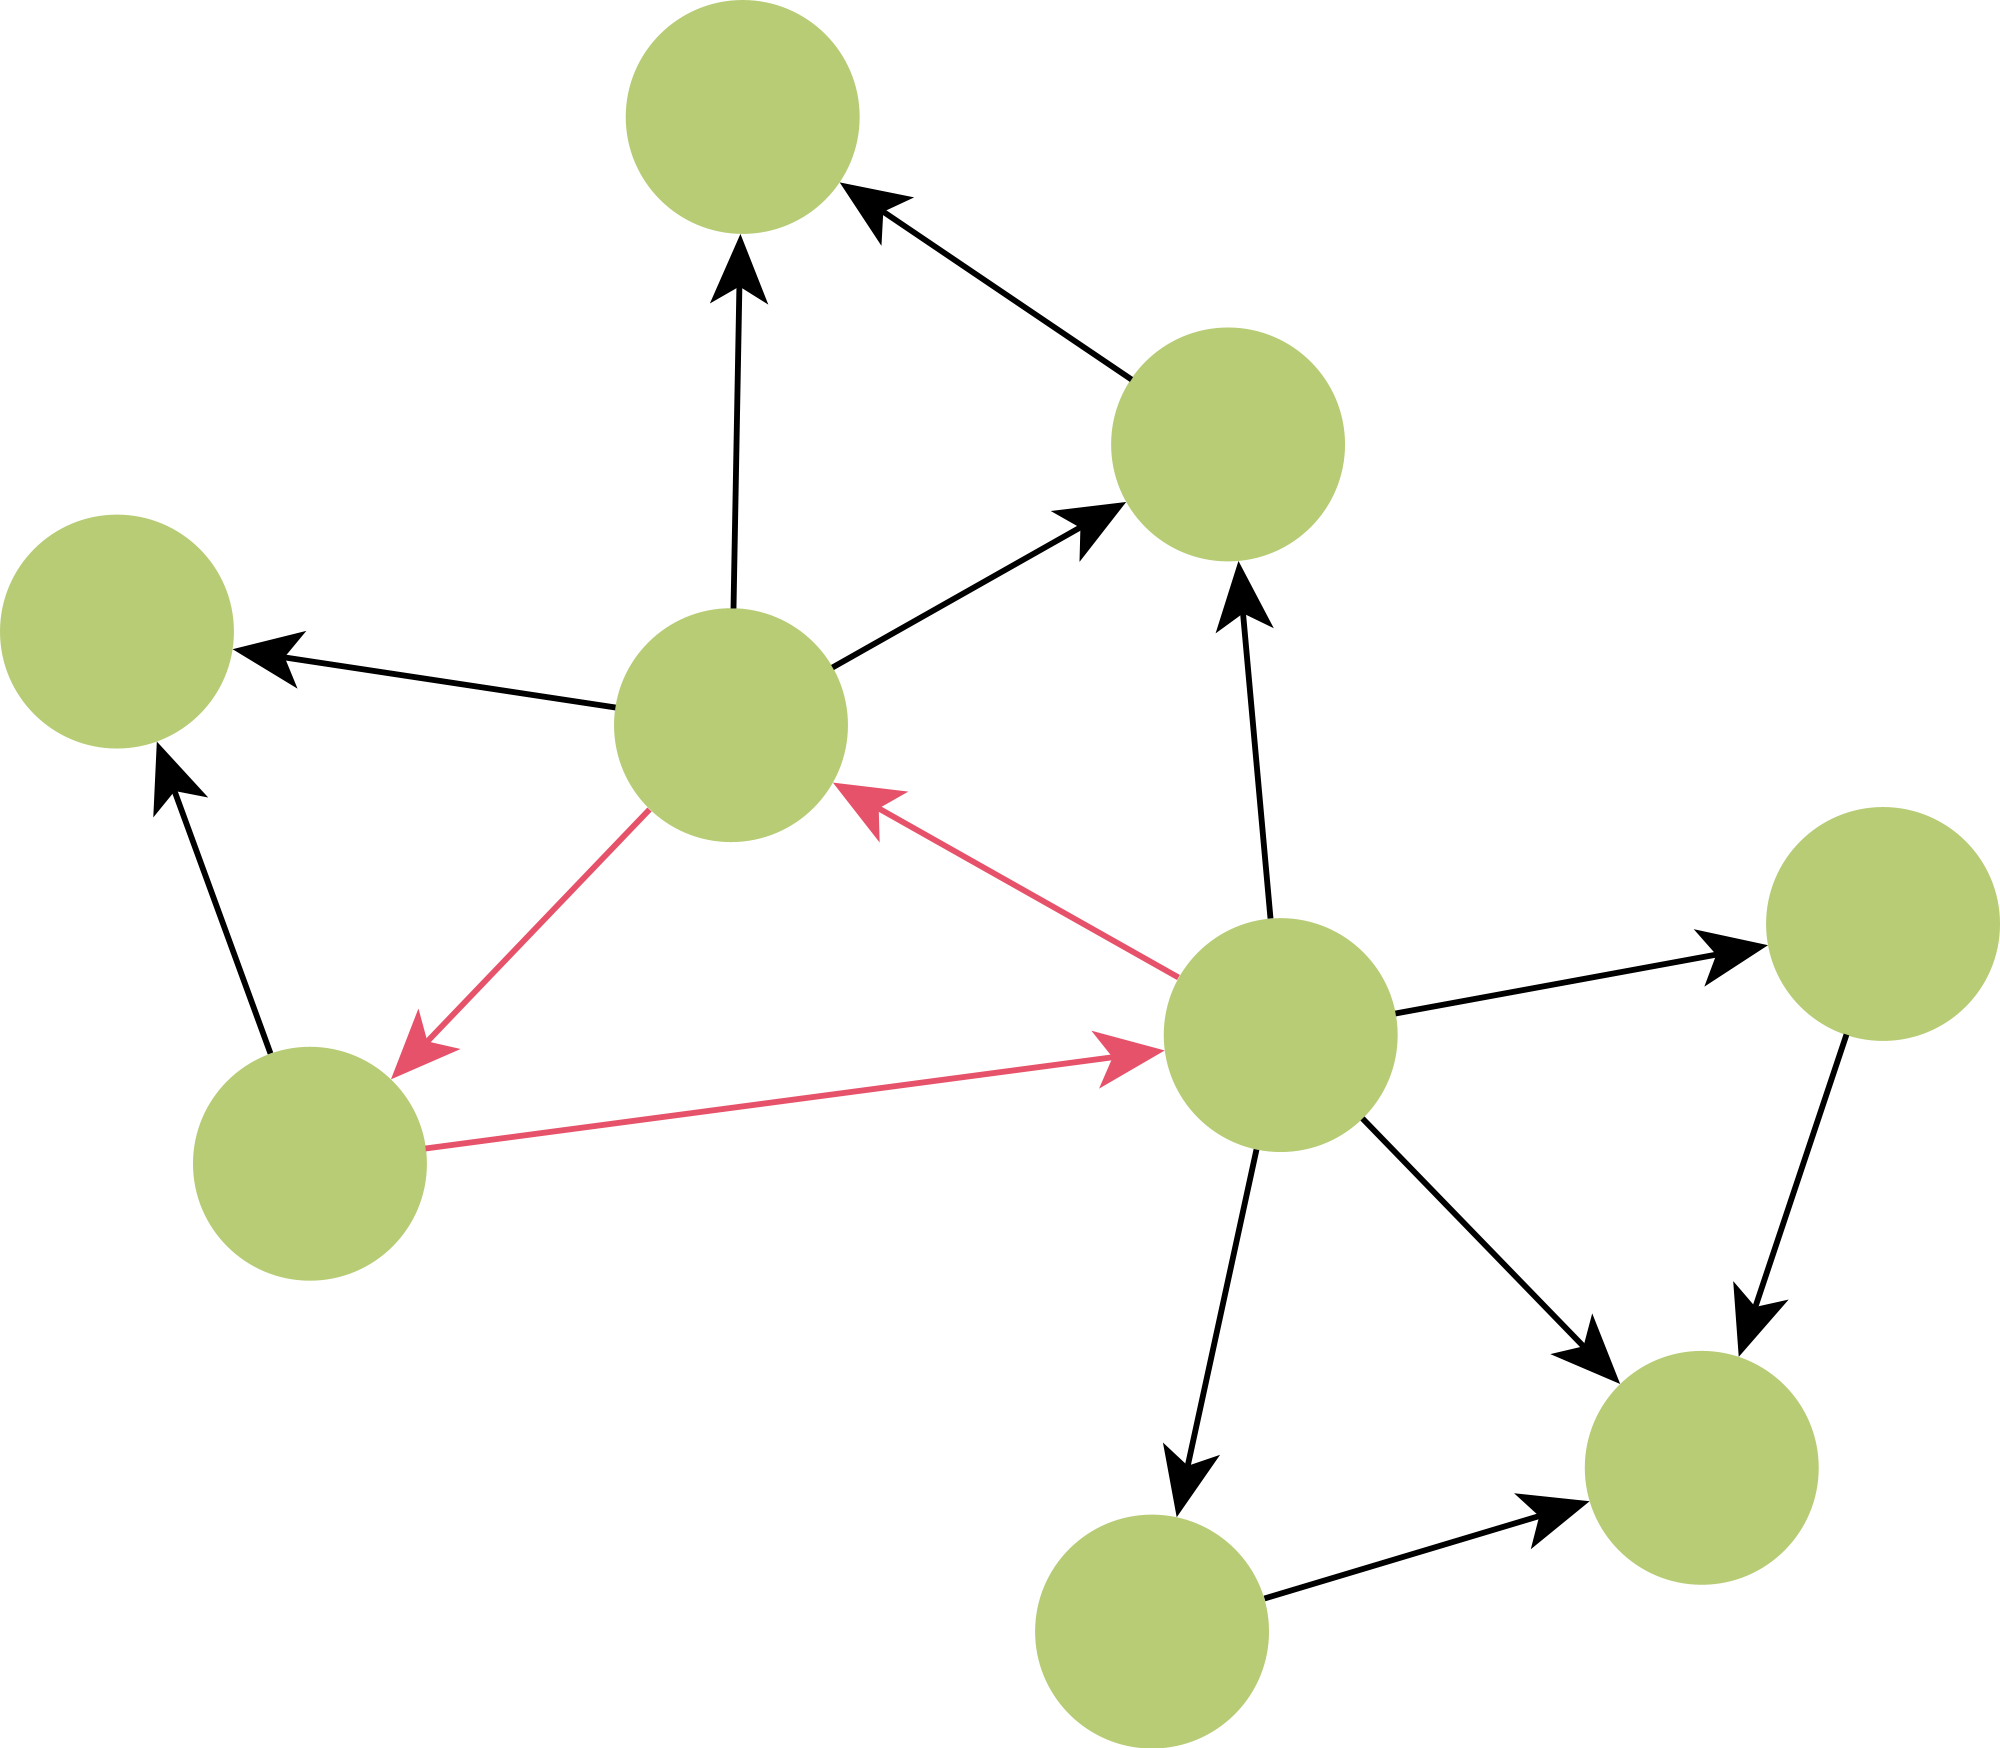
\includegraphics[width=7cm]{graphes2/img/graphe_avec_circuit.png}\\ \footnotesize graphe avec circuit
    \end{center}
\end{multicols}

Lorsqu'un graphe orienté est sans circuit il est possible de l'organiser de manière \textit{hiérarchisée}, comme ceci :
\begin{multicols}{2}
    \begin{center}
        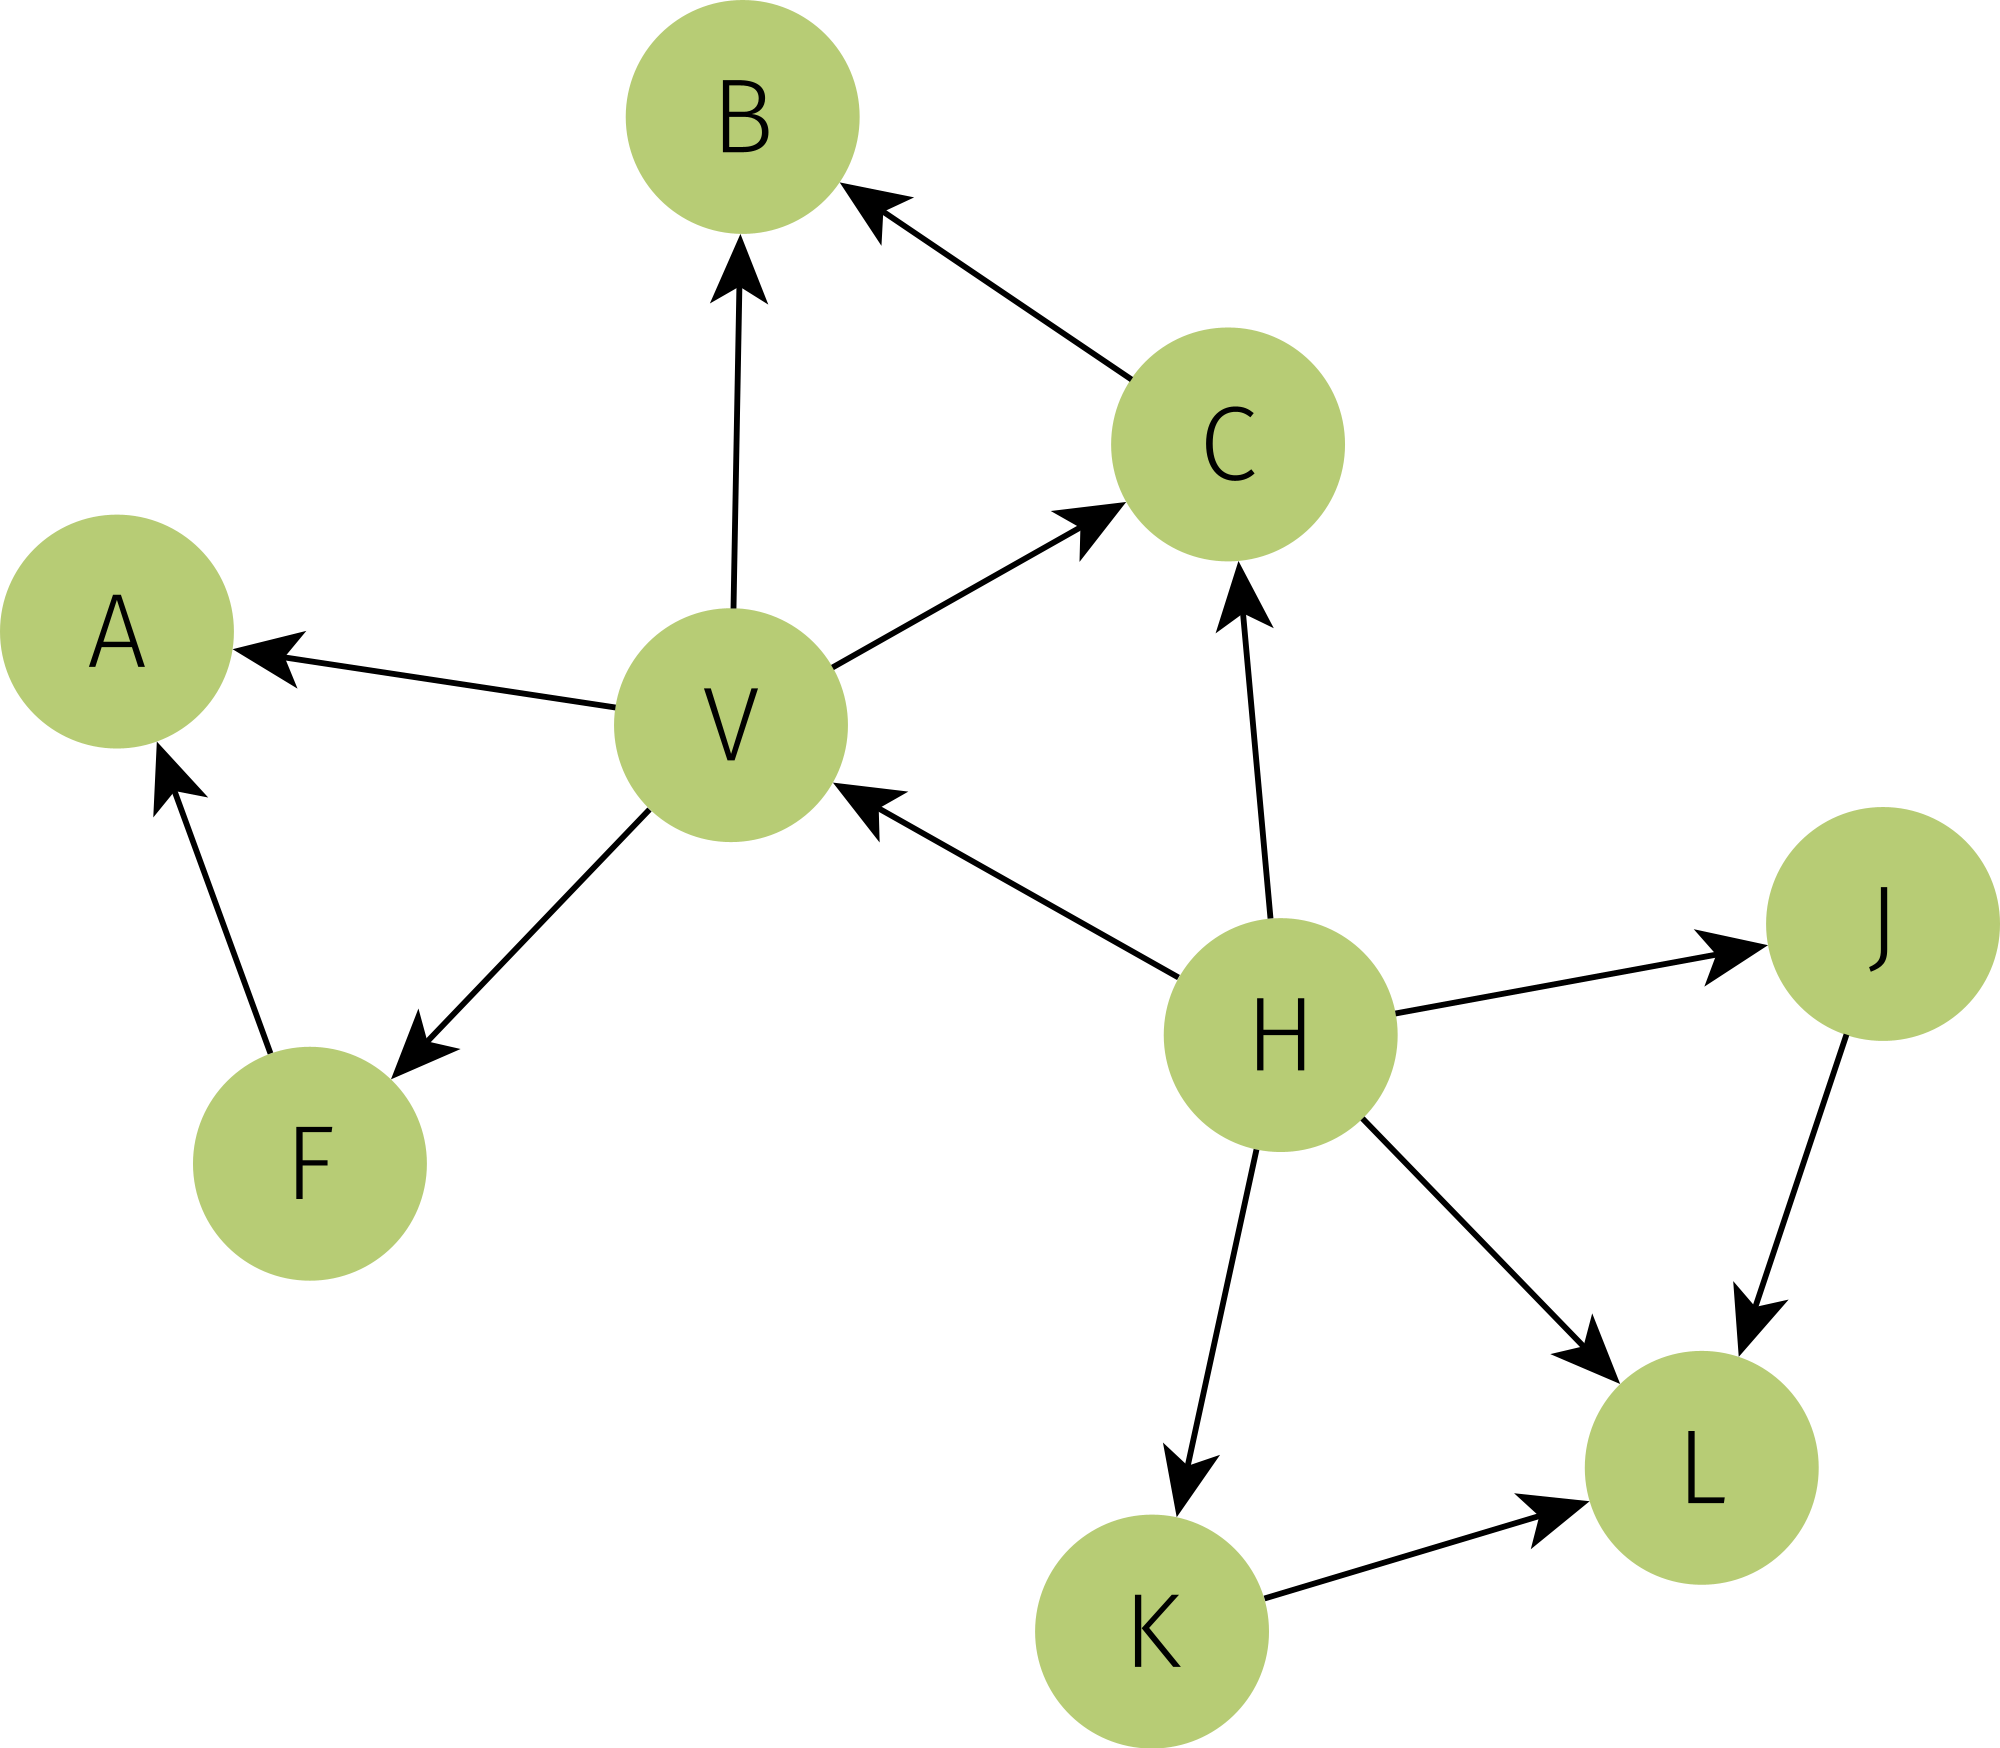
\includegraphics[width=7cm]{graphes2/img/graphe_sans_circuit_non_hierarchise.png}\\ \footnotesize graphe sans circuit\\
        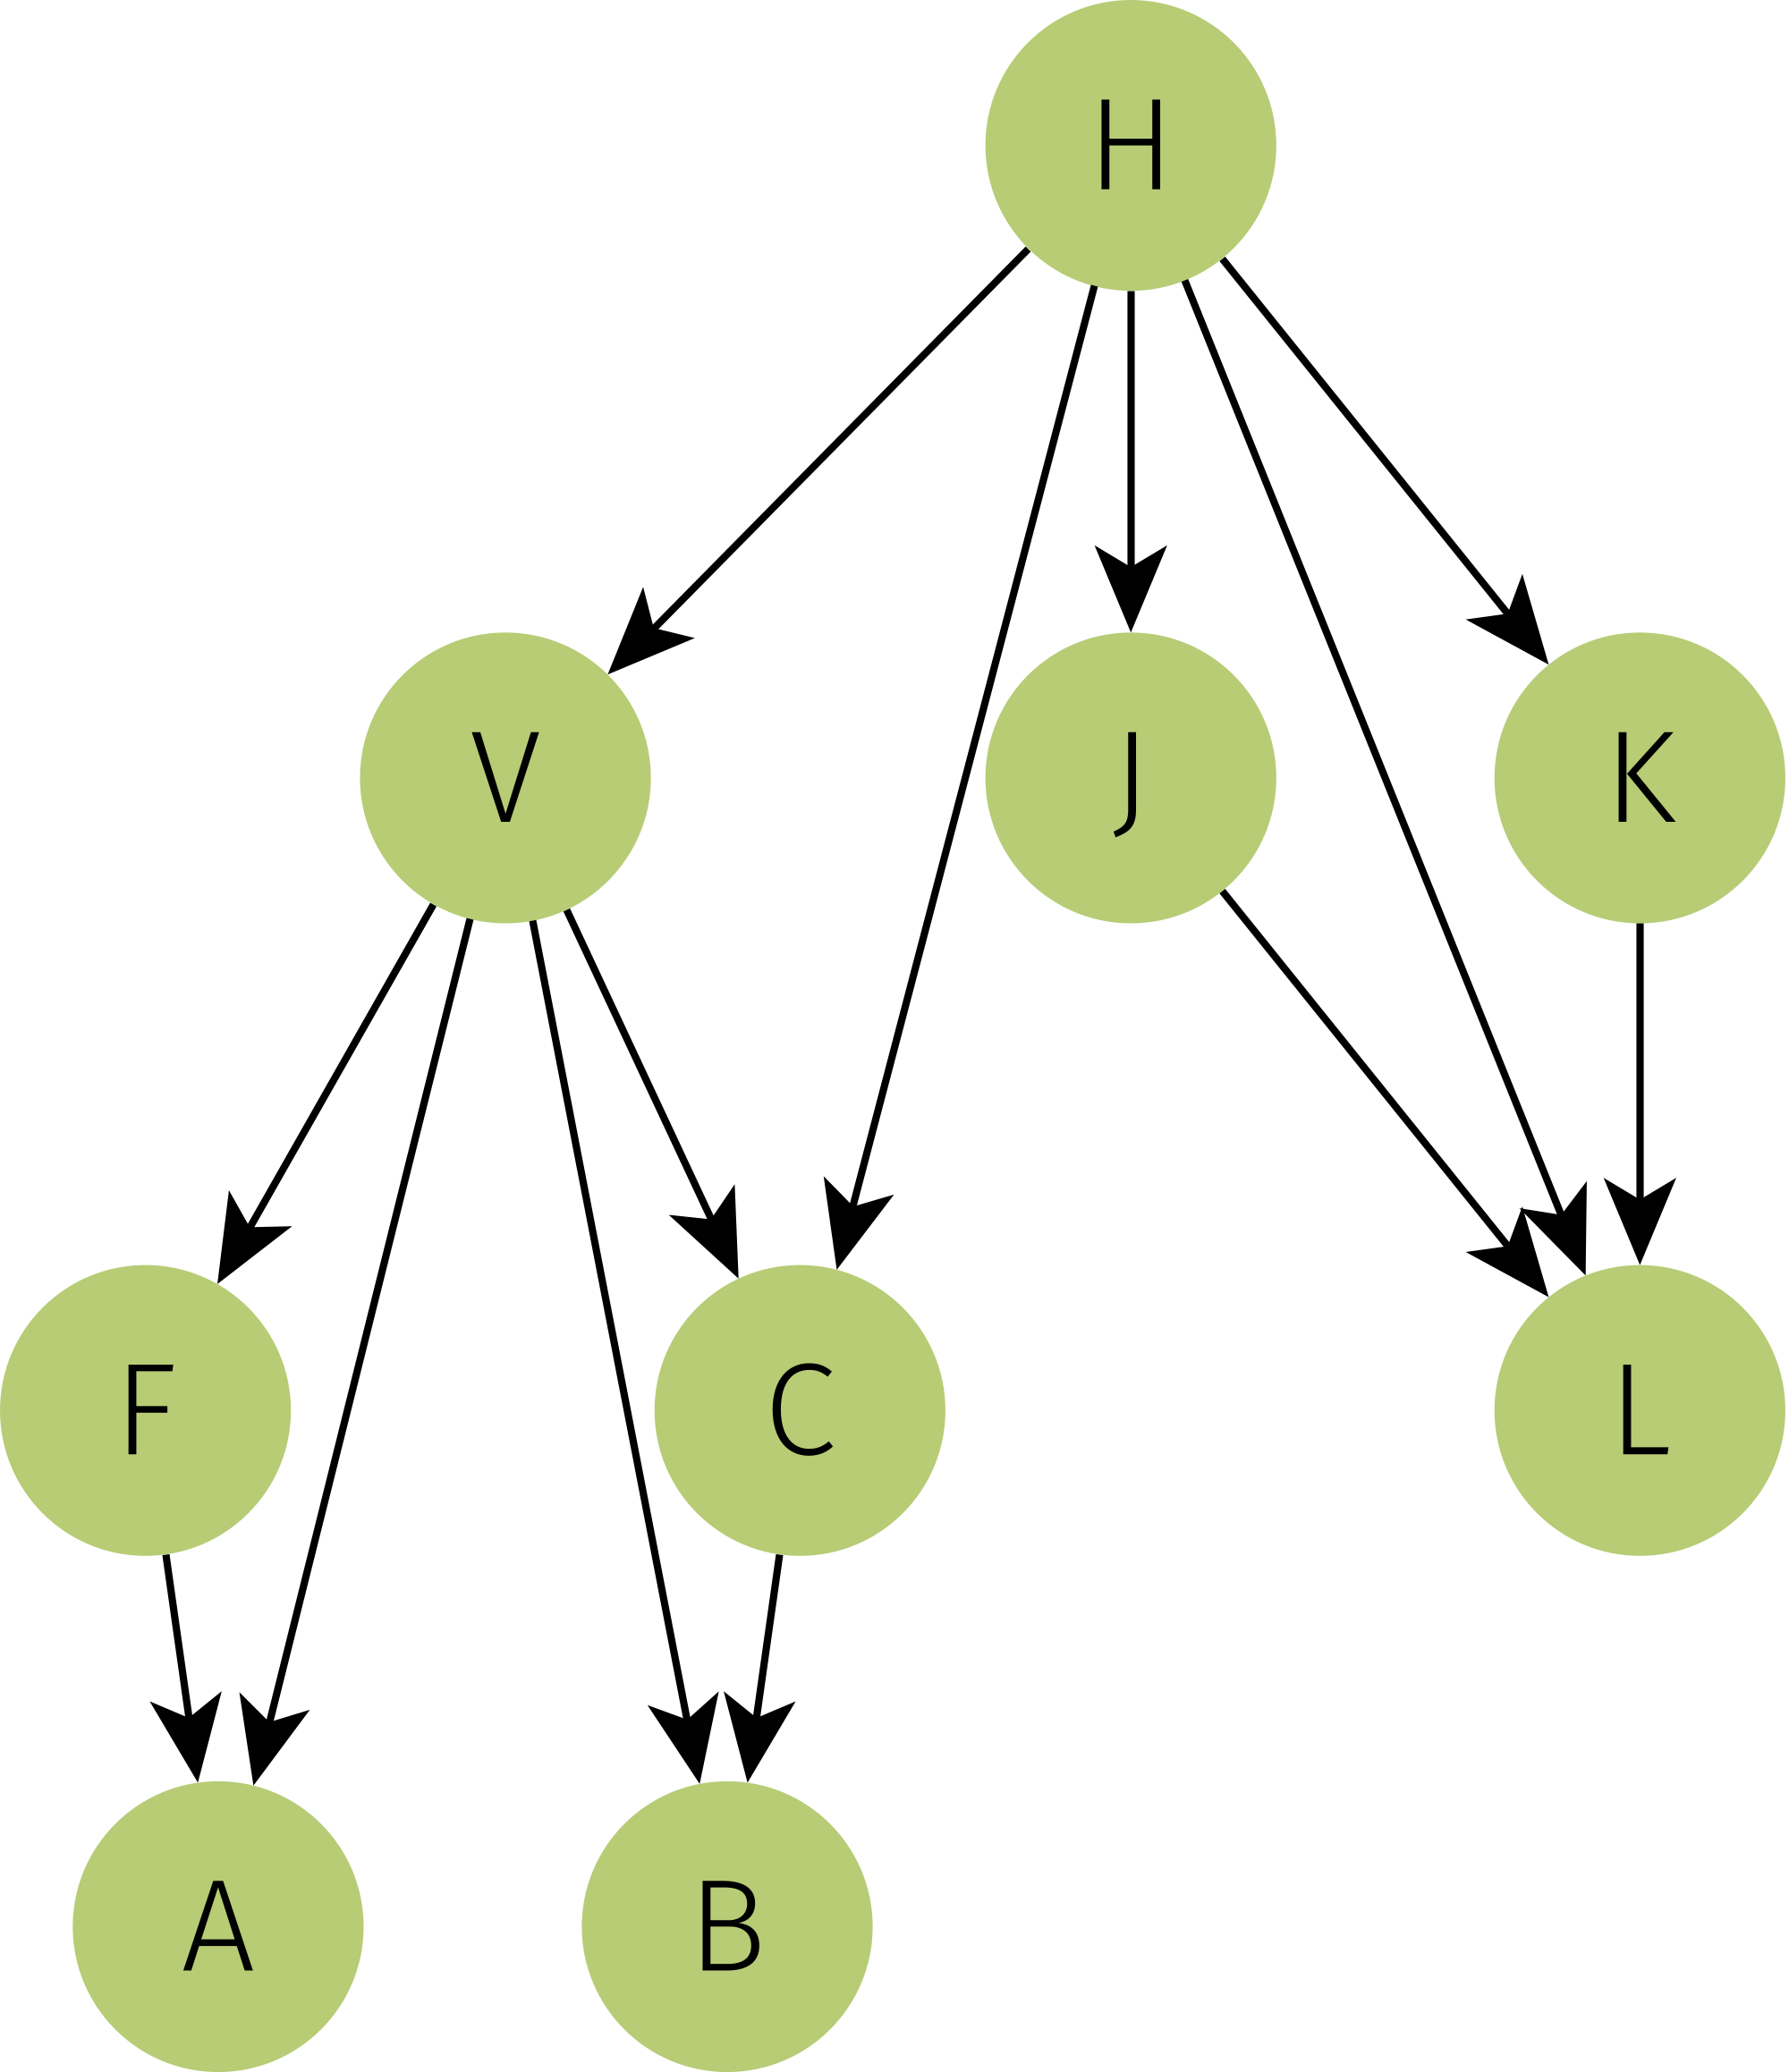
\includegraphics[width=5cm]{graphes2/img/graphe_sans_circuit_hierarchise.png}\\ \footnotesize le même graphe  hiérarchisé
    \end{center}
\end{multicols}

Comment faire ? À droite, on voit que les sommets sont disposés en couches horizontales : des \textit{niveaux}. Il faut donc définir ce qu'est le niveau d'un sommet.

\begin{propriete}[]
    Dans un graphe orienté sans circuit, il existe un sommet qui n'a pas de prédécesseur.
\end{propriete}
\begin{encadrecolore}{Preuve}{gray}
    Soit $n$ le nombre de sommets du graphe. On va raisonner par l'absurde : supposons que notre graphe soit sans circuit, mais qu'il n'existe aucun sommet sans prédécesseur. Alors tout sommet possède un prédécesseur.\\
    On en choisit un, on l'appelle  $S_0$ puis un de ses prédécesseurs qu' on appelle $S_1$
    \begin{itemize}
        \item 	si $S_1=S_0$ alors il y a une boucle (donc un circuit de longueur 1) sur $S_0$ et c'est contradictoire avec notre hypothèse.
        \item 	sinon on continue et on appelle $S_2$ un prédécesseur de $S_1$.
    \end{itemize}
    À chaque nouveau sommet choisi si c'est un sommet qui figure déjà dans la liste des sommets choisis, cela nous permet d'exhiber un circuit et c'est contradictoire. Or comme il n'y a que $n$ sommets, au bout de $n$ étapes (au maximum), on sera obligés de choisir un sommet déjà choisi.
\end{encadrecolore}


\begin{definition}[ : niveau d'un sommet dans un graphe orienté sans circuit]
    Soit un sommet d'un graphe orienté sans circuit
    \begin{itemize}
        \item 	s'il n'a pas de prédécesseur, son niveau est 0;
        \item 	sinon, on considère tous ses prédécesseurs, on choisit celui qui a le niveau le plus élevé et on ajoute 1 : on obtient le niveau du sommet.
    \end{itemize}
\end{definition}

Pour déterminer les niveaux des sommets on peut aussi appliquer l'algorithme suivant :
\begin{verbatim}
Variables
    L : liste des sommets
    n : entier 
Début
    n <-- 0
    tant que L est non vide
        sélectionner tous les sommets qui n'ont aucun prédécesseur dans L
        ils ont le niveau n
        enlever ces sommets de L
	    n <-- n + 1
Fin
\end{verbatim}


\begin{exemple}[]
    On considère le graphe suivant :
    \begin{center}
        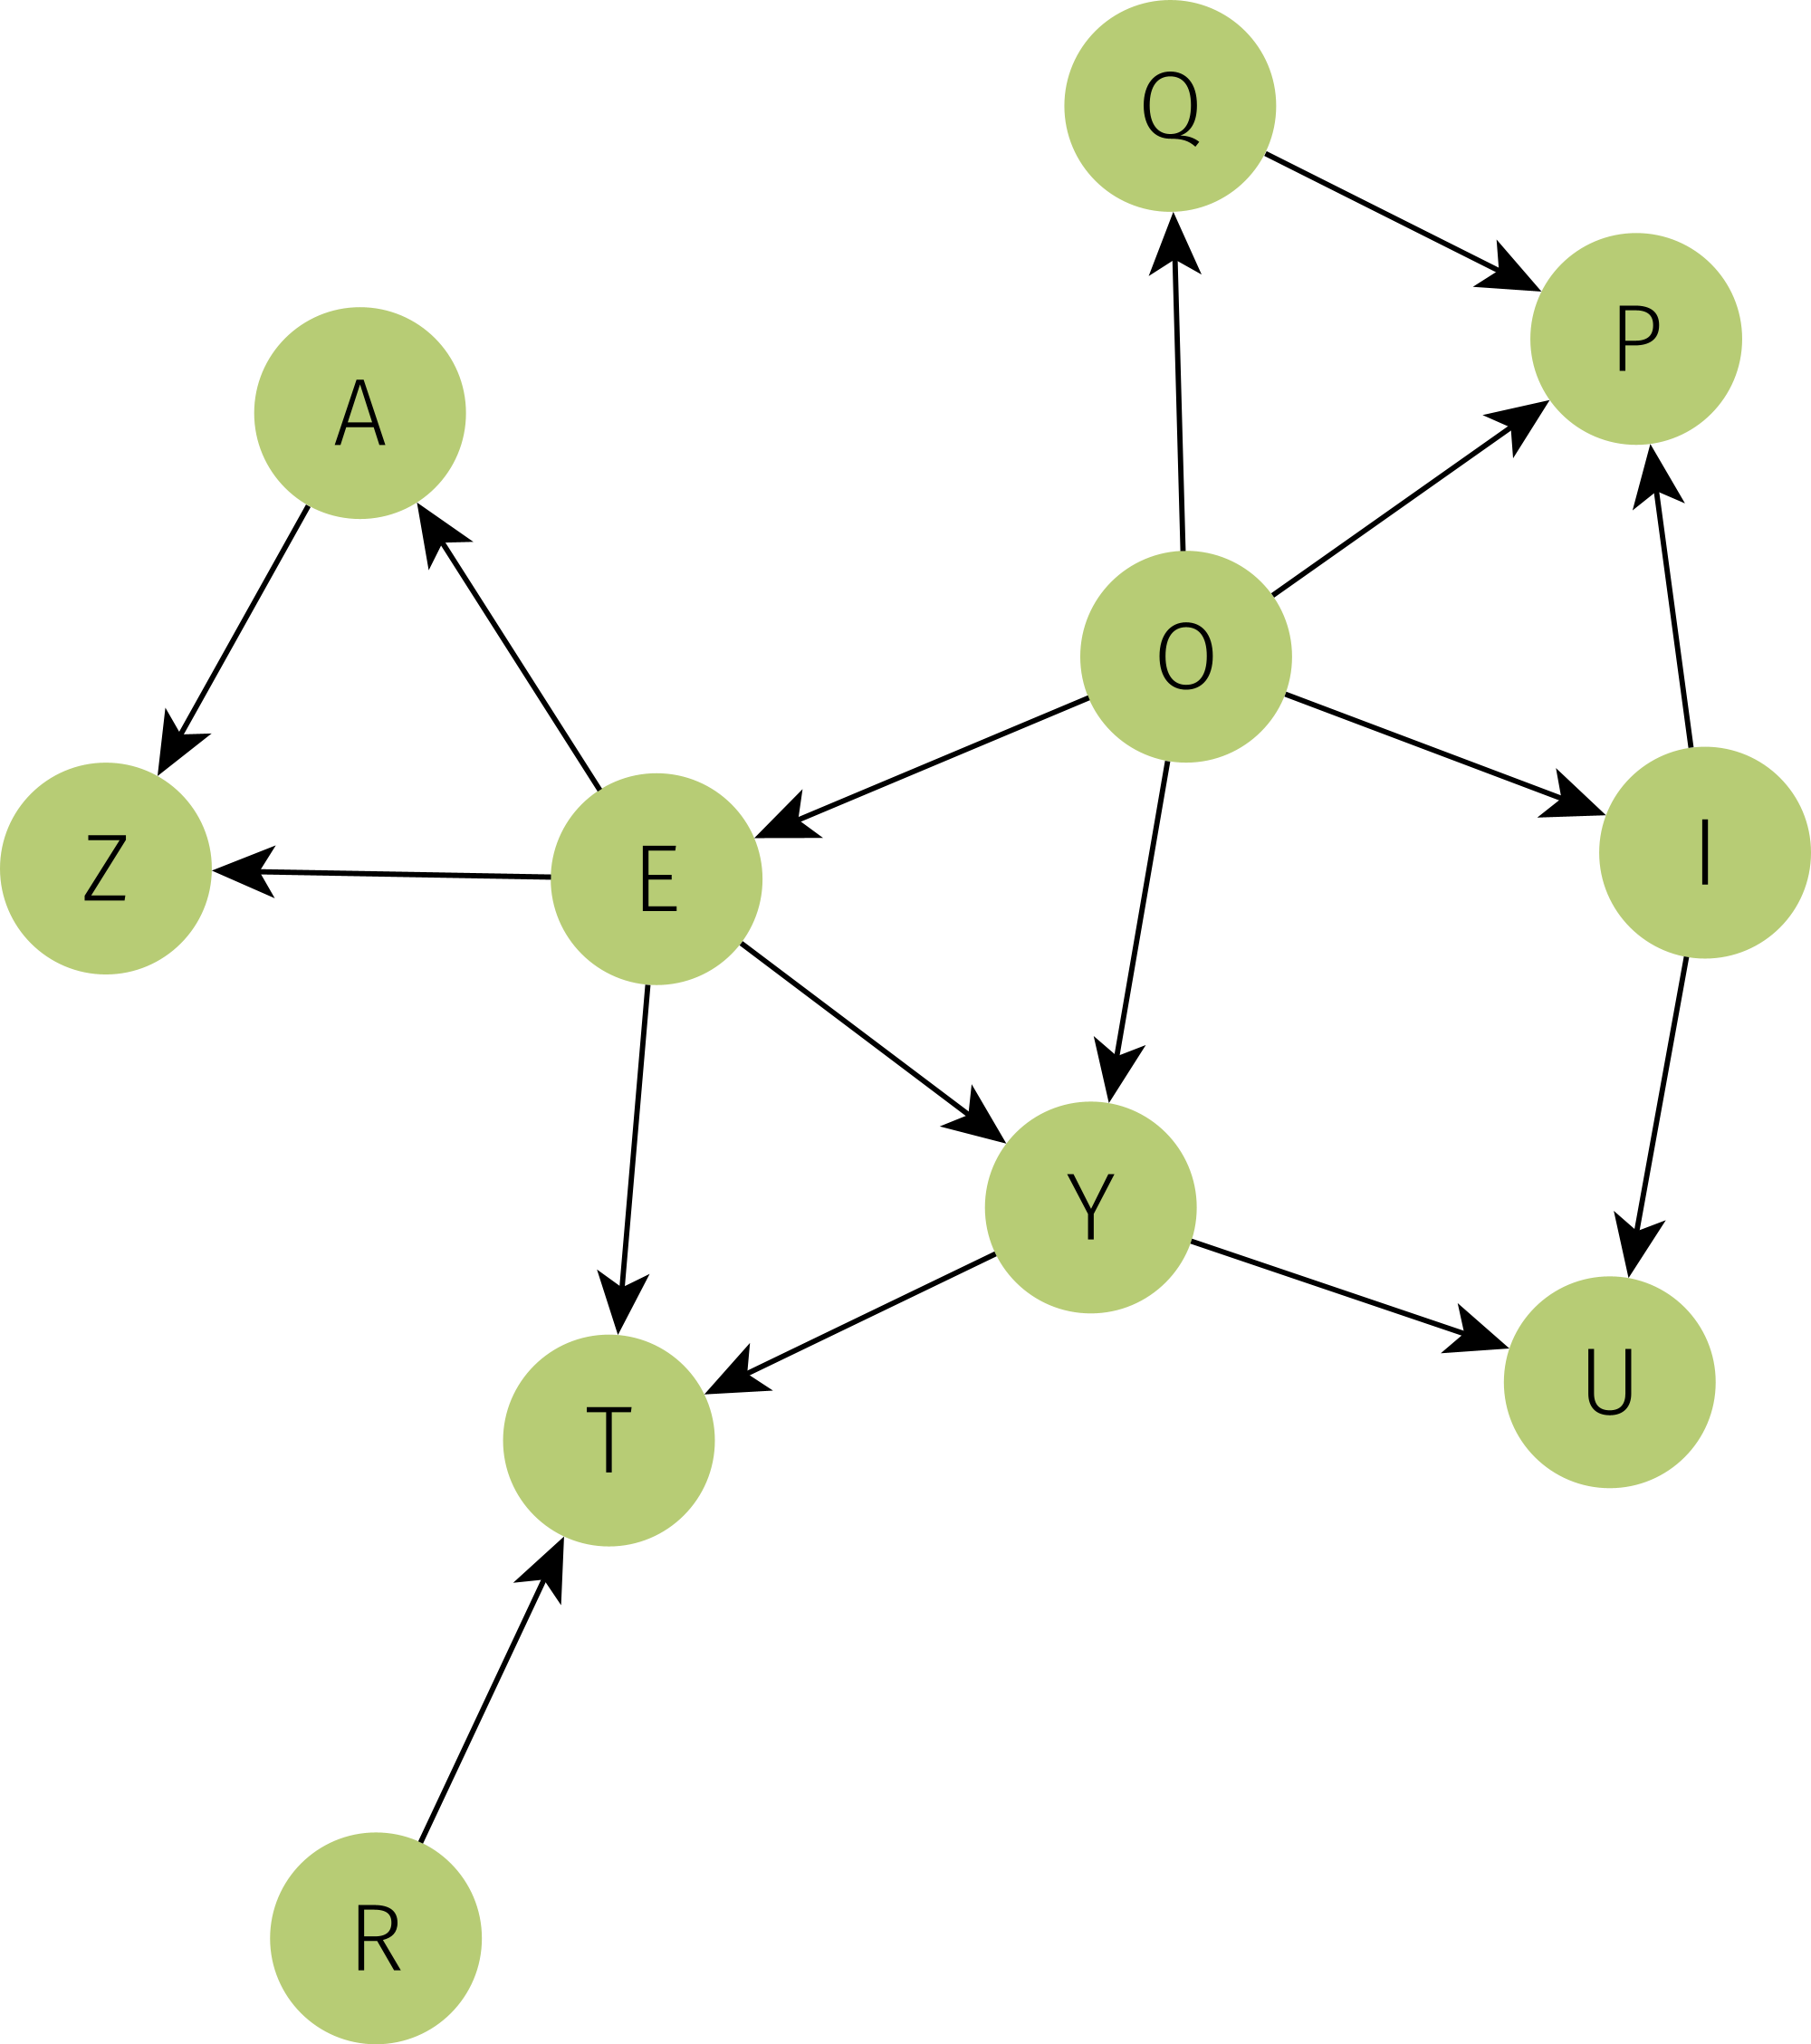
\includegraphics[width=7cm]{graphes2/img/nivellement_exemple.png}
    \end{center}
    On commence par construire le tableau des prédécesseurs :\\

    \def\ltb{.6cm}
    \tabstyled
    \begin{tabular}{|l|>{\centering\arraybackslash}m{\ltb}|>{\centering\arraybackslash}m{\ltb}|>{\centering\arraybackslash}m{\ltb}|>{\centering\arraybackslash}m{\ltb}|>{\centering\arraybackslash}m{\ltb}|>{\centering\arraybackslash}m{\ltb}|>{\centering\arraybackslash}m{\ltb}|>{\centering\arraybackslash}m{\ltb}|>{\centering\arraybackslash}m{\ltb}|>{\centering\arraybackslash}m{\ltb}|>{\centering\arraybackslash}m{\ltb}|}
        \hline
        \ccell sommet        & A & Z   & E & R   & T     & Y   & U   & I & O   & P     & Q \\
        \hline
        \ccell prédécesseurs & E & A,E & O & --- & R,E,Y & E,O & Y,I & O & --- & I,O,Q & O \\
        \hline
    \end{tabular}\\

    R et O ont le niveau 0. On les retire du tableau :\\

    \tabstyled
    \begin{tabular}{|l|>{\centering\arraybackslash}m{\ltb}|>{\centering\arraybackslash}m{\ltb}|>{\centering\arraybackslash}m{\ltb}|>{\centering\arraybackslash}m{\ltb}|>{\centering\arraybackslash}m{\ltb}|>{\centering\arraybackslash}m{\ltb}|>{\centering\arraybackslash}m{\ltb}|>{\centering\arraybackslash}m{\ltb}|>{\centering\arraybackslash}m{\ltb}|}
        \hline
        \ccell sommet        & A & Z   & E   & T   & Y & U   & I   & P   & Q   \\
        \hline
        \ccell prédécesseurs & E & A,E & --- & E,Y & E & Y,I & --- & I,Q & --- \\
        \hline
    \end{tabular}\\

    E, I et Q ont le niveau 1, on les retire :\\
    \tabstyled
    \begin{tabular}{|l|>{\centering\arraybackslash}m{\ltb}|>{\centering\arraybackslash}m{\ltb}|>{\centering\arraybackslash}m{\ltb}|>{\centering\arraybackslash}m{\ltb}|>{\centering\arraybackslash}m{\ltb}|>{\centering\arraybackslash}m{\ltb}|}
        \hline
        \ccell sommet        & A   & Z & T & Y   & U & P   \\
        \hline
        \ccell prédécesseurs & --- & A & Y & --- & Y & --- \\
        \hline
    \end{tabular}\\

    A, Y et P ont le niveau 2 et on voit que Z, T et U ont le niveau 3.\\

    \tabstyled
    \def\ltb{.75cm}
    \begin{tabular}{|l|>{\centering\arraybackslash}m{\ltb}|>{\centering\arraybackslash}m{\ltb}|>{\centering\arraybackslash}m{\ltb}|>{\centering\arraybackslash}m{\ltb}|>{\centering\arraybackslash}m{\ltb}|>{\centering\arraybackslash}m{\ltb}|>{\centering\arraybackslash}m{\ltb}|>{\centering\arraybackslash}m{\ltb}|>{\centering\arraybackslash}m{\ltb}|>{\centering\arraybackslash}m{\ltb}|>{\centering\arraybackslash}m{\ltb}|}
        \hline
        \ccell sommet & R & O & E & I & Q & A & Y & P & Z & T & U \\
        \hline
        \ccell niveau & 0 & 0 & 1 & 1 & 1 & 2 & 2 & 2 & 3 & 3 & 3 \\
        \hline
    \end{tabular}\\

    On peut maintenant redessiner le graphe de manière hiérarchisée de haut en bas ou de droite à gauche, en alignant les sommets par niveaux :

    \begin{center}
        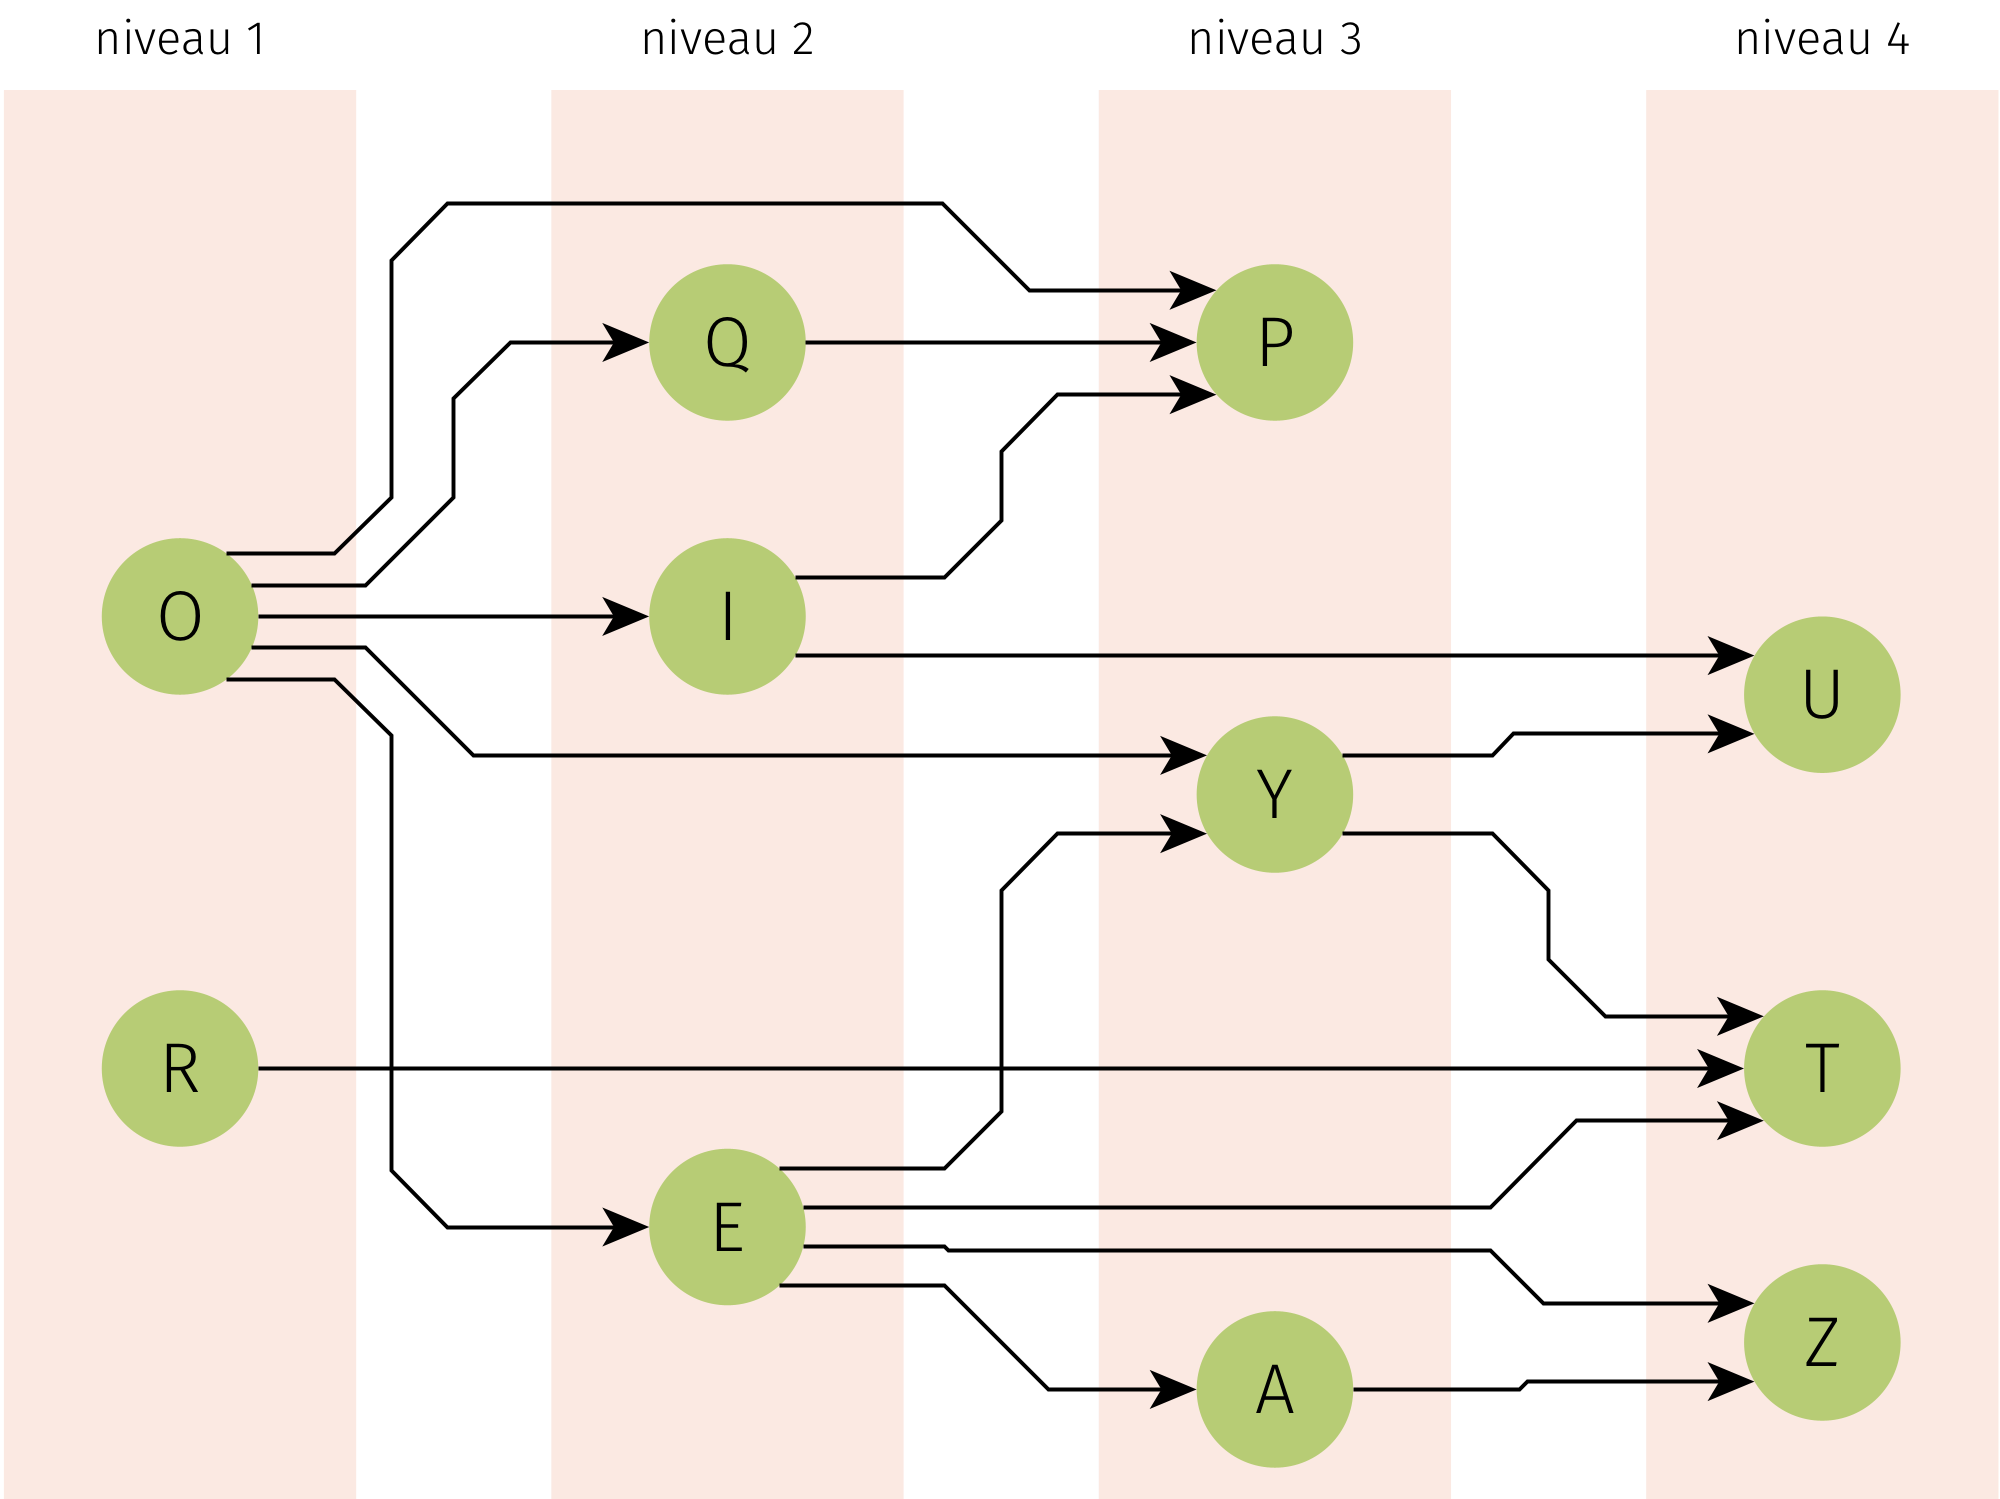
\includegraphics[width=10cm]{graphes2/img/nivellement_exemple_fait.png}\\ {\footnotesize graphe représenté de manière nivelée}

    \end{center}
\end{exemple}

En appliquant cette méthode on peut parfois prouver qu'un graphe donné est une \textit{arborescence}.

\begin{definition}[ : arborescence]
    Une \textit{arborescence} est un graphe oriente qui possède \textit{un unique sommet de niveau 0}, qu'on appelle la \textit{racine} et à partir de laquelle on peut atteindre \textit{tout autre sommet par un unique chemin}.
    \begin{multicols}{2}
        \begin{center}
            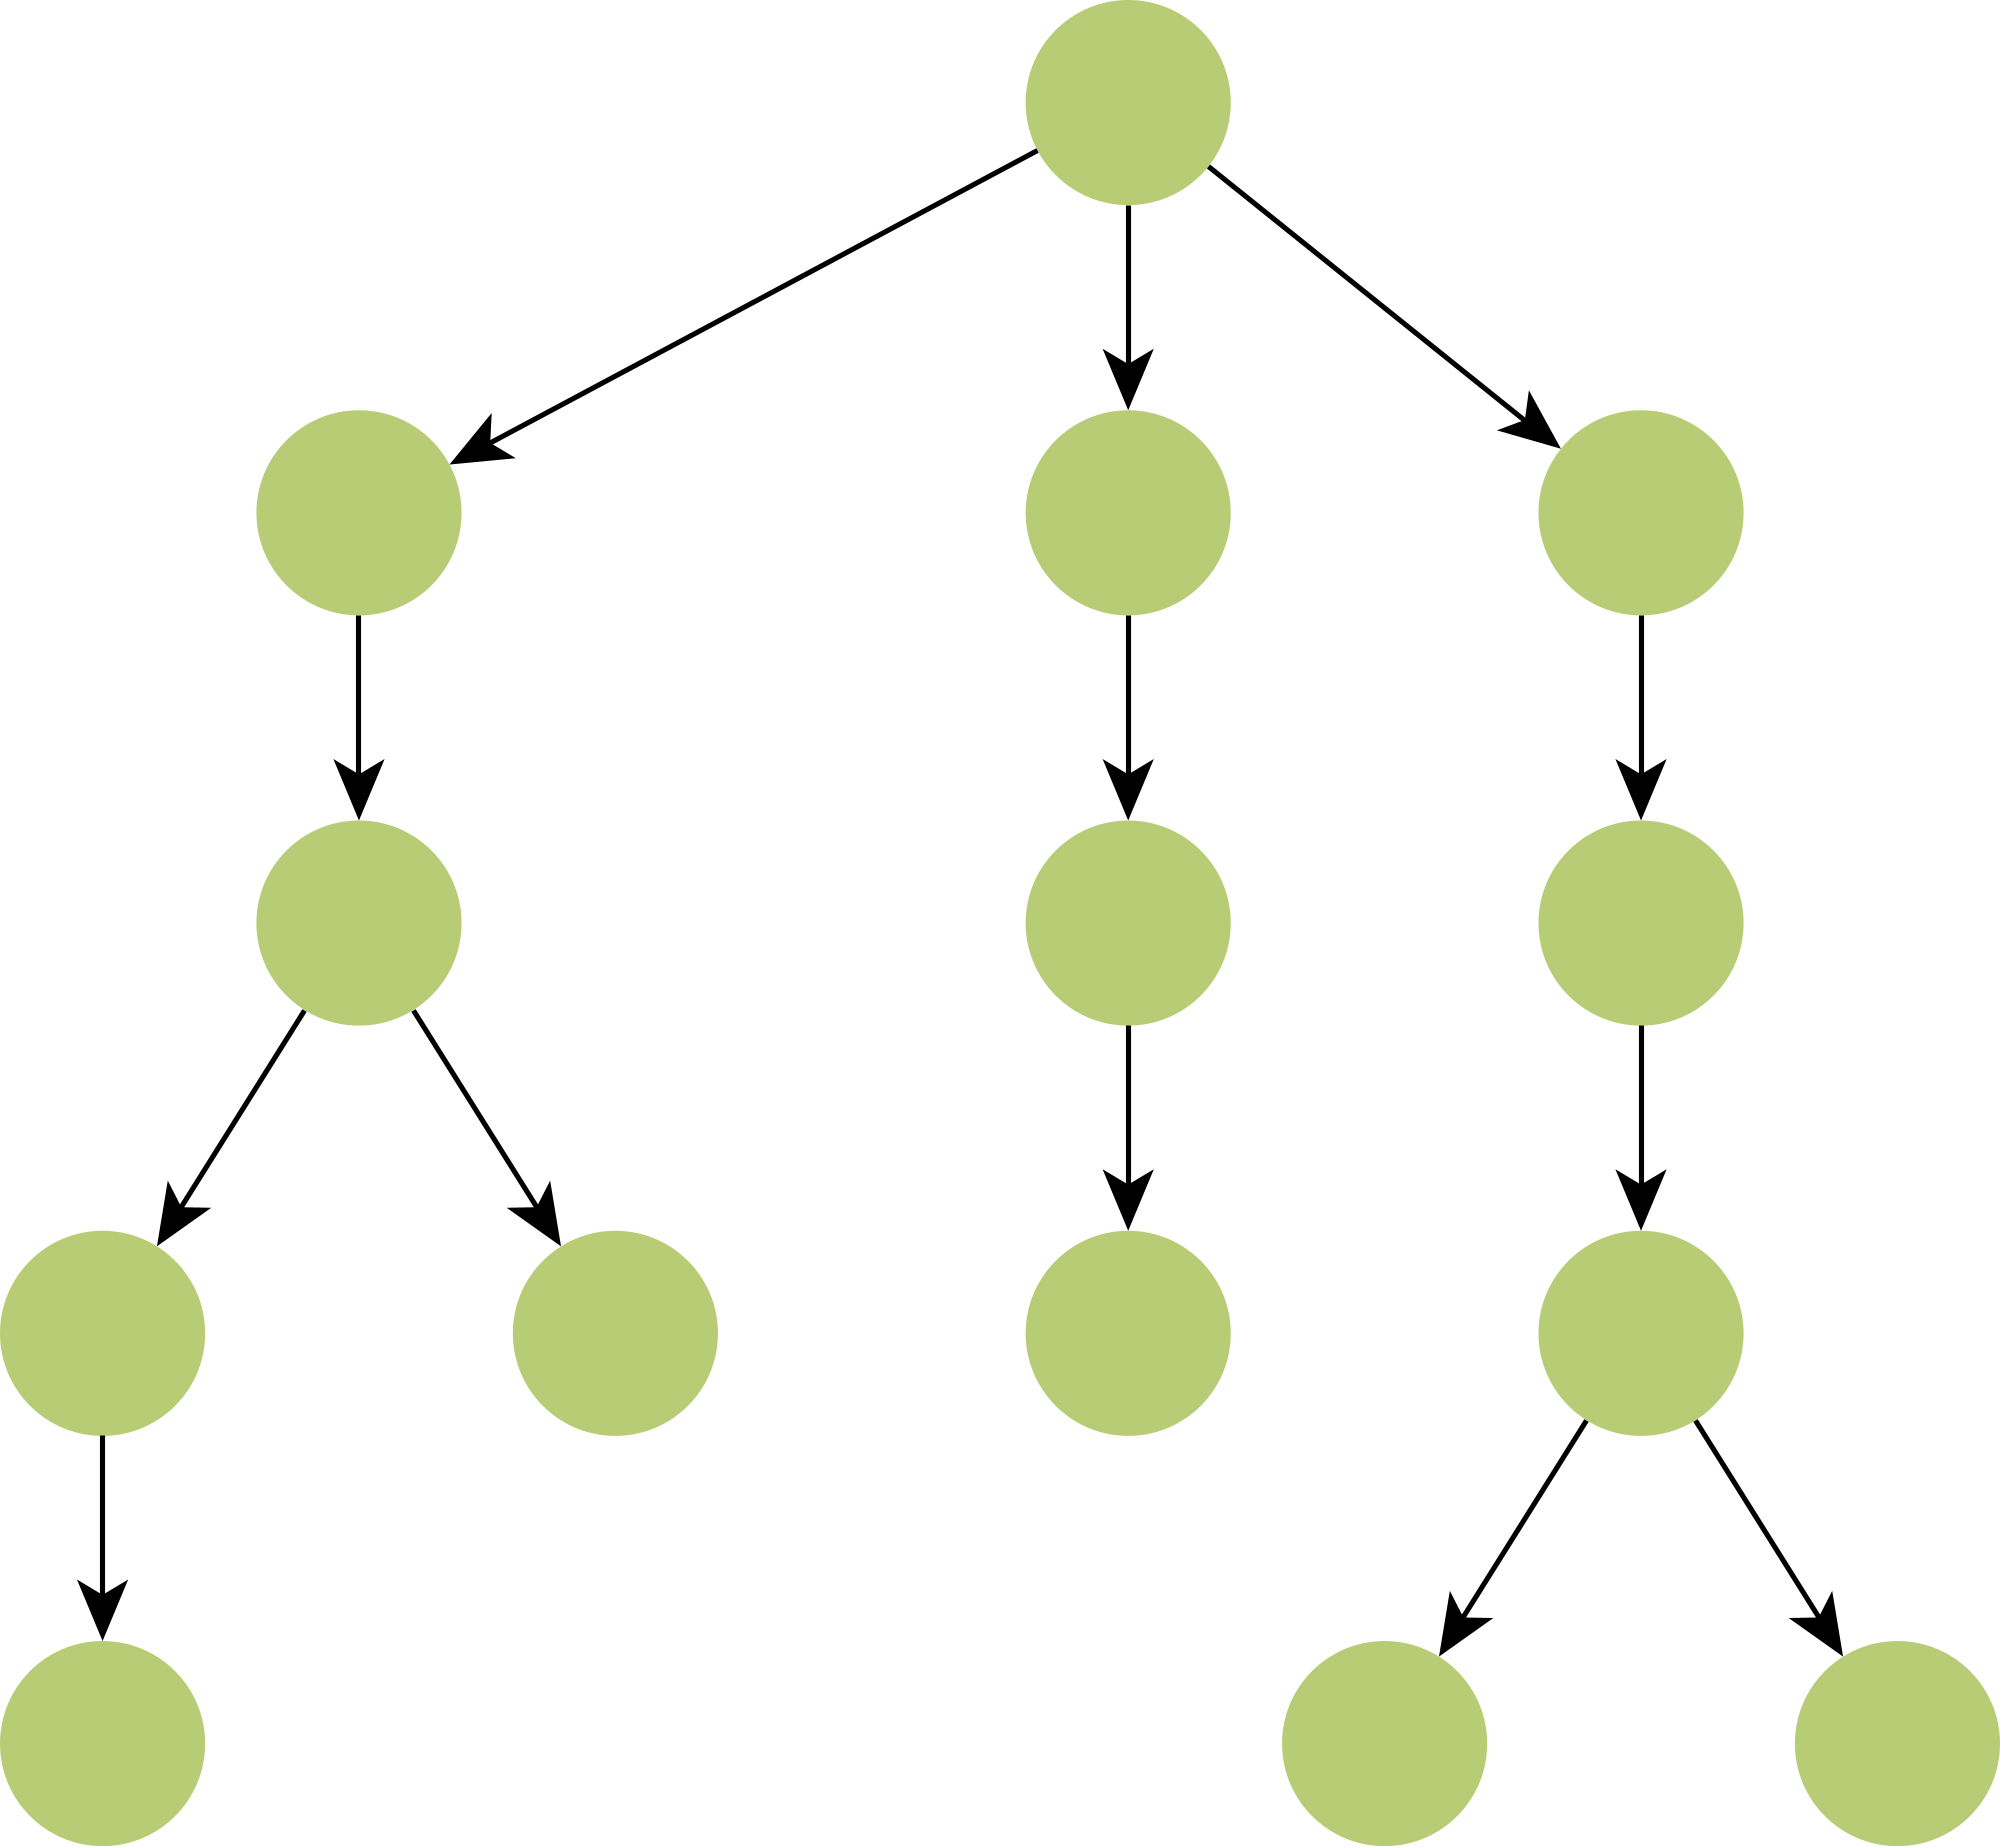
\includegraphics[width=7cm]{graphes2/img/ex_arborescence.png}\\ \footnotesize graphe qui est une arborescence\\
            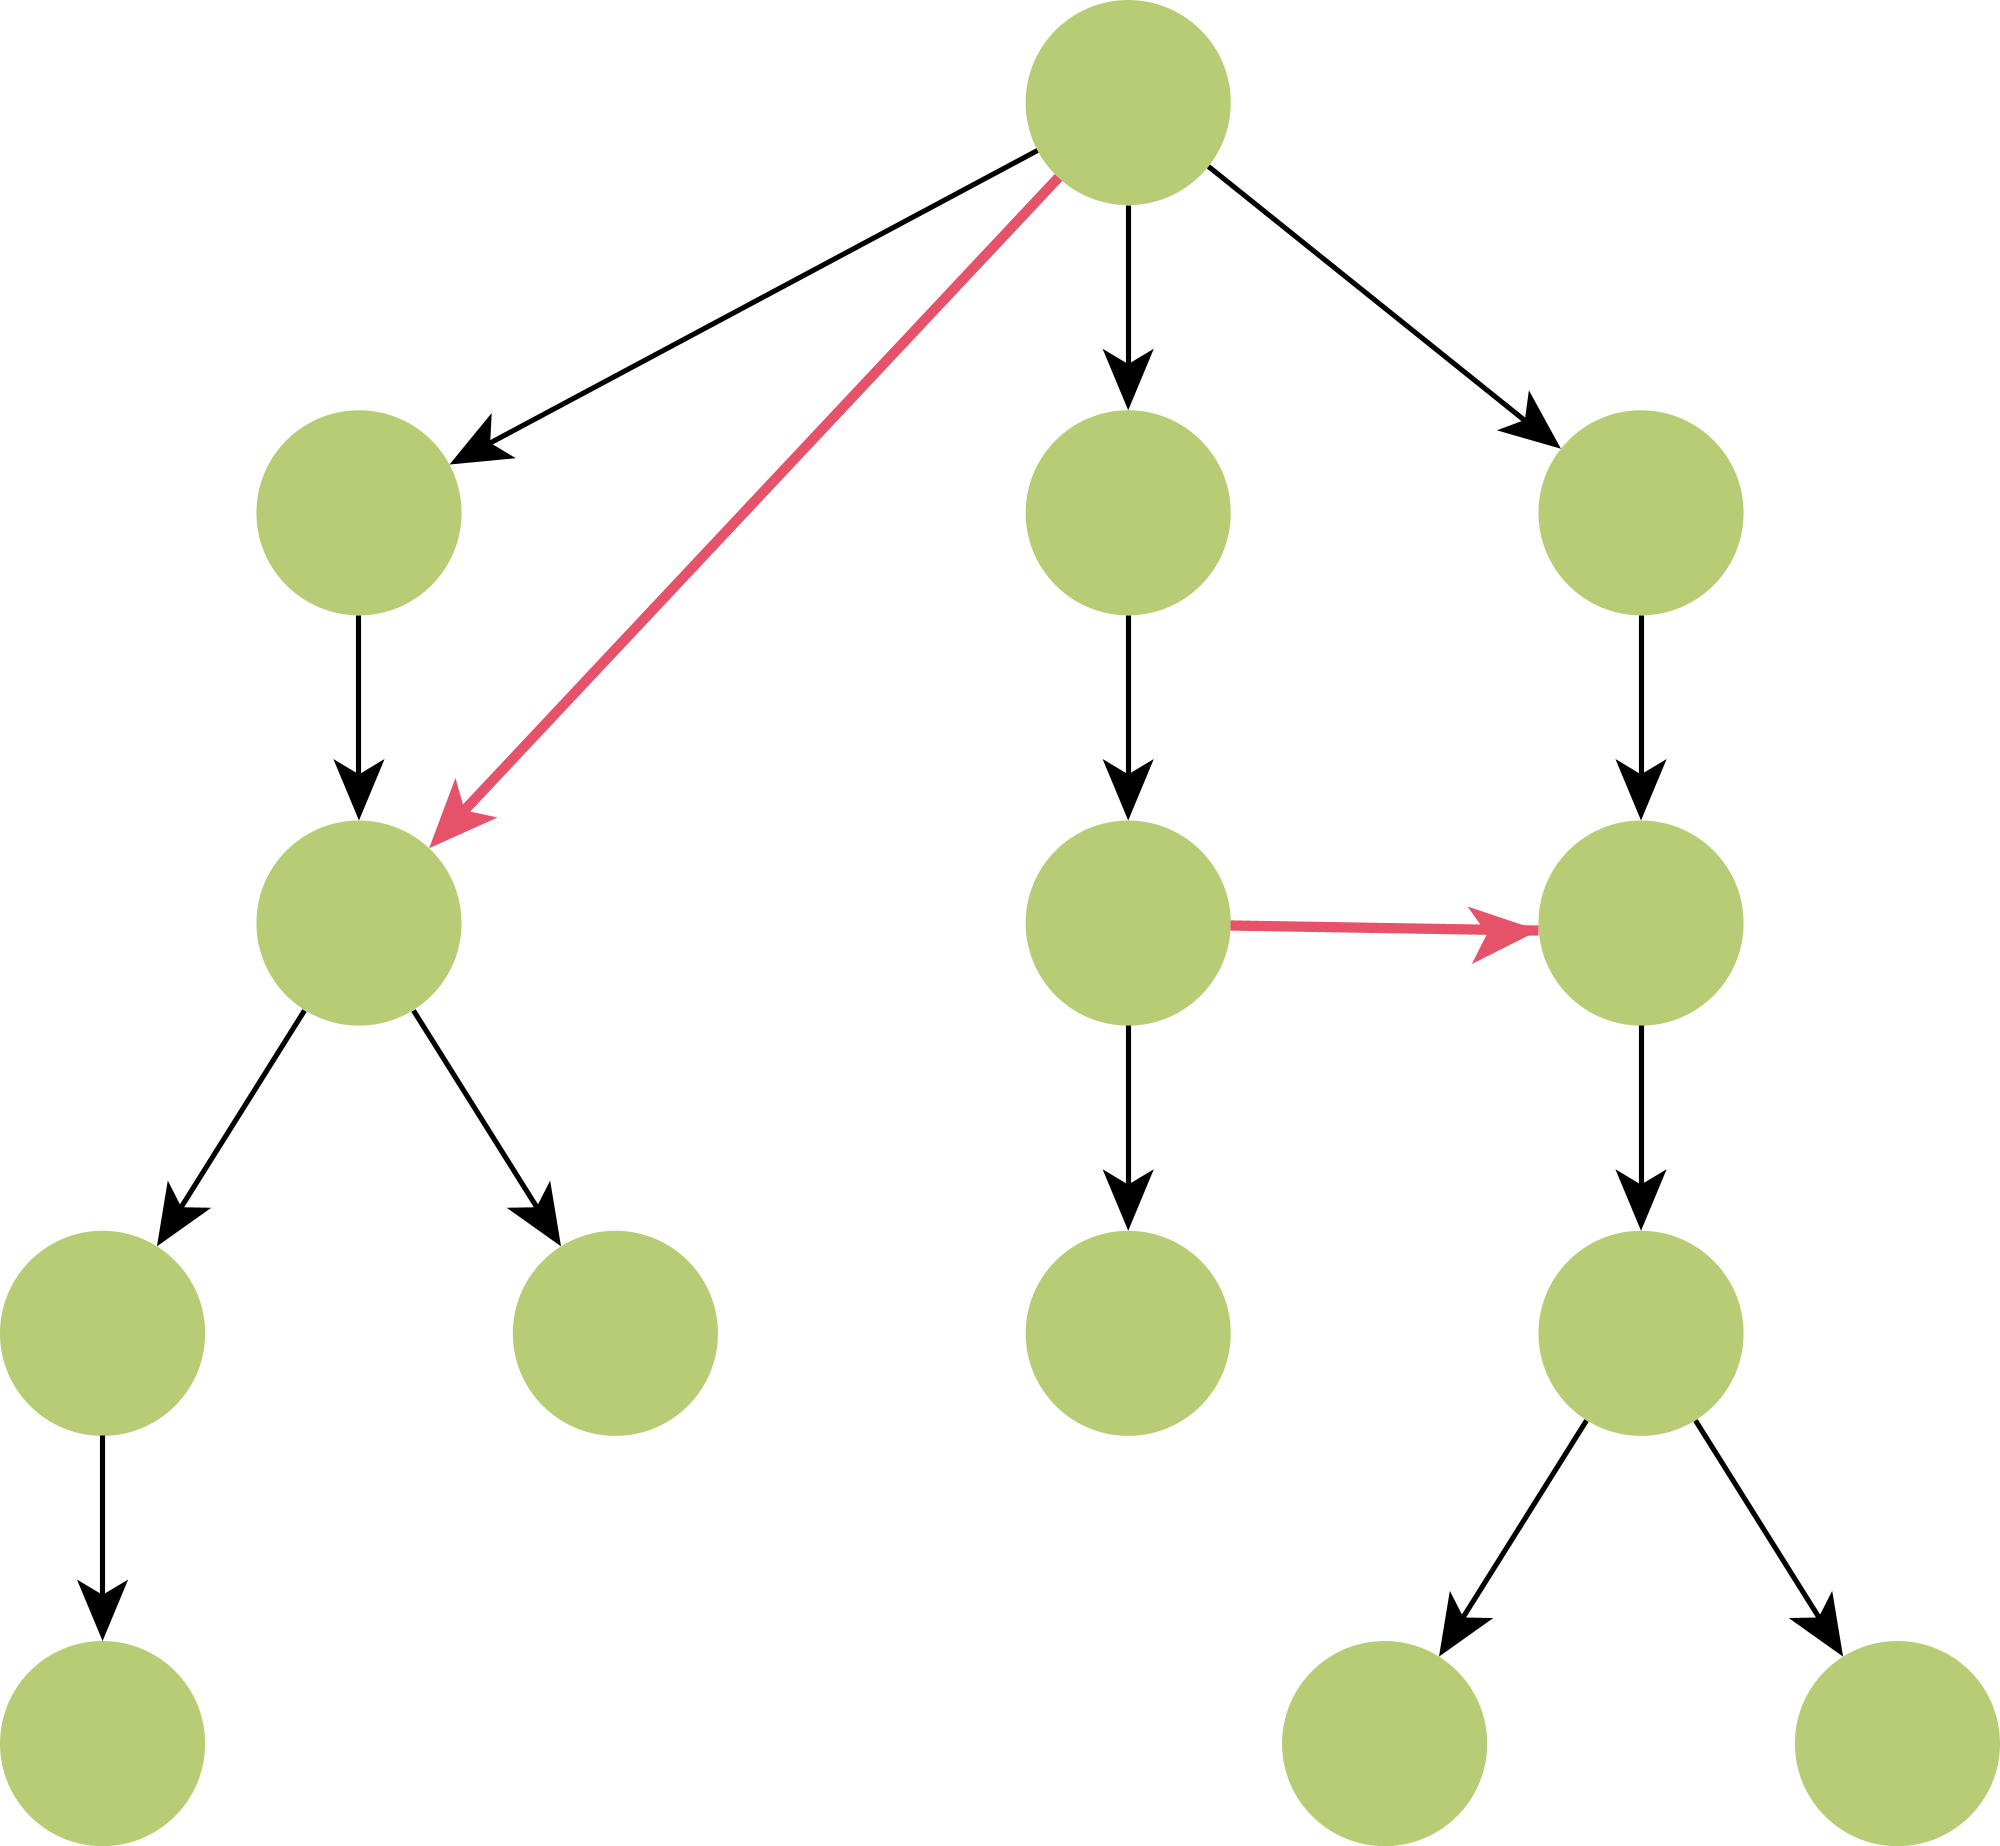
\includegraphics[width=7cm]{graphes2/img/ex_pas_arborescence.png}\\ \footnotesize graphe qui n'en est pas une
        \end{center}
    \end{multicols}
\end{definition}
\begin{exercice}[]
    \begin{center}
        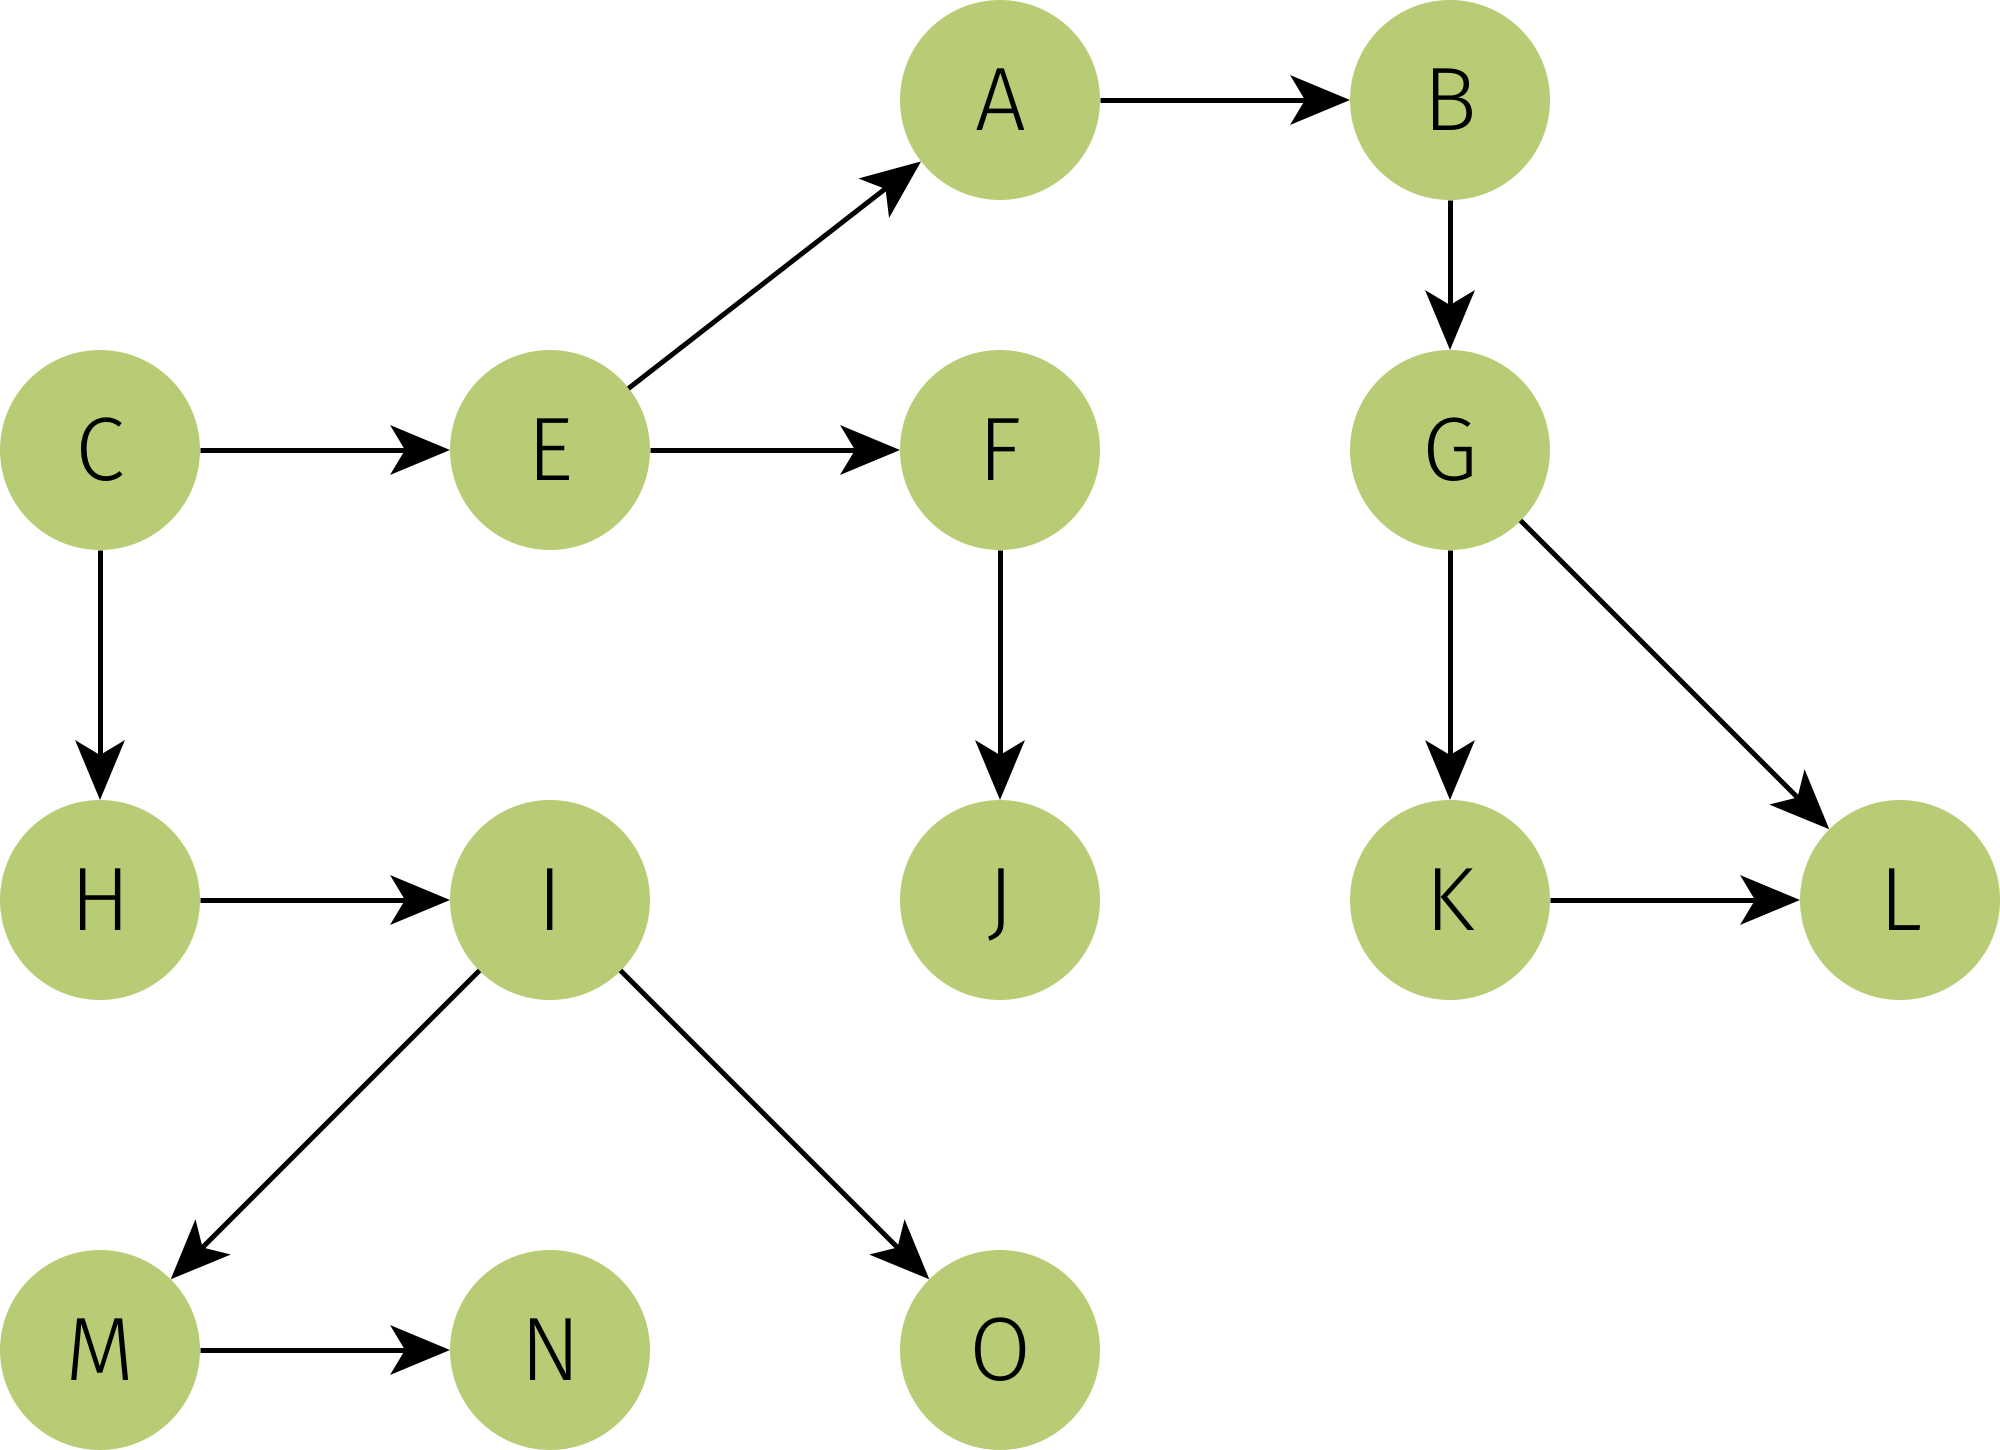
\includegraphics[width=7cm]{graphes2/img/exo_niveau_1.png}
    \end{center}
    \begin{enumerate}
        \item 	Dresser le tableau des prédécesseurs du graphe ci-dessus.
        \item 	Déterminer le niveau de chaque sommet.
        \item 	Dessiner le graphe de manière hiérarchisée.
        \item 	Ce graphe est-il une arborescence ?
    \end{enumerate}
\end{exercice}

\begin{exercice}[]
    \begin{center}
        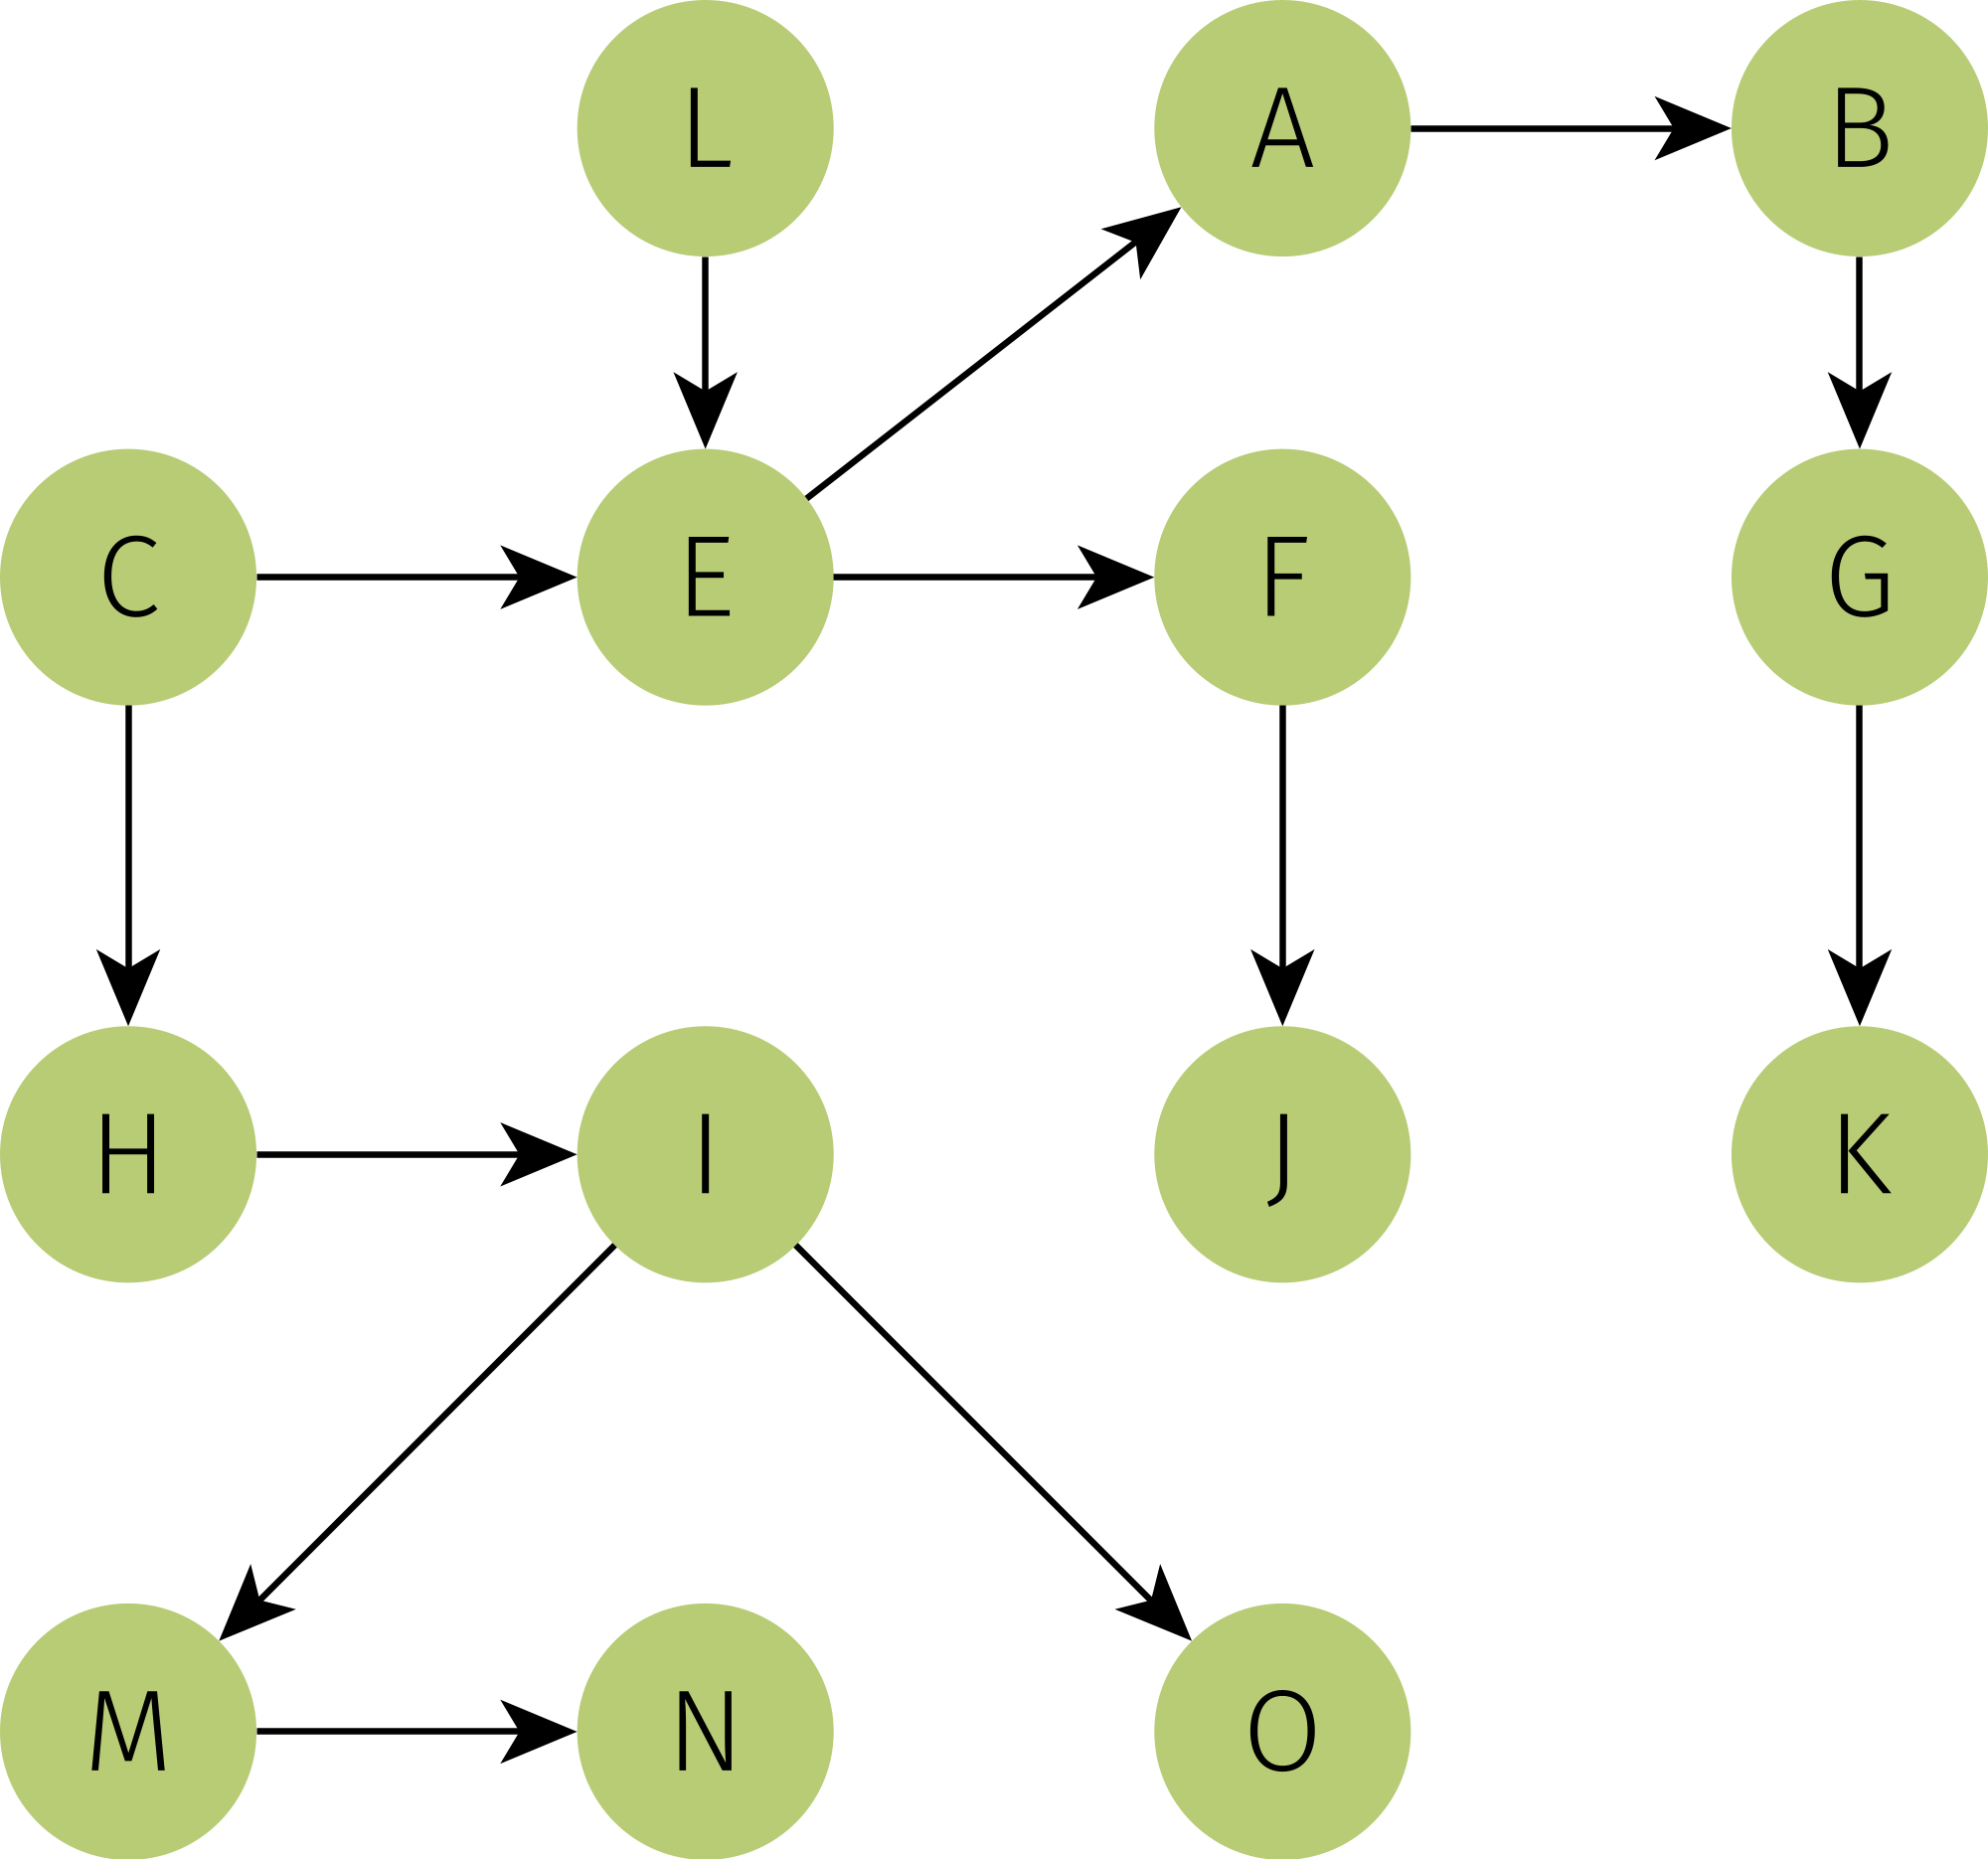
\includegraphics[width=6cm]{graphes2/img/exo_niveau_2.png}
    \end{center}
    Même consigne.
\end{exercice}

\begin{exercice}[]
    \begin{center}
        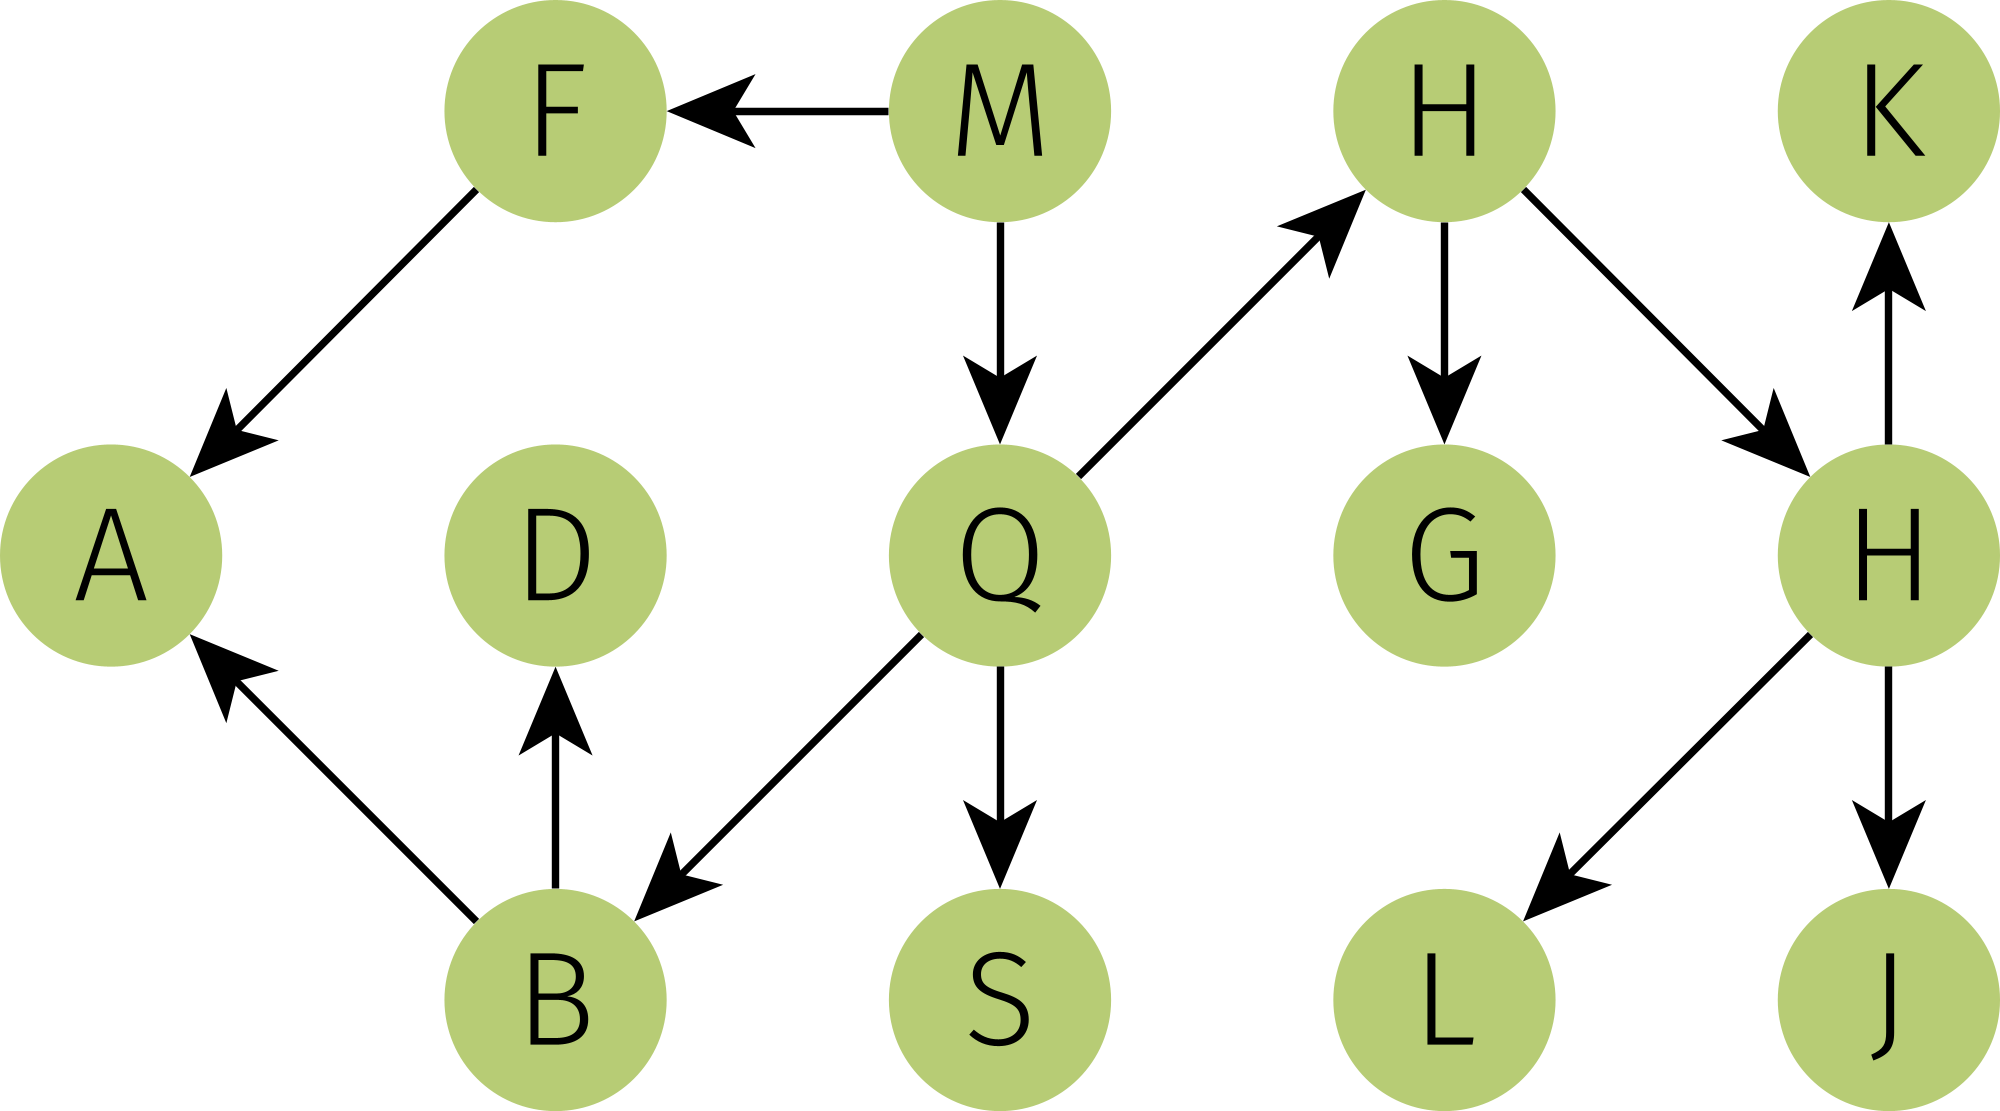
\includegraphics[width=7cm]{graphes2/img/exo_niveau_3.png}
    \end{center}
    Même consigne.
\end{exercice}
\section{Graphes orientés valués et ordonnancement}


\begin{definition}[ : graphe orienté valué]
    un graphe orienté est dit \textit{valué} (on dit aussi pondéré) lorsqu'on attribue un nombre réel à chacun de ses arcs.
    \begin{center}
        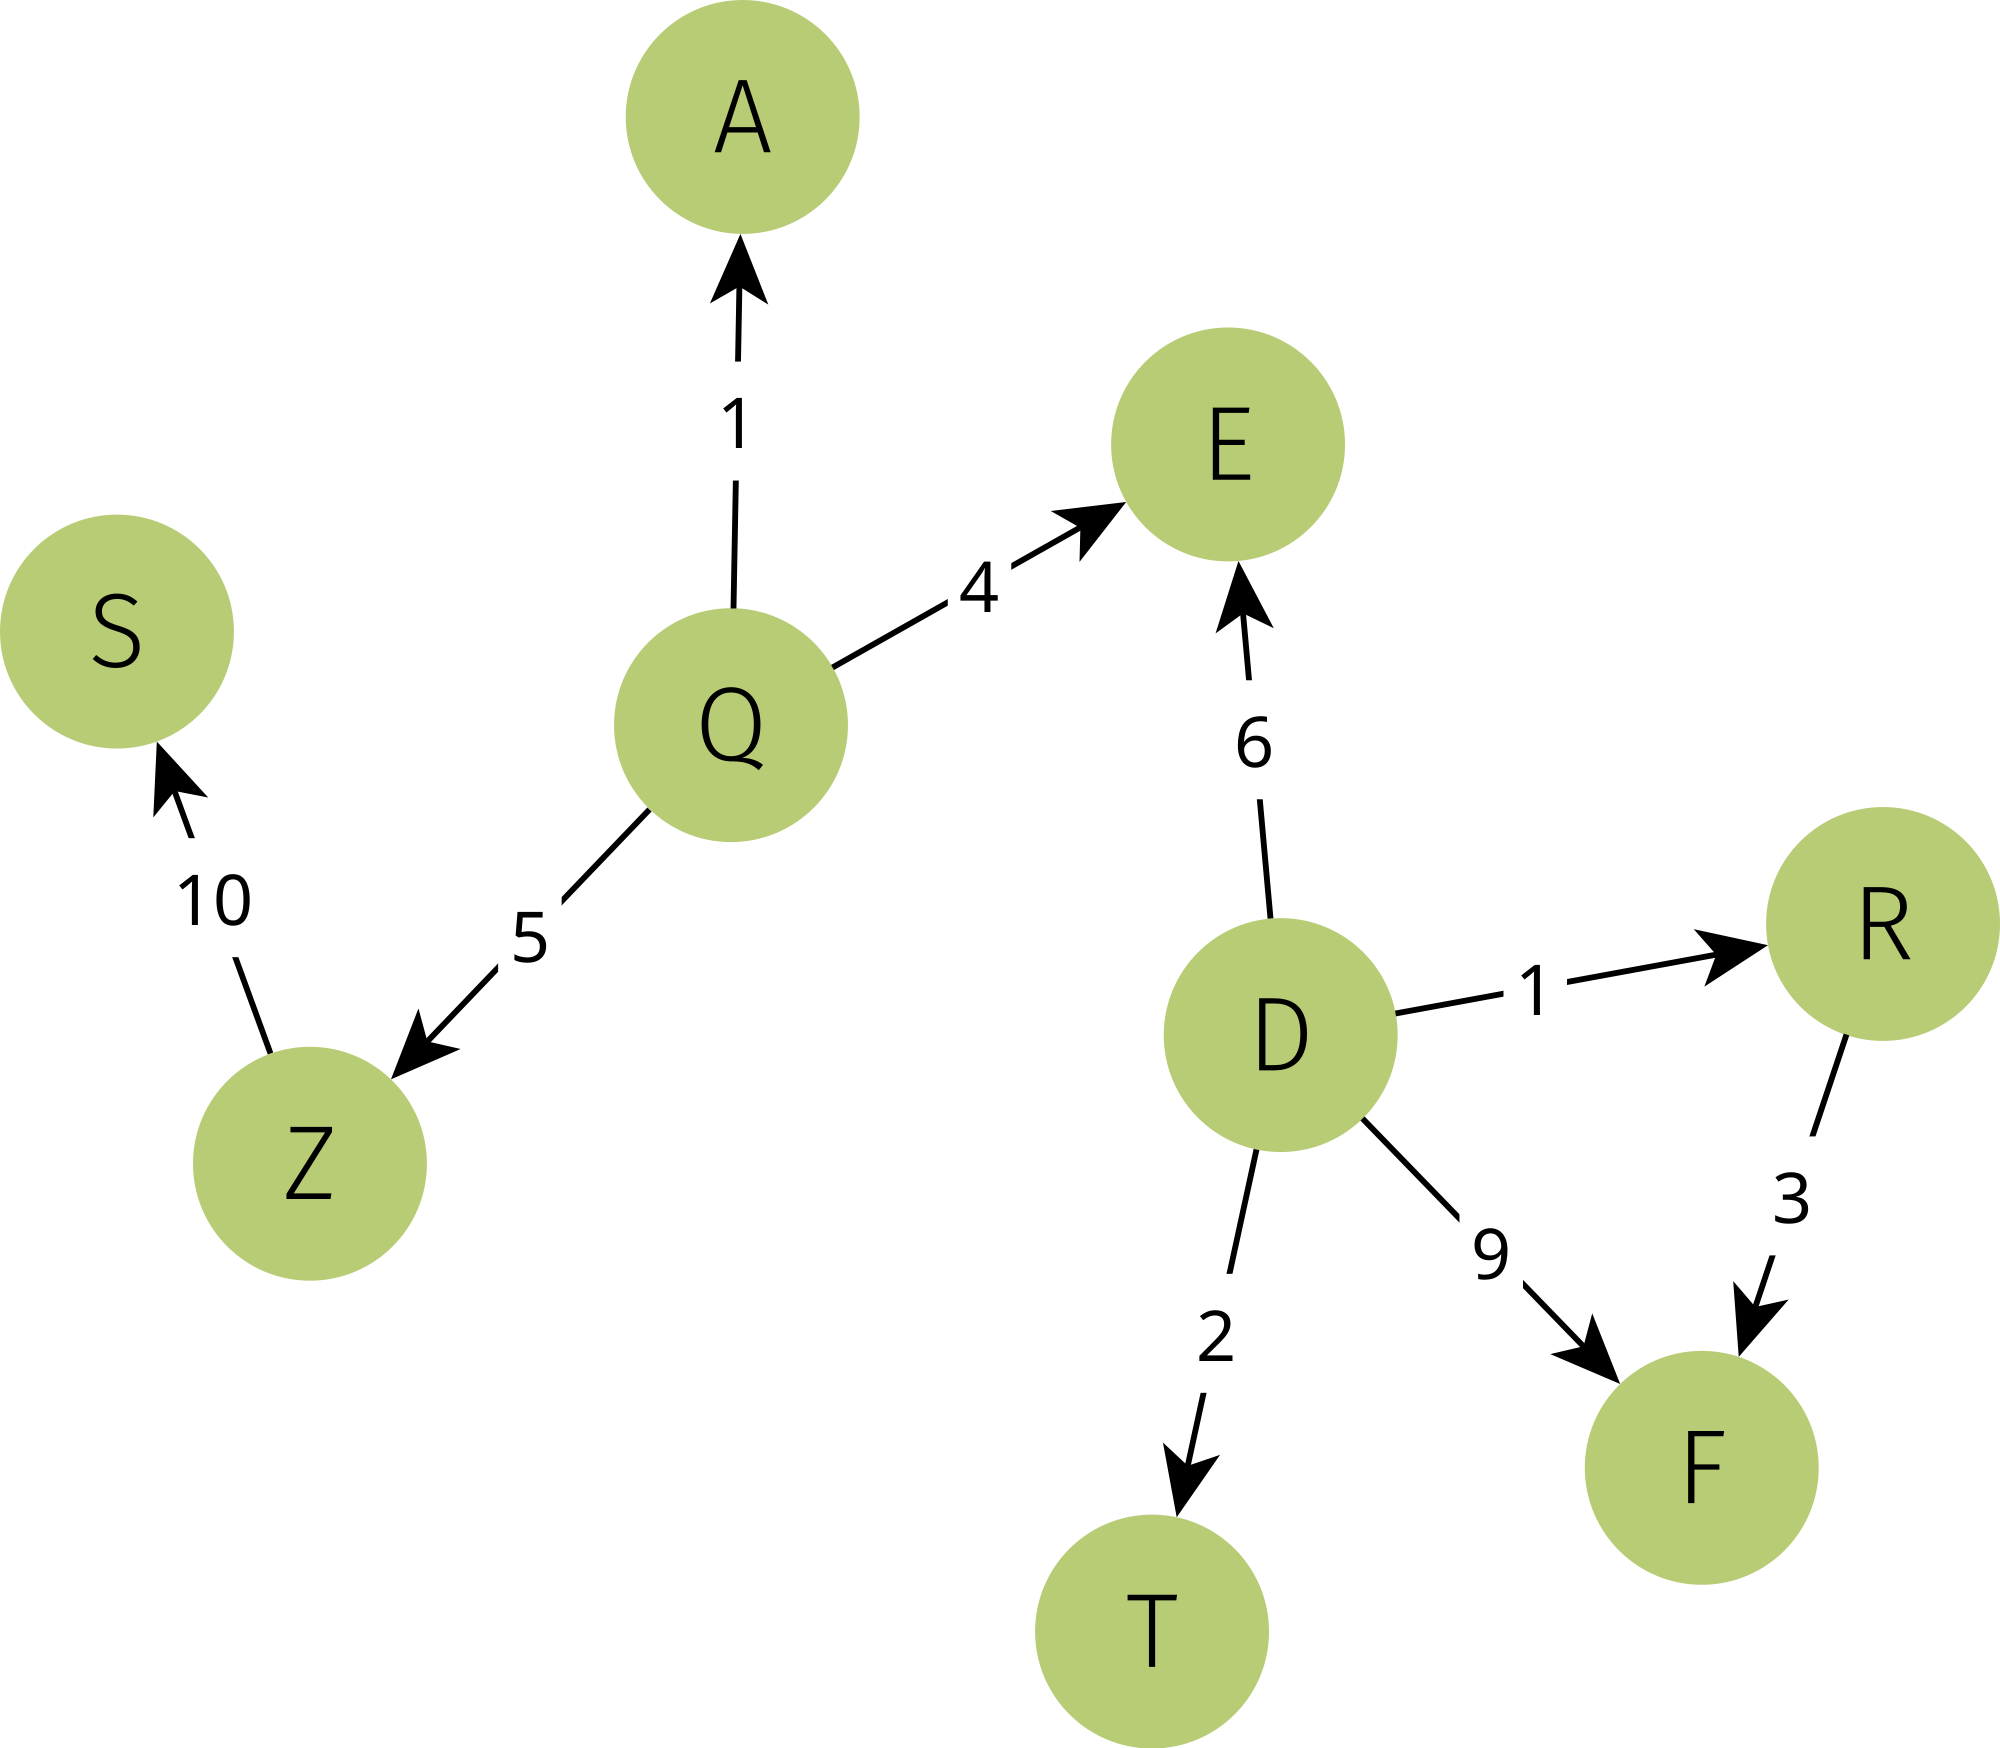
\includegraphics[width=7cm]{graphes2/img/graphe_value.png}\\un exemple de graphe valué
    \end{center}
\end{definition}

Imaginons maintenant une équipe de plusieurs personnes qui travaille sur un projet, (ce peut être le développement d'une application ou bien la construction d'une salle de sport). Toutes les personnes ne travaillent pas sur les mêmes aspects du projet. Certaines tâches peuvent être réalisées en même temps (par exemple on peut penser qu'on peut poser un revêtement au sol de la salle de sport en même temps qu'on peint sa façade). Certaines doivent attendre que d'autres soient terminées pour pouvoir commencer (évidemment avant de peindre la façade il faut avoir monté la façade), on parle de \textit{contraintes d'antériorité}.\\
Les contraintes d'antériorité conduisent naturellement à un graphe orienté. Chaque tâche possède une durée propre, qui conduit à pondérer le graphe.\\

\textit{Faire de l'ordonnancement}, c'est préciser la chronologie des différentes tâches (éventuellement effectuées en parallèle), déterminer la durée minimale du projet et les conséquences éventuelles d'un retard lors de la réalisation de telle ou telle tâche.

\subsection*{La méthode MPM sur un exemple}

Cette méthode de gestion de projet, appelée méthode des potentiels métra (MPM) fut développée par le mathématicien français Bernard Roy en 1958, pour être directement appliquée en usine.\\

On va considérer le tableau de tâches suivant

\begin{center}
    \tabstyle
    \begin{tabular}{lccccccc}
        \hline
        \ccell Tâche              & A   & B   & C   & D & E & F    & G       \\
        \hline
        \ccell Durée en jours     & 6   & 3   & 6   & 2 & 4 & 3    & 1       \\
        \hline
        \ccell Tâches antérieures & --- & --- & --- & B & B & A, D & C, E, F \\
        \hline
    \end{tabular}\\
\end{center}
Dans celui-ci on lit, par exemple, que la tâche F dure 3 jours et ne peut commencer que lorsque A et D sont terminées.\\


Cet exemple va nous servir à illustrer la méthode MPM, mais nous donnerons les définitions dans le cas général.

\begin{encadrecolore}{Notations}{UGLiPurple}
    On note $G$ le graphe orienté valué qui représente les tâches du projet.\\
    Il a $n$ sommets $s_1$, ..., $s_n$ qui représentent toutes les tâches. On écrit $s_i$ pour parler d'un de ces sommets sans dire précisément lequel.\\
    On note aussi $d(s_i)$ la durée de la tâche $s_i$, c'est la valeur (le poids) de tous les arcs qui partent de $s_i$.
\end{encadrecolore}



\subsubsection*{Niveler le graphe}

Dans le graphe qu'on va construire, les tâches antérieures sont les \textit{prédécesseurs directs} de chaque tâche, et il n'y a pas de circuit (heureusement pour le projet). On peut donc niveler le graphe :
\begin{itemize}
    \item 	A, B et C sont clairement de niveau 0;
    \item 	D et E sont de niveau 1;
    \item 	F est de niveau 2;
    \item 	G est de niveau 3.
\end{itemize}
Cela nous permet de représenter le graphe du projet de manière hiérarchisée. On parle alors de \textit{graphe d'ordonnancement}. Pour les besoins on rajoute 2 sommets « fictifs»{} : le début et la fin du projet. On pondère les arcs par les durées des tâches (on met 0 en partant de début car on considère que le projet peut commencer maintenant) :
\begin{center}
    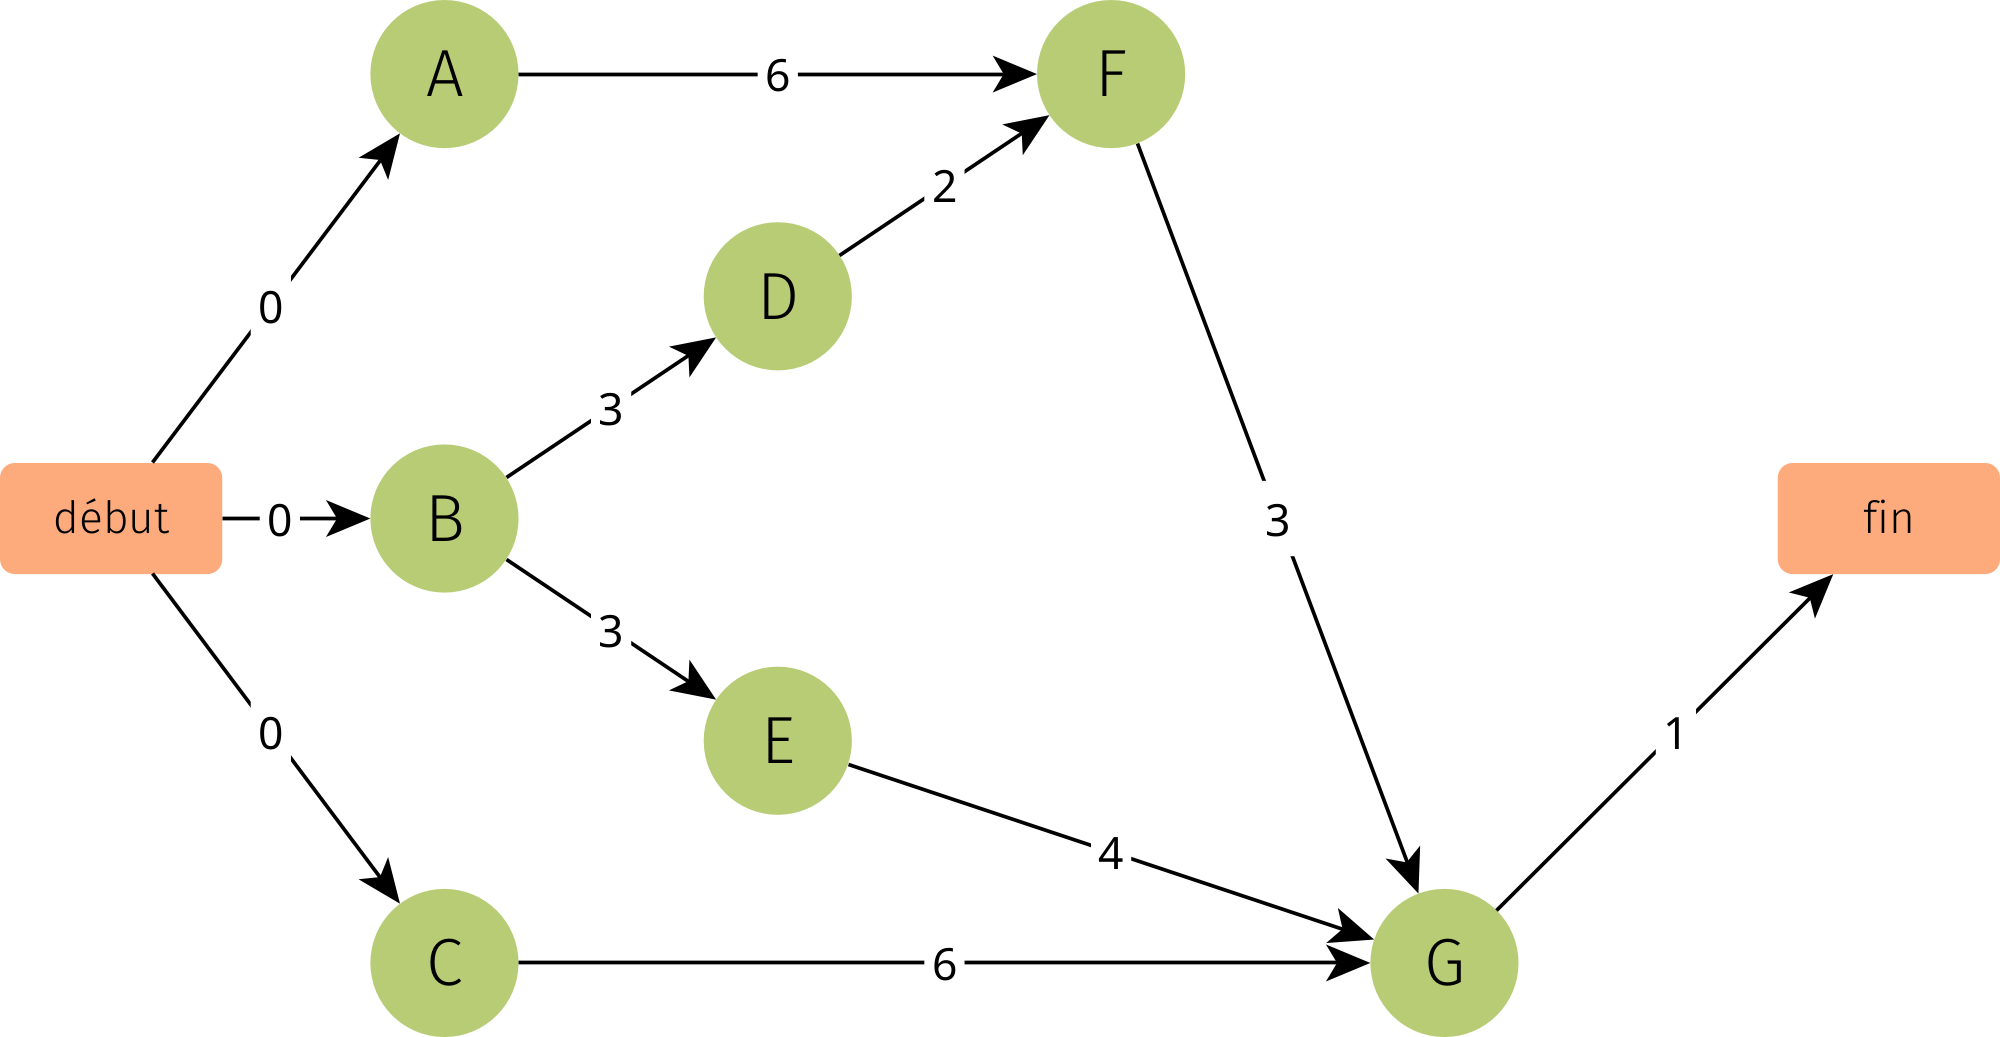
\includegraphics[width=12cm]{graphes2/img/exemple_mpm0.png}
\end{center}
Puis, étant donné que l'on va déterminer beaucoup de paramètres, on utilisera plutôt cette représentation :
\begin{center}
    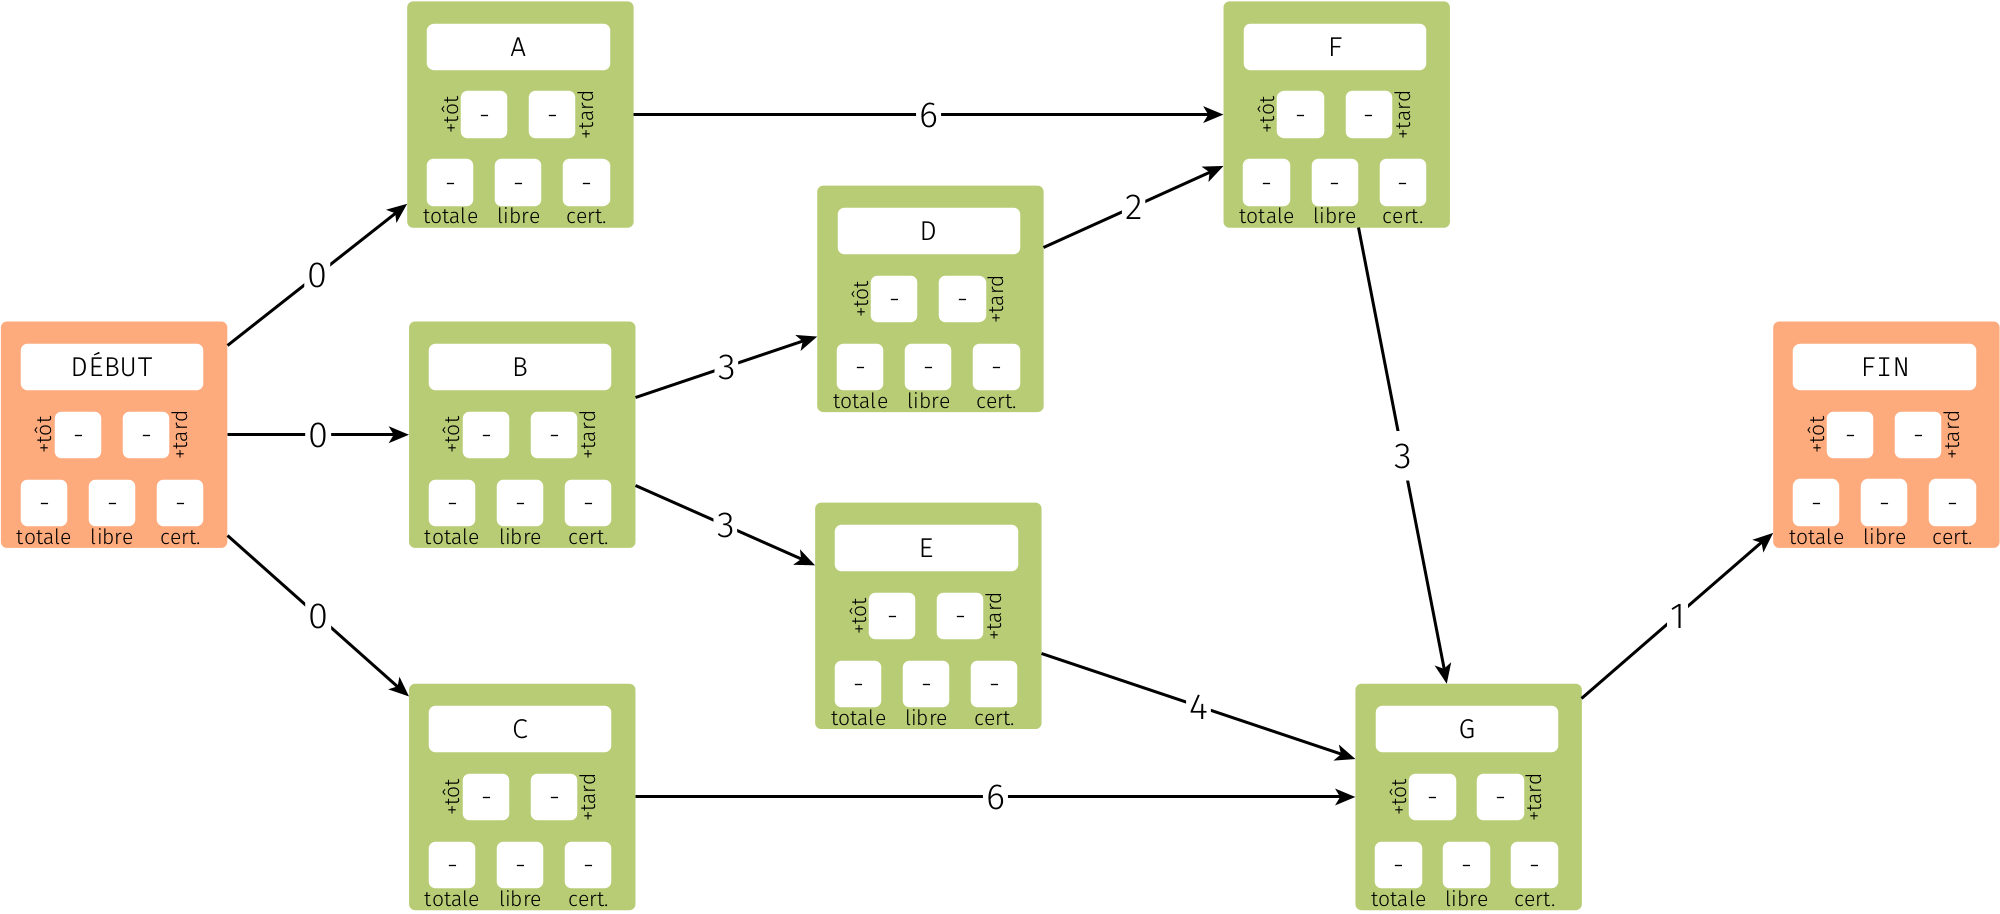
\includegraphics[width=\linewidth]{graphes2/img/exemple_mpm1.png}
\end{center}
Comme on peut le voir, pour chaque sommet, on peut déterminer 5 paramètres :\\

\dleft{4cm}{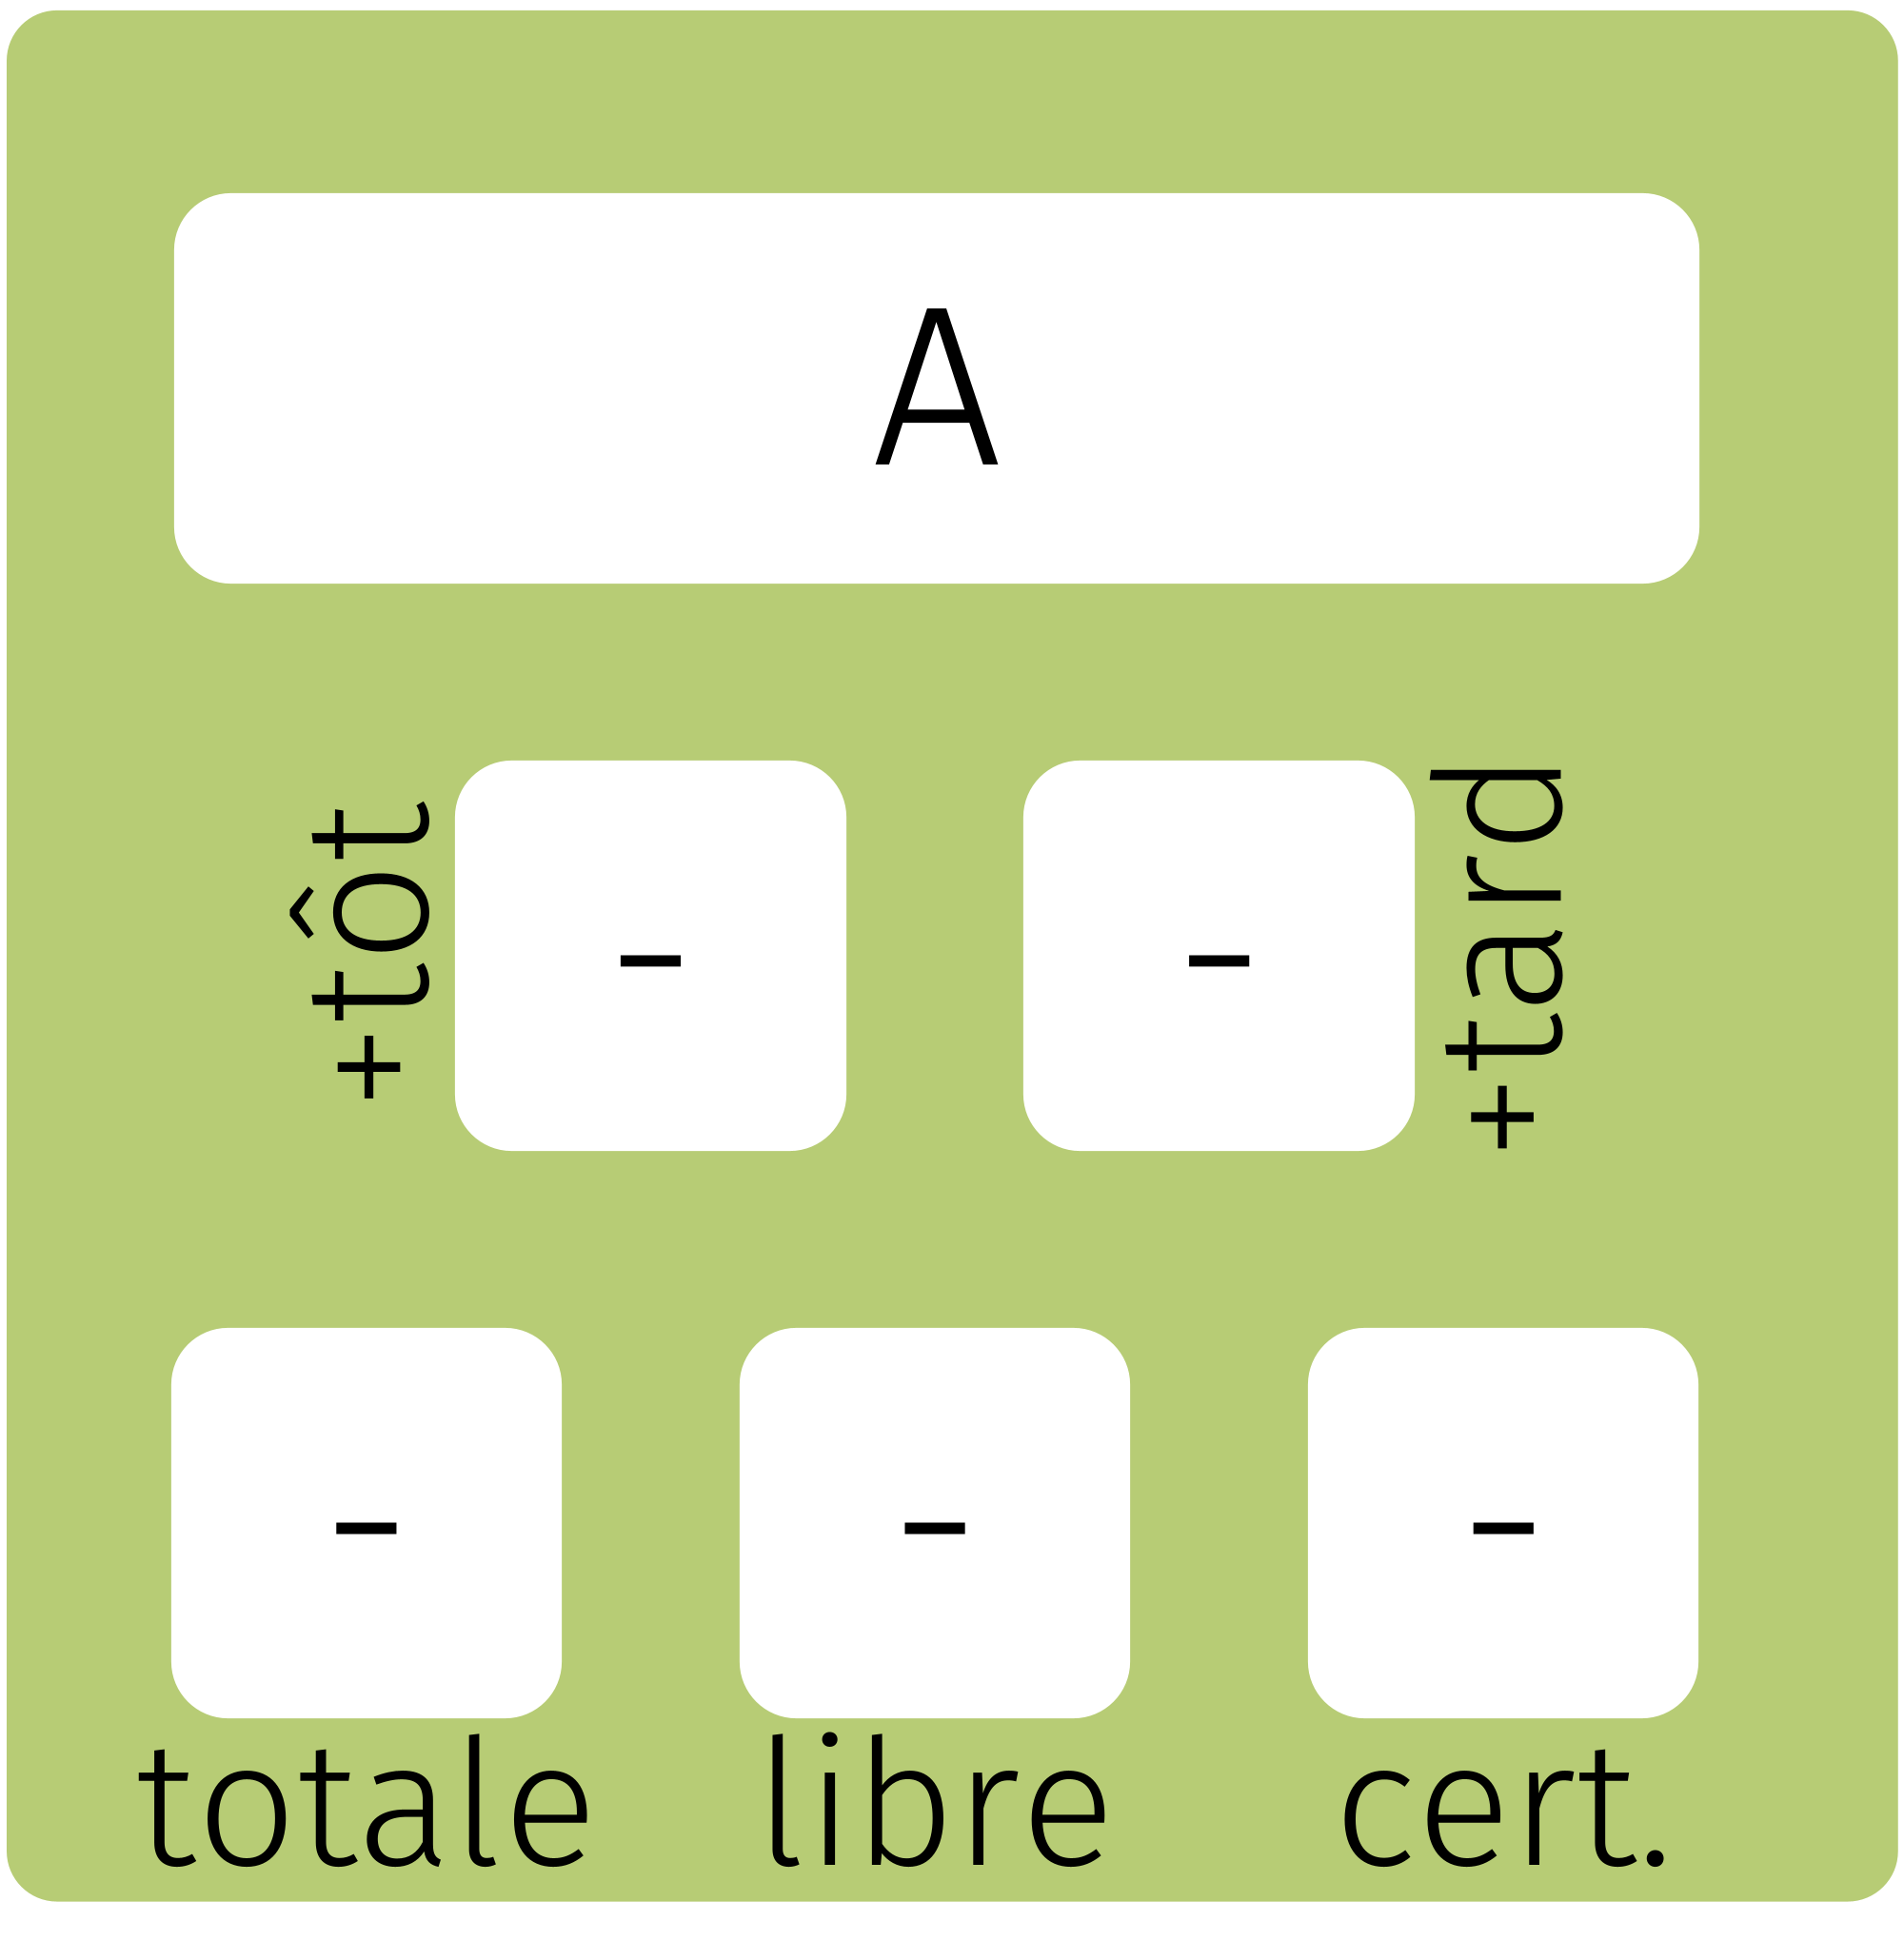
\includegraphics[width=4cm]{graphes2/img/sommet_template.png}}{\begin{enumerate}
        \item 	D'abord, on détermine la \textit{date au plus tôt} de chaque tâche.
        \item 	Ensuite on peut déterminer la \textit{date au plus tard} de chaque tâche.
        \item 	Cela permet de déterminer la \textit{marge totale} de chaque tâche, ainsi que la \textit{marge libre} et la \textit{marge certaine}.
    \end{enumerate}Nous allons définir ces nombres au fur et à mesure.}

\subsubsection*{Date au plus tôt}

\begin{definition}[ : date au plus tôt]
    On note $t(s_i)$ la \textit{date au plus tôt} de la tâche $s_i$. Puisque $s_i$ ne peut commencer que lorsque toutes les tâches antérieures sont terminées on a
    $$t(s_i)=\max\left(\left\{t(s_j)+d(s_j)\::\:s_j\,\text{ prédécesseur de }\:s_i\right\}\right)$$
\end{definition}
\begin{exemple}[]
    \begin{center}
        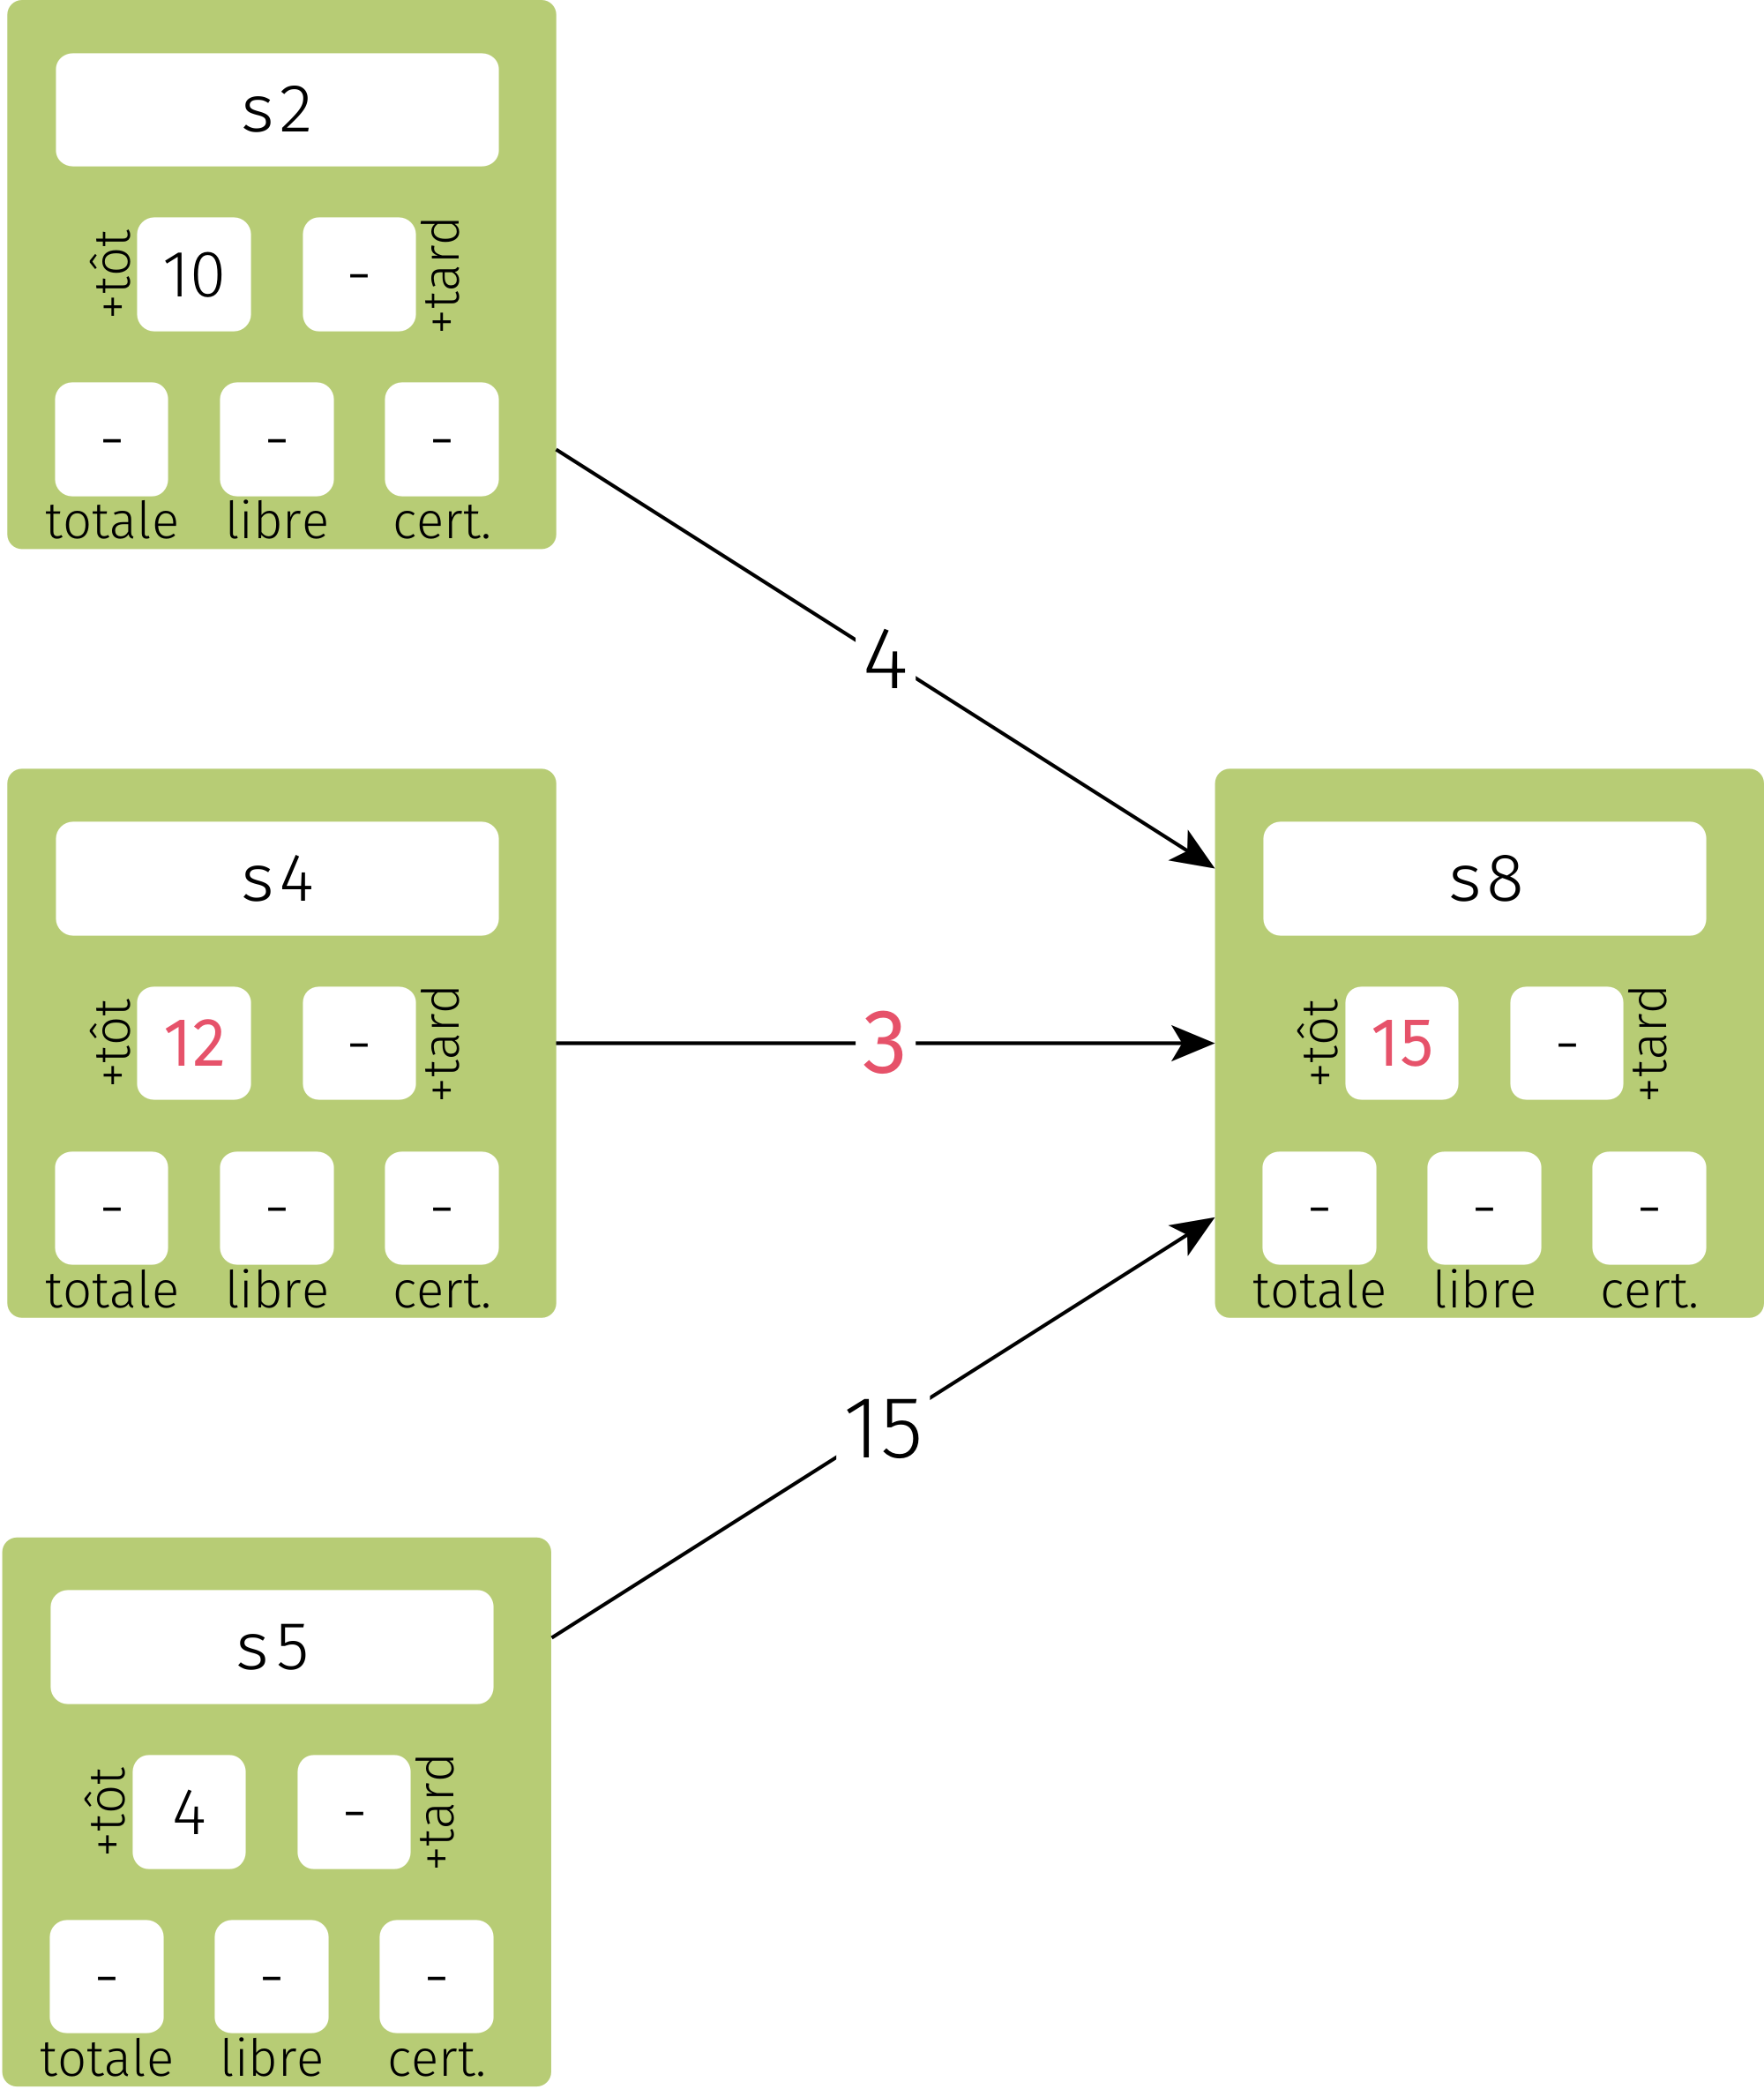
\includegraphics[width=5.5cm]{graphes2/img/mpm_au_plus_tot.png}
    \end{center}
    Pour calculer la date au plus tôt de $s_8$, il faut que les tâches antérieures $s_2$, $s_4$ et $s_5$ soient terminées :
    \begin{itemize}
        \item 	$s_2$ commence au bout de 10 jours, dure 4 jours, donc est terminée au bout de 14 jours;
        \item 	$s_4$ commence au bout de 12 jours, dure 3 jours, donc est terminée au bout de 15 jours;
        \item 	$s_5$ commence au bout de 4 jours,  dure 10 jours, donc est terminée au bout de 14 jours.
    \end{itemize}
    En définitive, $t(s_8)=15$.
\end{exemple}

Calculons toutes les dates au plus tôt de notre projet. On commence par le début et on procède \textit{niveau par niveau} dans l'ordre hiérarchique :
\begin{center}
    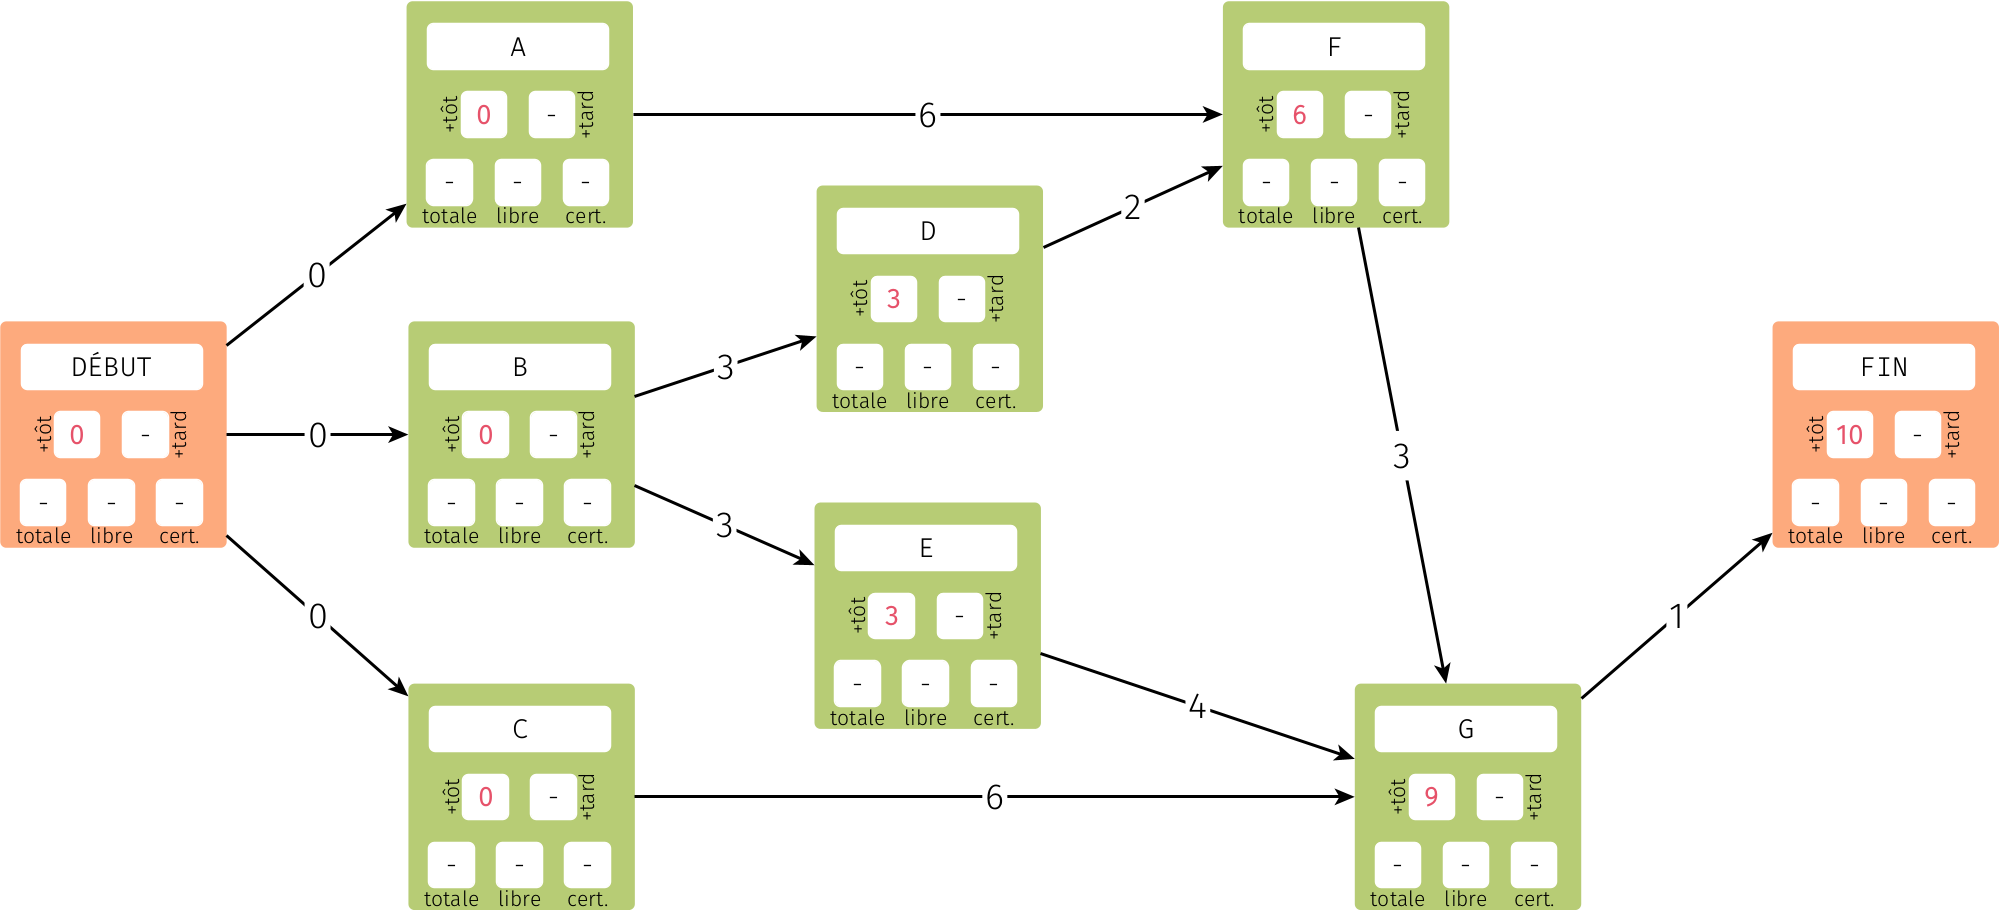
\includegraphics[width=\linewidth]{graphes2/img/exemple_mpm2.png}
\end{center}
\begin{definition}[ : durée minimale de réalisation d'un projet]
    C'est le temps minimal requis pour que toutes les tâches soient accomplies en respectant les contraintes.
\end{definition}
Dans notre cas la \textit{durée minimale du projet} est de 10 jours.

\subsubsection*{Date au plus tard}

\begin{definition}[ : date au plus tard]
    On note $T(s_i)$ la \textit{date au plus tard} de la tâche $s_i$ : c'est la date maximale à laquelle on peut commencer $s_i$ sans que cela ne repousse la date de fin du projet.
    $$T(s_i)=\min\left(\left\{T(s_j)-d(s_i)\::\:s_j\,\text{ successeur de }\:s_i\right\}\right)$$
\end{definition}
\begin{exemple}[]
    \begin{center}
        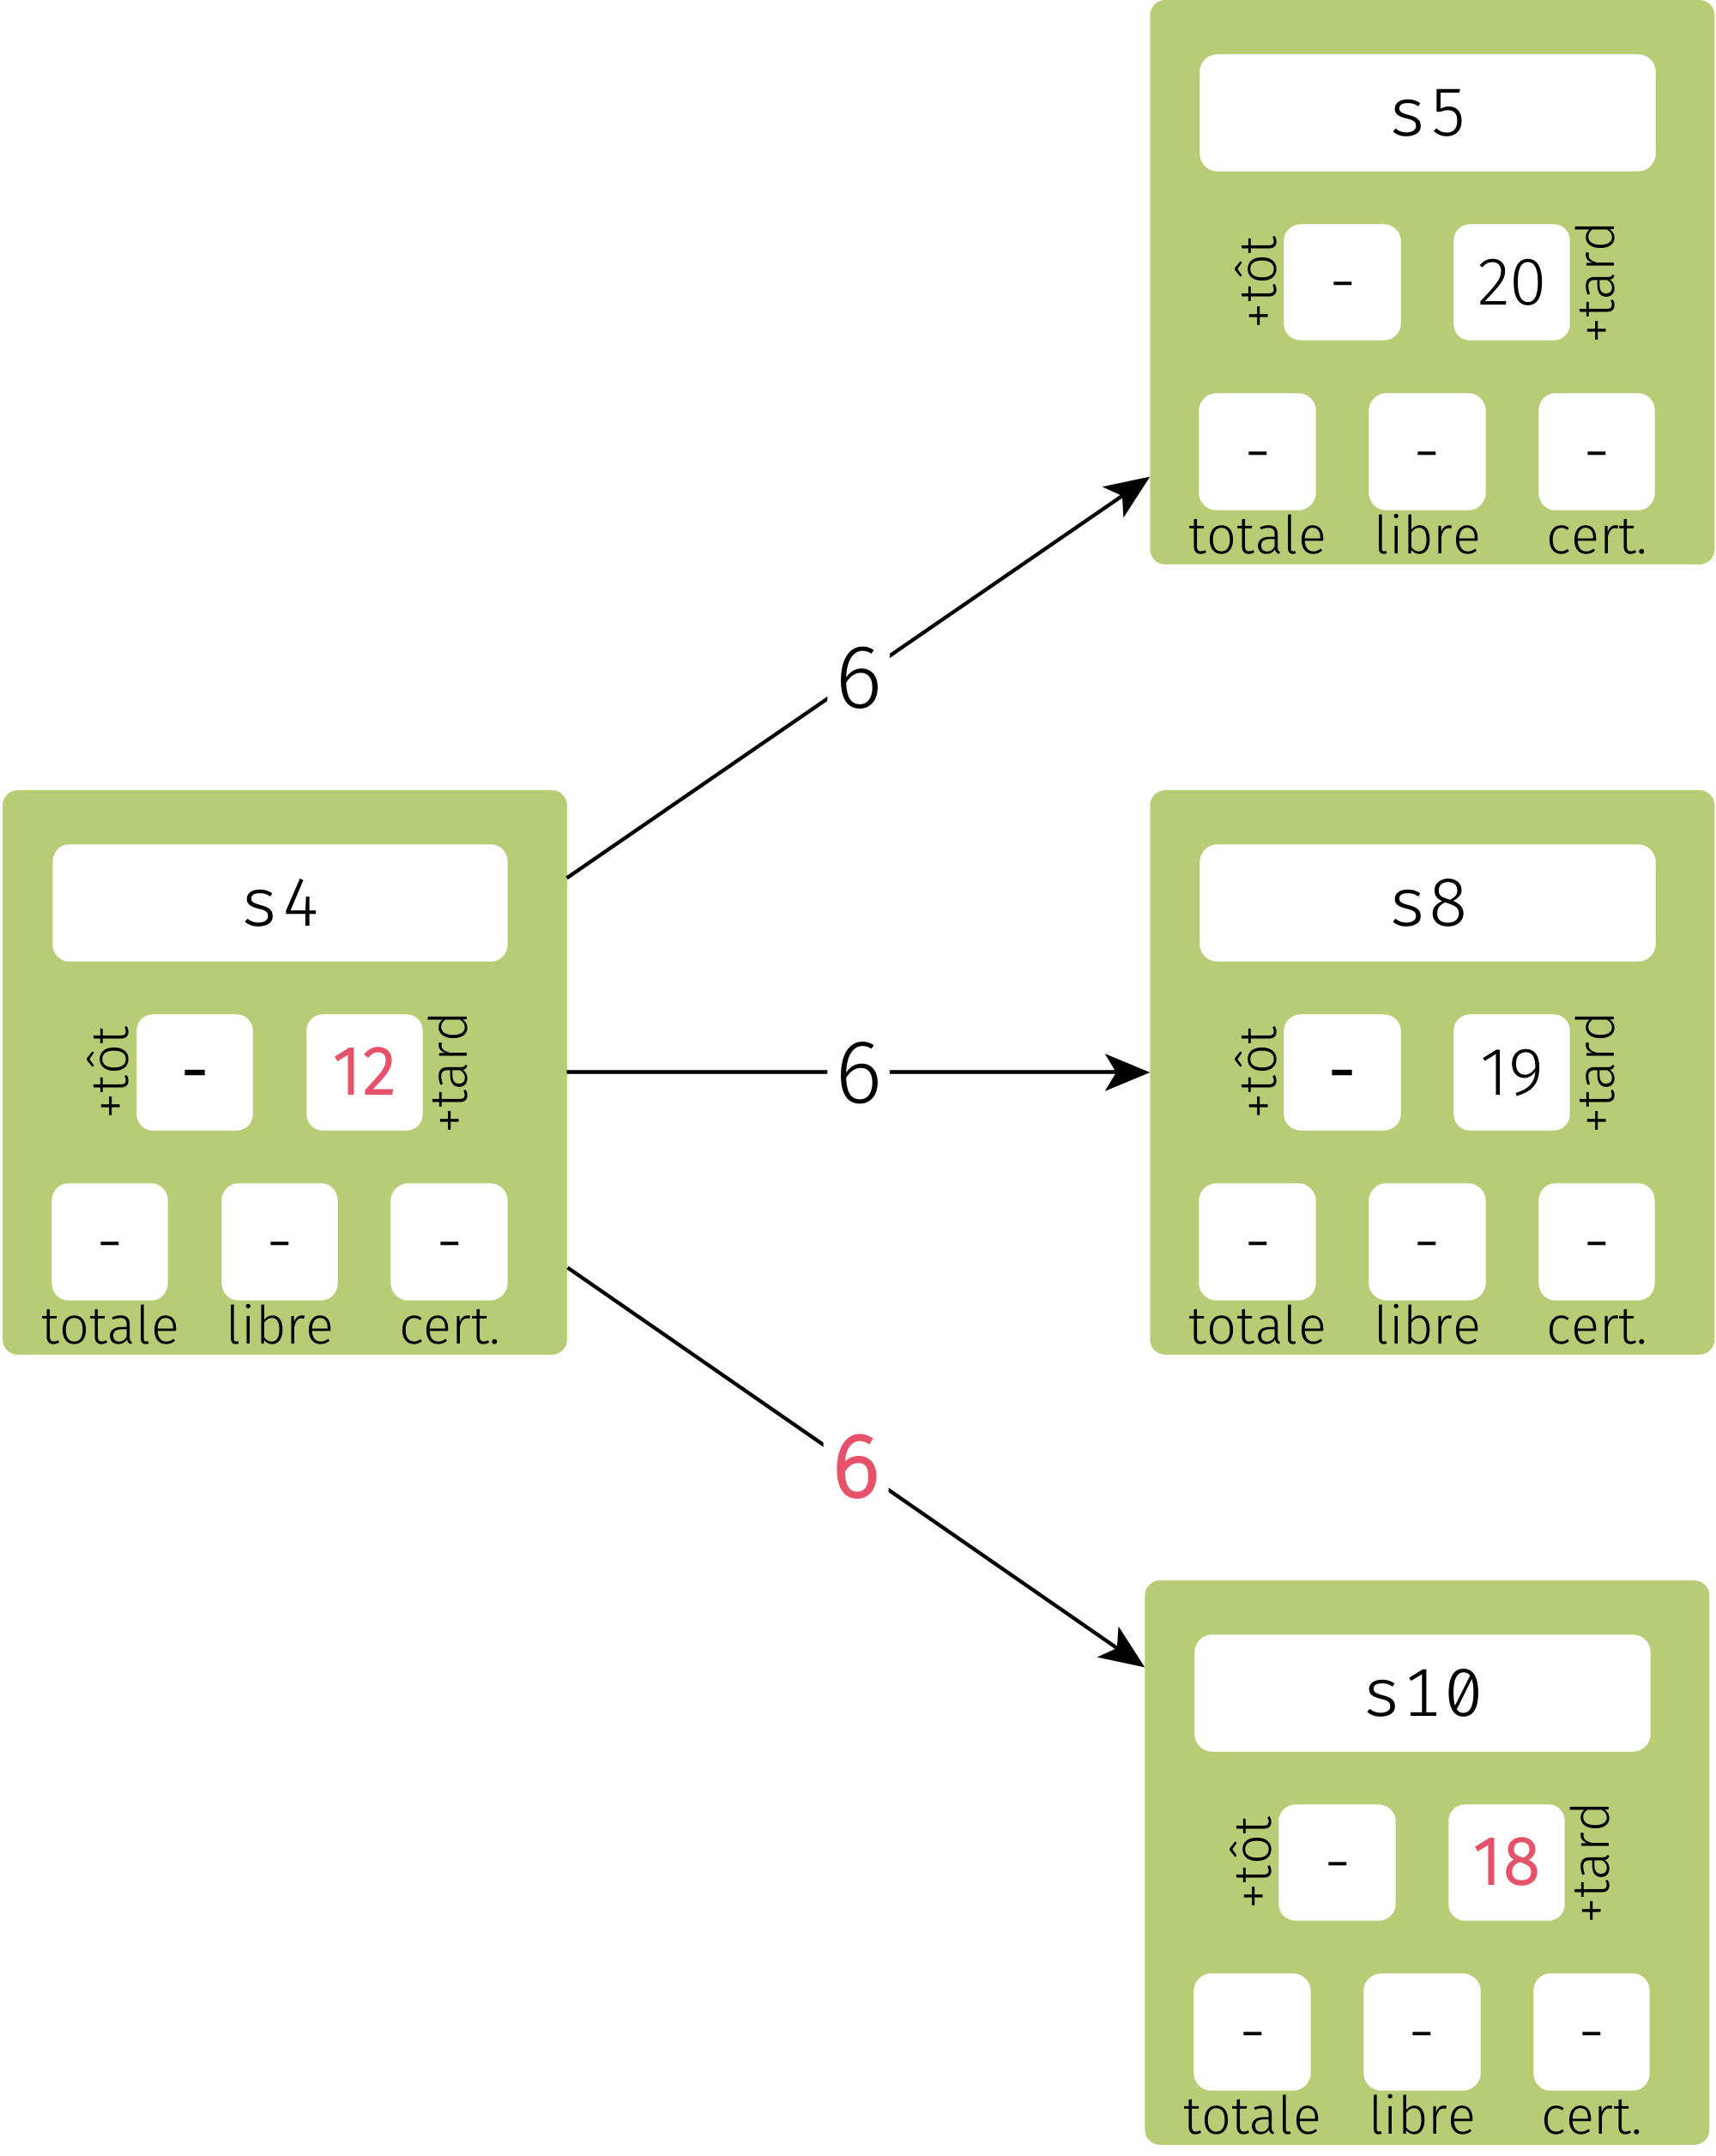
\includegraphics[width=5.5cm]{graphes2/img/mpm_au_plus_tard.png}
    \end{center}
    On n'a pas renseigné les dates au plus tôt car elles n'interviennent pas ici, mais normalement elles doivent avoir été calculées d'abord.\\
    La tâche $s_4$ dure 6 jours
    \begin{itemize}
        \item 	puisqu'on peut commencer $s_5$ au plus tard au bout de 20 jours, il faut commencer $s_4$ au plus tard au bout de $20-6=14$ jours pour ne pas ralentir;
        \item 	Puisqu'on peut commencer $s_8$ au plus tard au bout de 19 jours, il faut commencer $s_4$ au plus tard au bout de $19-6=13$ jours pour ne pas ralentir;
        \item 	Puisqu'on peut commencer $s_{10}$ au plus tard au bout de 18 jours, il faut commencer $s_4$ au plus tard au bout de $18-6=12$ jours pour ne pas ralentir.
    \end{itemize}
    Ainsi $T(s_4)=12$.
\end{exemple}
Calculons toutes les dates au plus tard de notre projet. On commence par la fin : la date au plus tard de la fin est par définition égale à sa date au plus tôt. Ensuite on « remonte»{} la hiérarchie niveau par niveau :
\begin{center}
    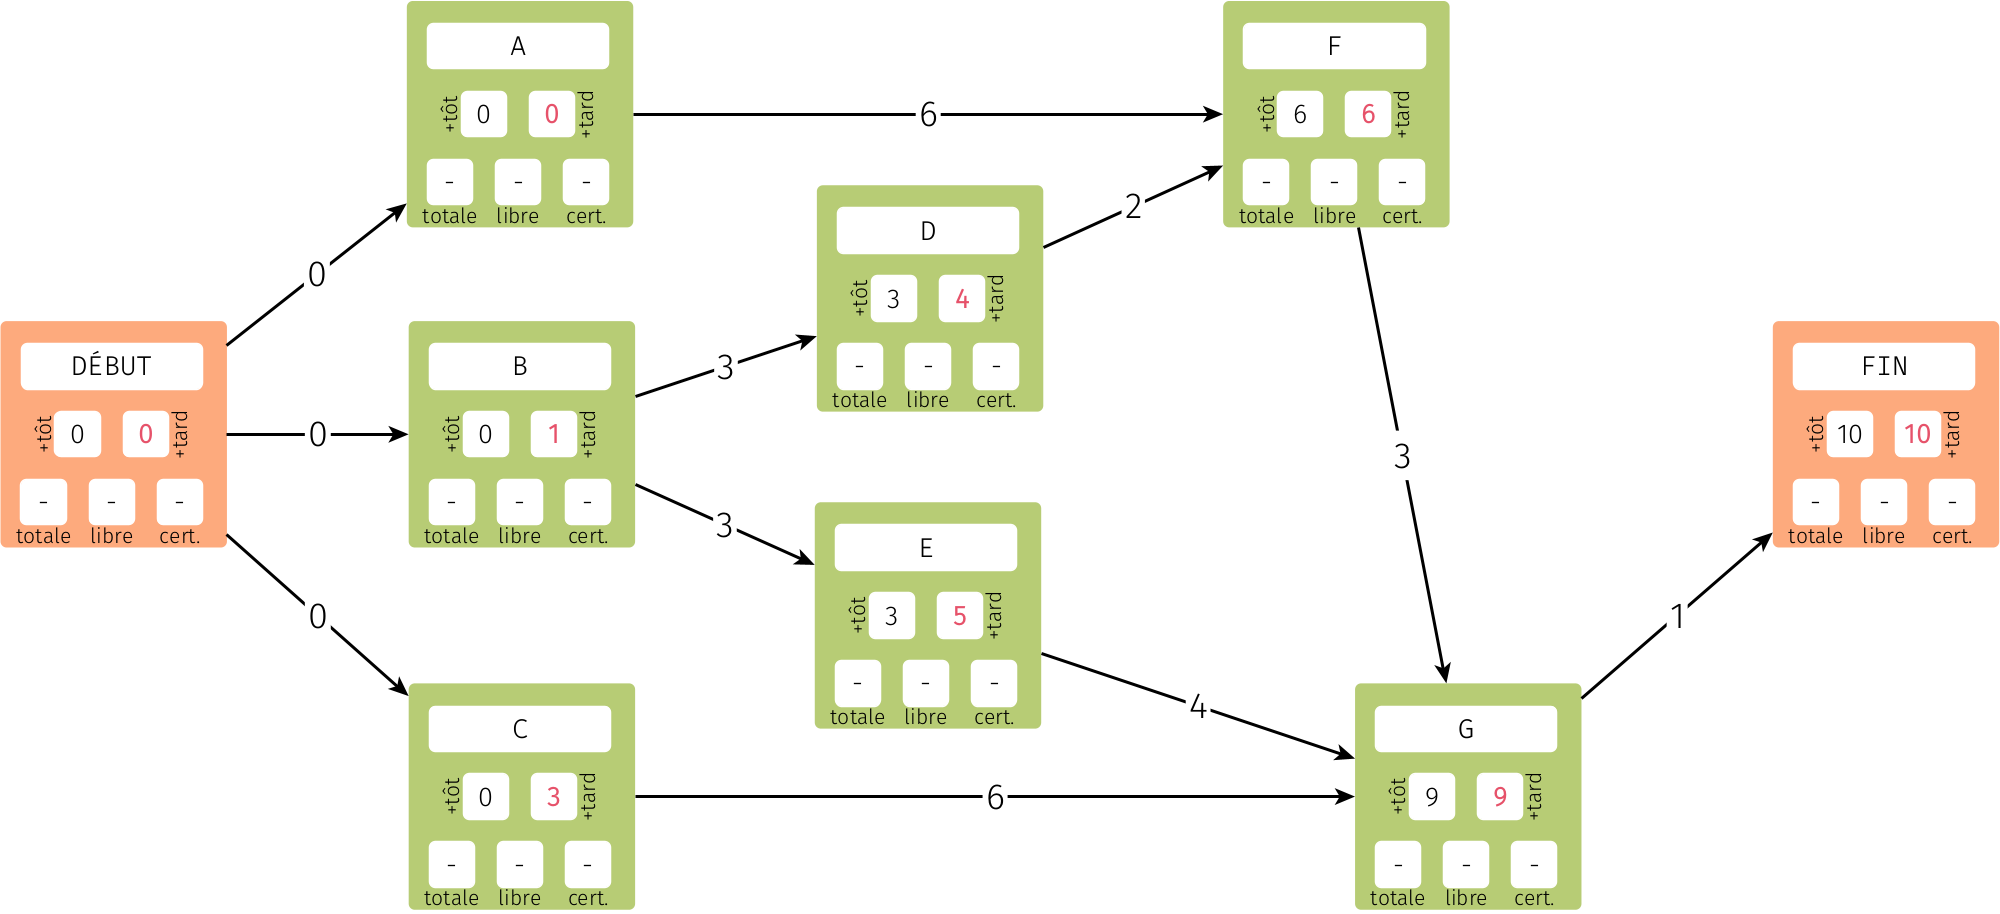
\includegraphics[width=\linewidth]{graphes2/img/exemple_mpm3.png}
\end{center}
On s'aperçoit que certaines tâches autorisent une « marge de man\oe uvre»{} et d'autres non. Nous allons préciser cela.
\subsubsection*{Marge totale, tâche critique}
\begin{definition}[s : marge totale et tâche critique]
    La \textit{marge totale} d'une tâche $s_i$ est $$MT(s_i)=T(s_i)-t(s_i)$$
    C'est le retard maximum que l'on peut accepter sur la date de début au plus tôt de la tâche sans que cela ne retarde la date de fin de projet.\\

    Si la marge totale d'une tâche est nulle, on dit que c'est une \textit{tâche critique} : on doit impérativement la commencer au plus tôt, sinon le projet sera ralenti.
\end{definition}

\begin{exemple}[]
    \dleft{4cm}{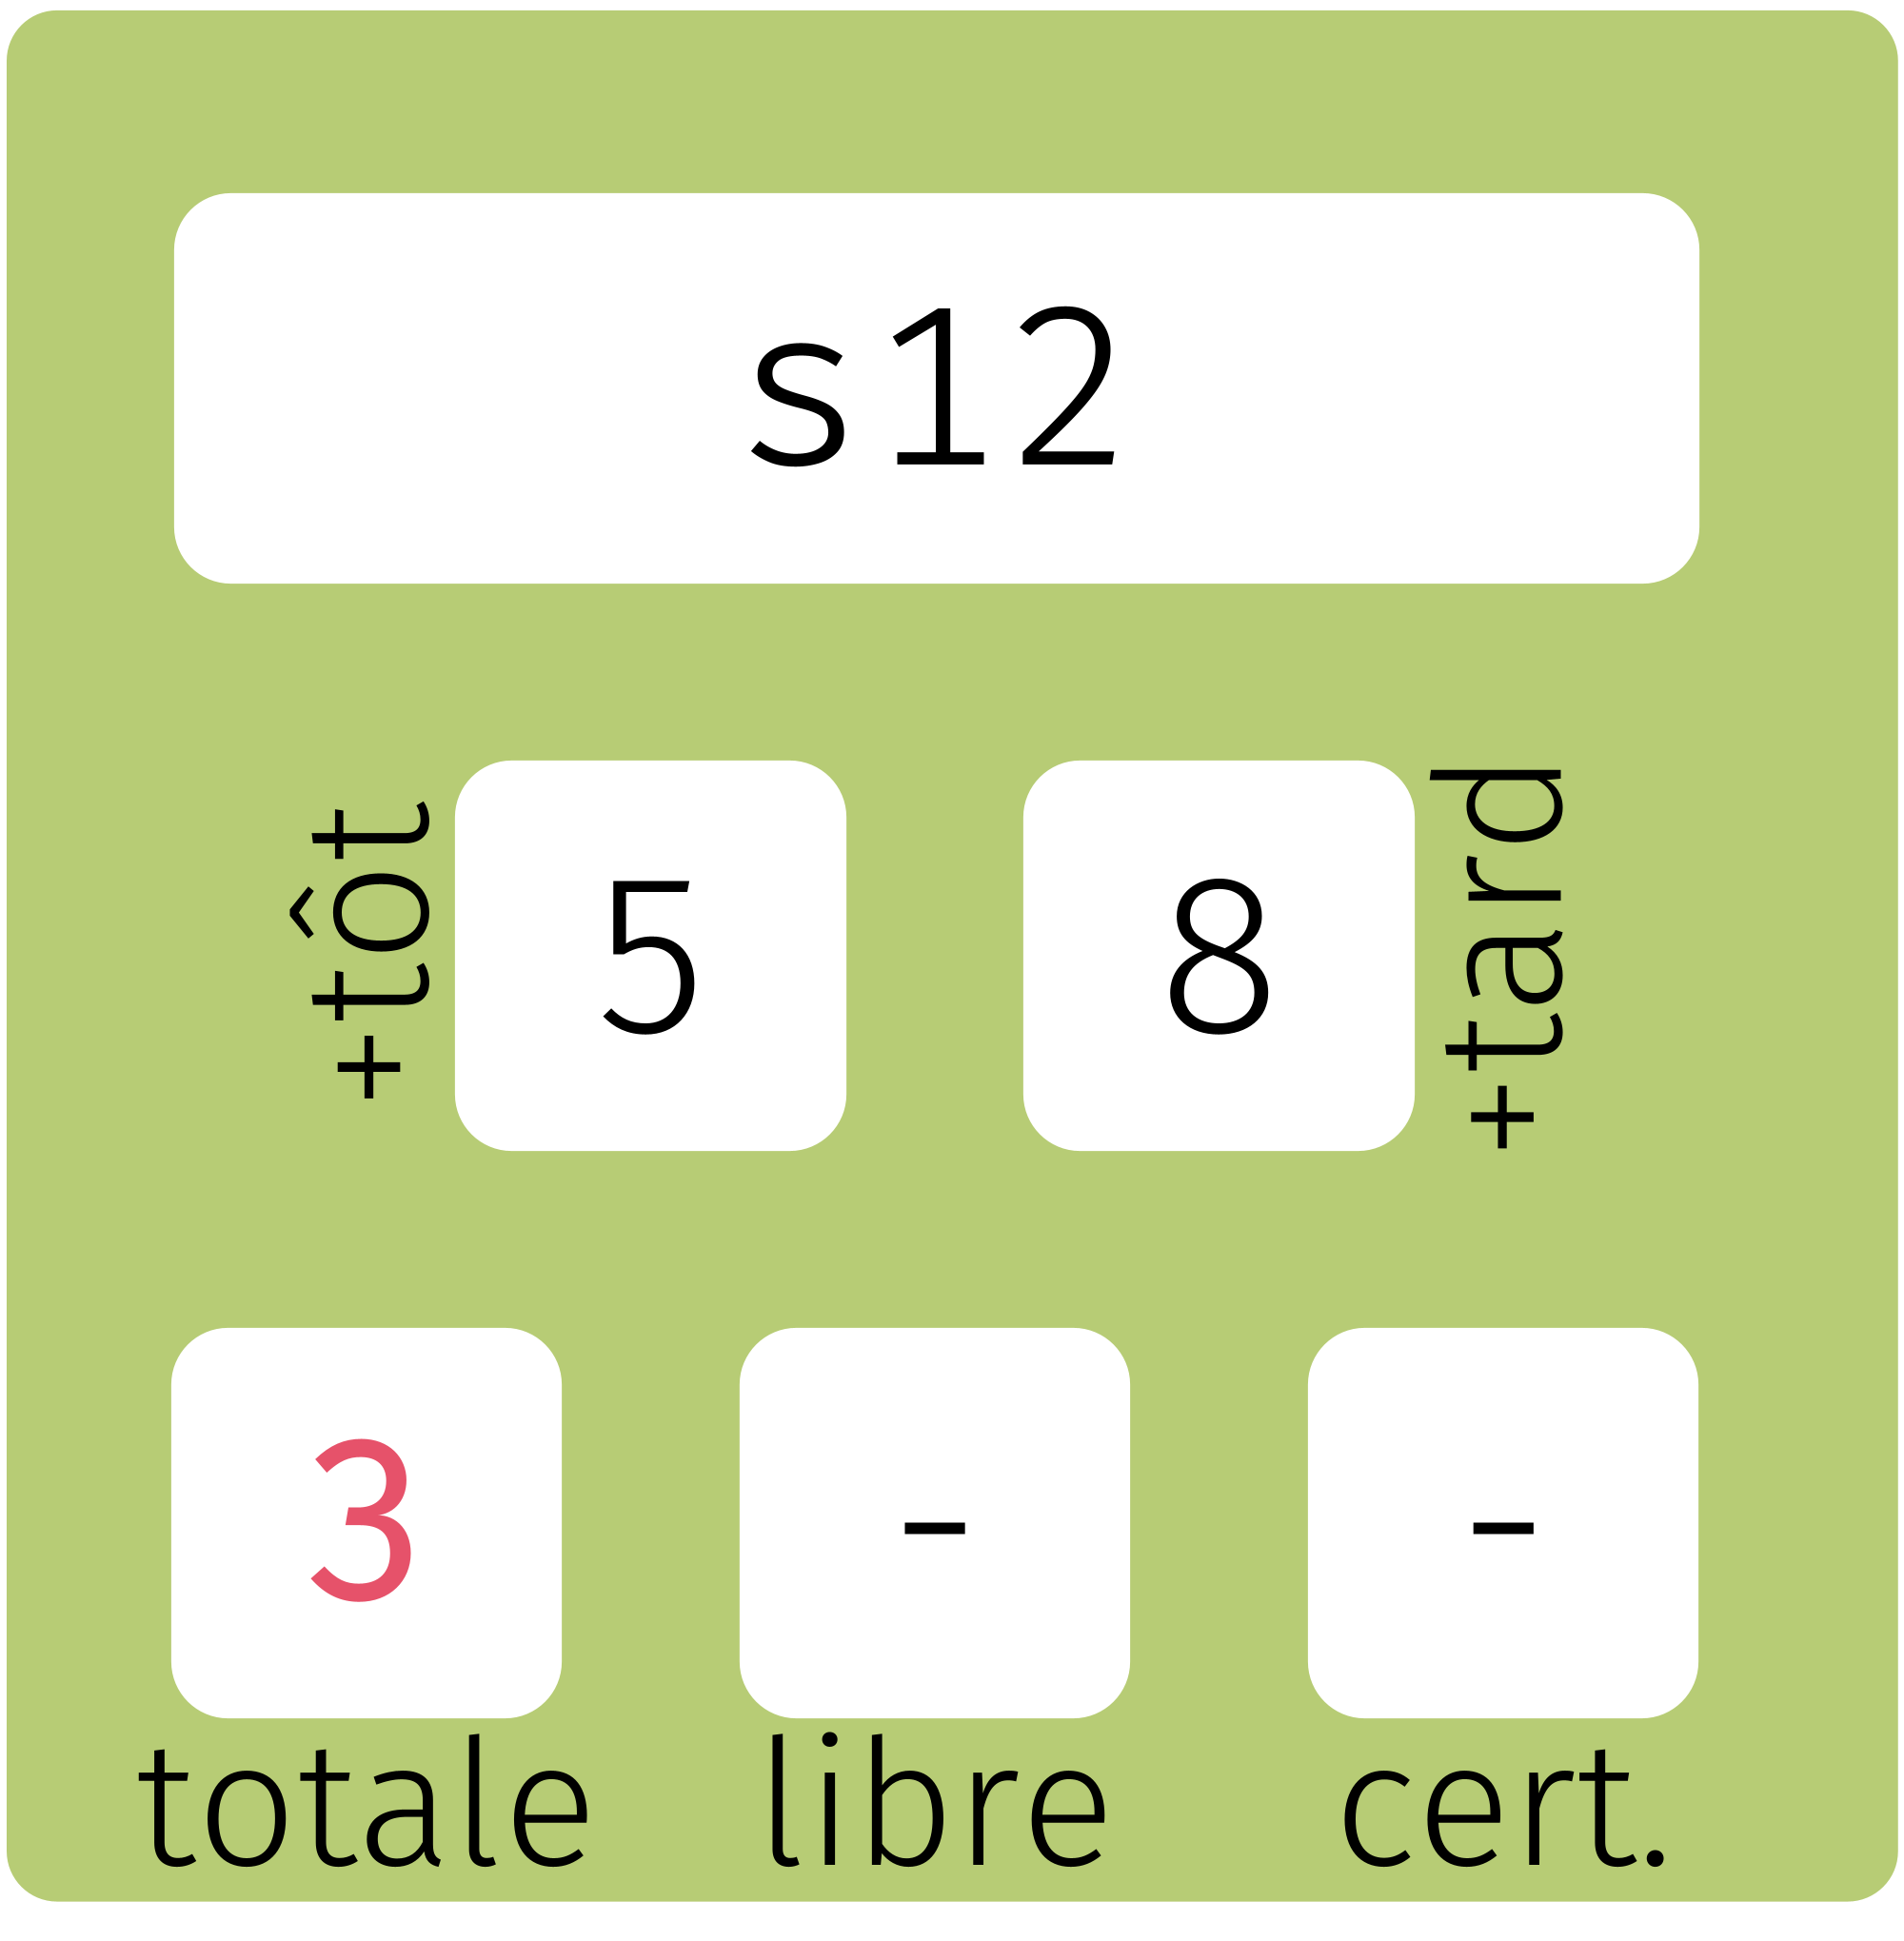
\includegraphics[width=4cm]{graphes2/img/mpm_marge_totale.png}}{La tâche  $s_{12}$ peut commencer au plus tôt au bout de 5 jours et au plus tard au bout de 8 jours. Sa marge totale est donc $MT(s_{12})=3$.\\
        Ce n'est pas une tâche critique : une fois que toutes les tâches antérieures à $s_{12}$ sont effectuées, on peut en théorie encore attendre 3 semaines avant de commencer $s_{12}$.}
\end{exemple}

Calculons les marges totales des tâches de notre projet :

\begin{center}
    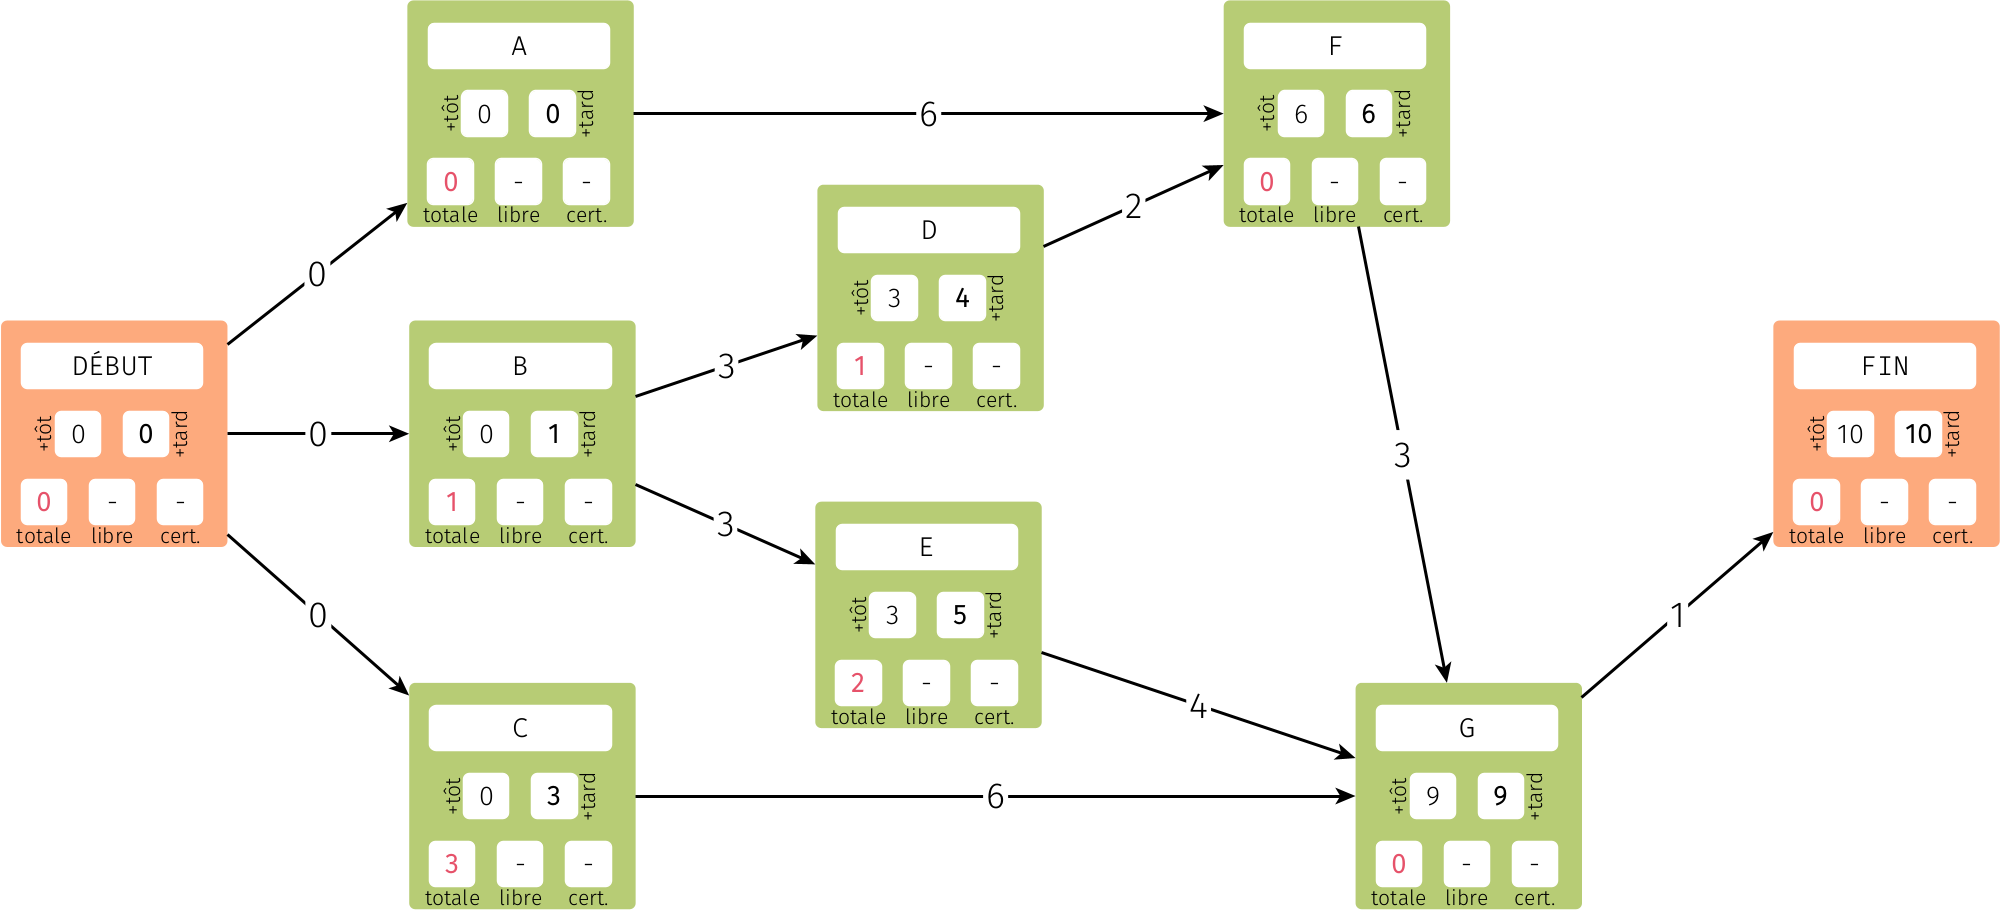
\includegraphics[width=\linewidth]{graphes2/img/exemple_mpm4.png}
\end{center}

Il existe des tâches critiques (en plus du début et de la fin) : A, F et G.

\begin{definition}[ : chemin critique]
    Un chemin critique est un chemin qui n'est composé que de tâches critiques.
\end{definition}

Le chemin début-A-F-G-fin n'est composé que de tâches critiques : c'est un \textit{chemin critique}.

\subsubsection*{Marge libre}

\begin{definition}[ : marge libre]
    La \textit{marge libre} d'une tâche, c'est le retard maximum que l'on peut accepter sur la date de début \textit{au plus tôt} d'une tâche sans que cela ne retarde la date de début \textit{au plus tôt} de chacune des dates suivantes.
    $$ML(s_i)=\min\left(\left\{t(s_j)-t(s_i)-d(s_i)\::\:s_j\,\text{ successeur de }\:s_i\right\}\right)$$
\end{definition}
\begin{exemple}[]
    \begin{center}
        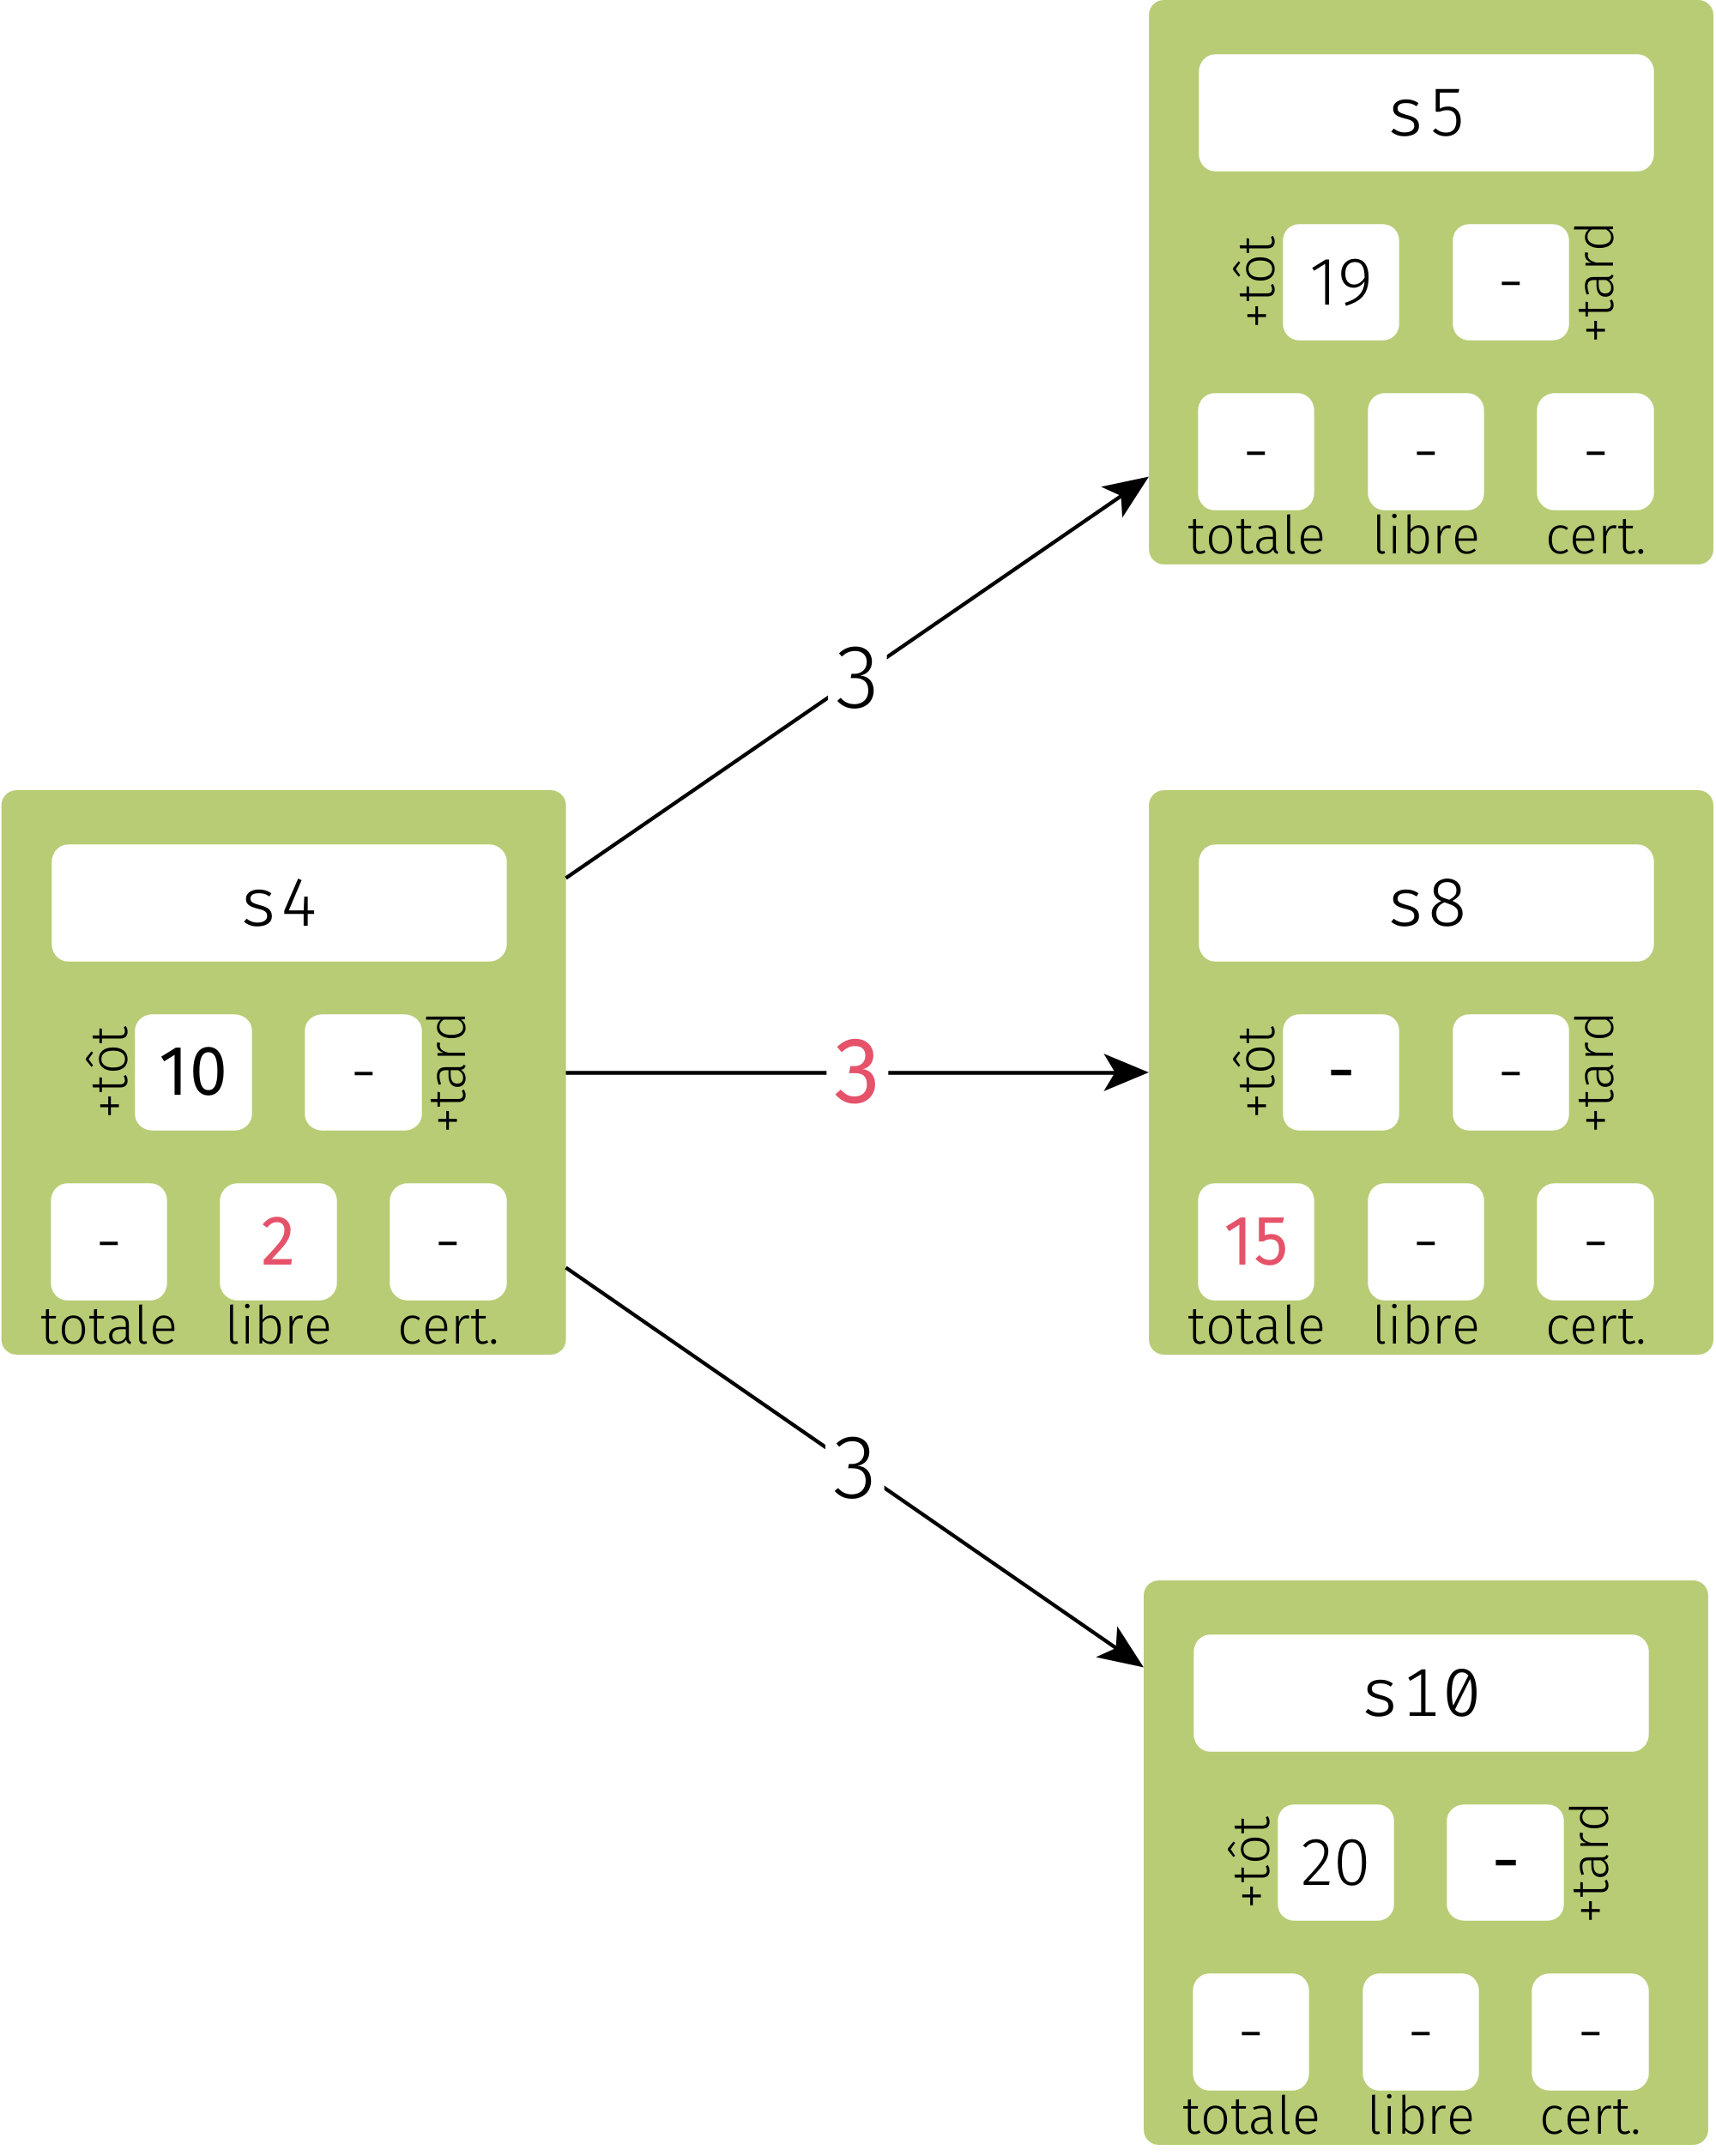
\includegraphics[width=5.5cm]{graphes2/img/mpm_marge_libre.png}
    \end{center}
    La tâche $s_4$ dure trois jours. En la commençant au plus tôt on finit à 13 jours. Il y a des marges pour chacune des tâches suivantes, la plus petite est pour $s_8$ et vaut 3 jours. \\
    Ainsi $ML(s_4)=3$.
\end{exemple}

Calculons les marges libres pour notre exemple :

\begin{center}
    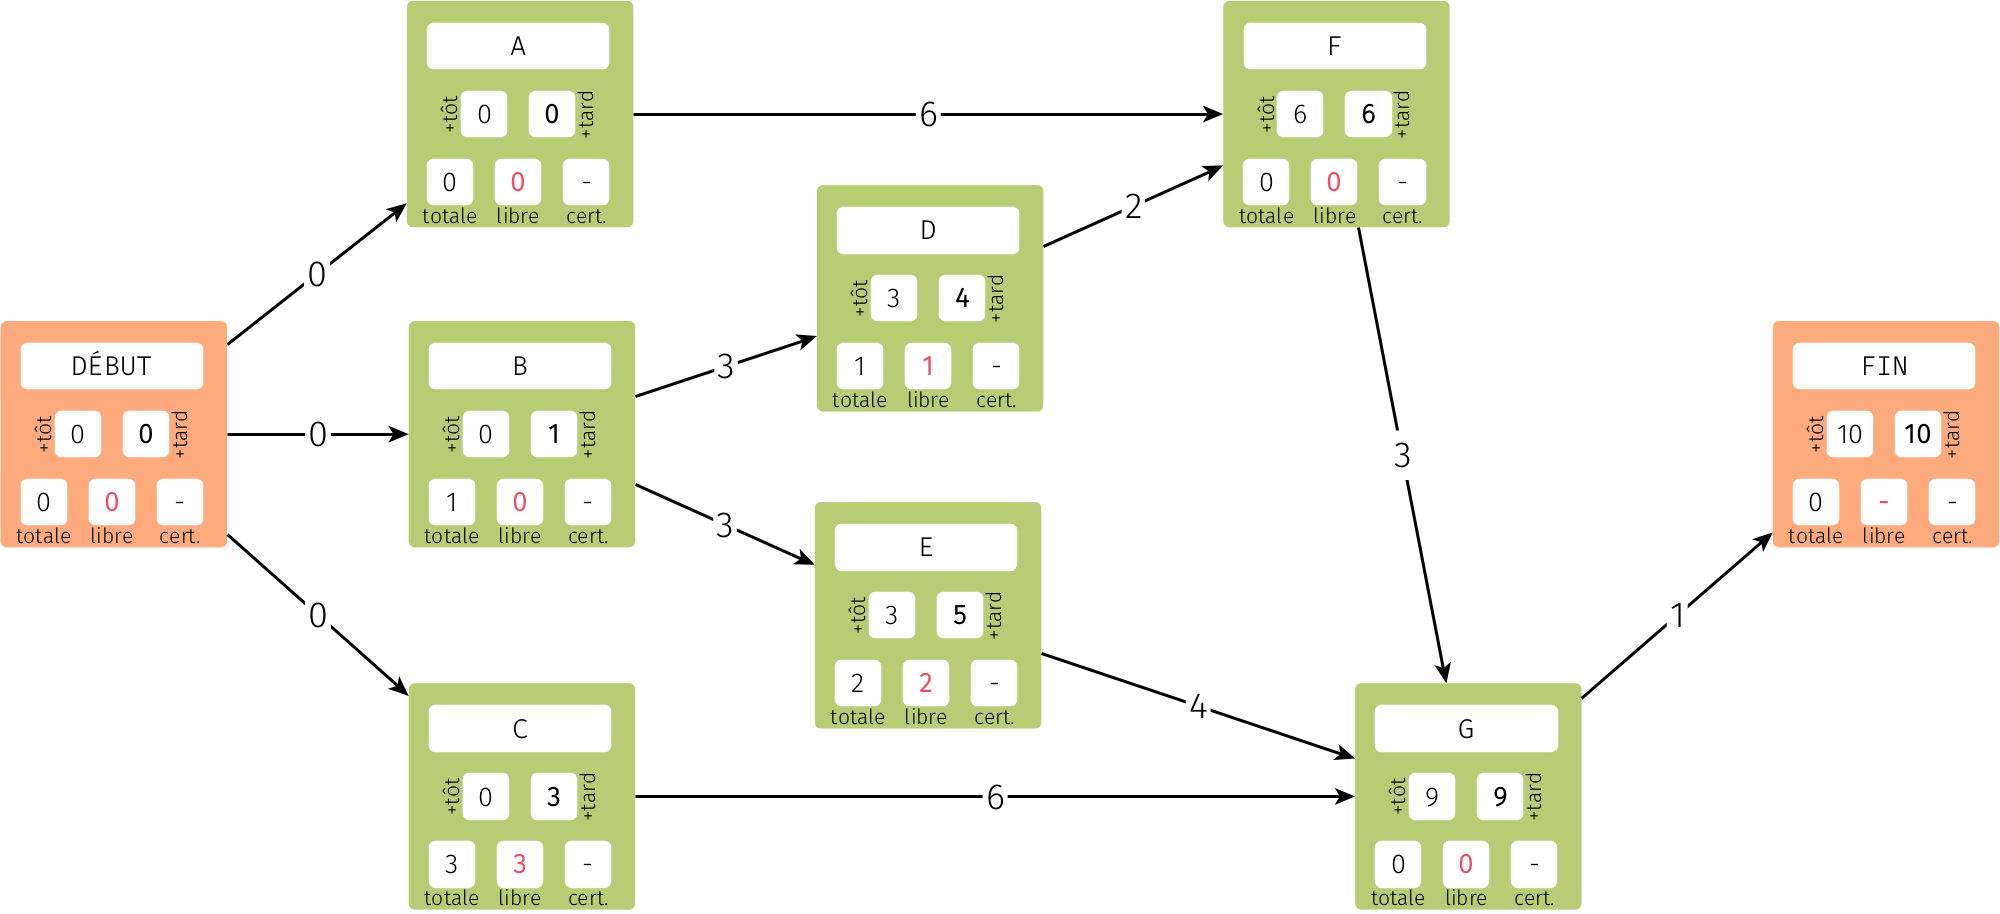
\includegraphics[width=\linewidth]{graphes2/img/exemple_mpm5.png}
\end{center}


\subsubsection*{Marge certaine}

\begin{definition}[ : marge certaine]
    La \textit{marge certaine} d'une tâche est le retard que l’on peut prendre sur cette tâche sans modifier les dates de début au plus tôt des tâches postérieures, tout en sachant que les tâches précédentes ont commencées à leur date au plus tard.

    Il faut commencer par calculer \textit{la date au plus tôt retardée de la tâche}, c'est-à-dire la date au plus tôt de la tâche sachant que les tâches précédentes ont commencé à leur date au plus tard. Pour une tâche $s_i$ cette date est $$DR(s_i)=\max\left(\left\{T(s_j)+d(s_j)\::\:s_j\,\text{ prédécesseur de }\:s_i\right\}\right)$$
    Et alors la marge certaine est
    $$MC(s_i)=\min\left(\left\{t(s_j)-DR(s_i)-d(s_i)\::\:s_j\,\text{ successeur de }\:s_i\right\}\right)$$
    Avec la convention que si ce résultat est négatif on décide que $MC(s_i)=0$.
\end{definition}
\begin{exemple}[]
    \begin{center}
        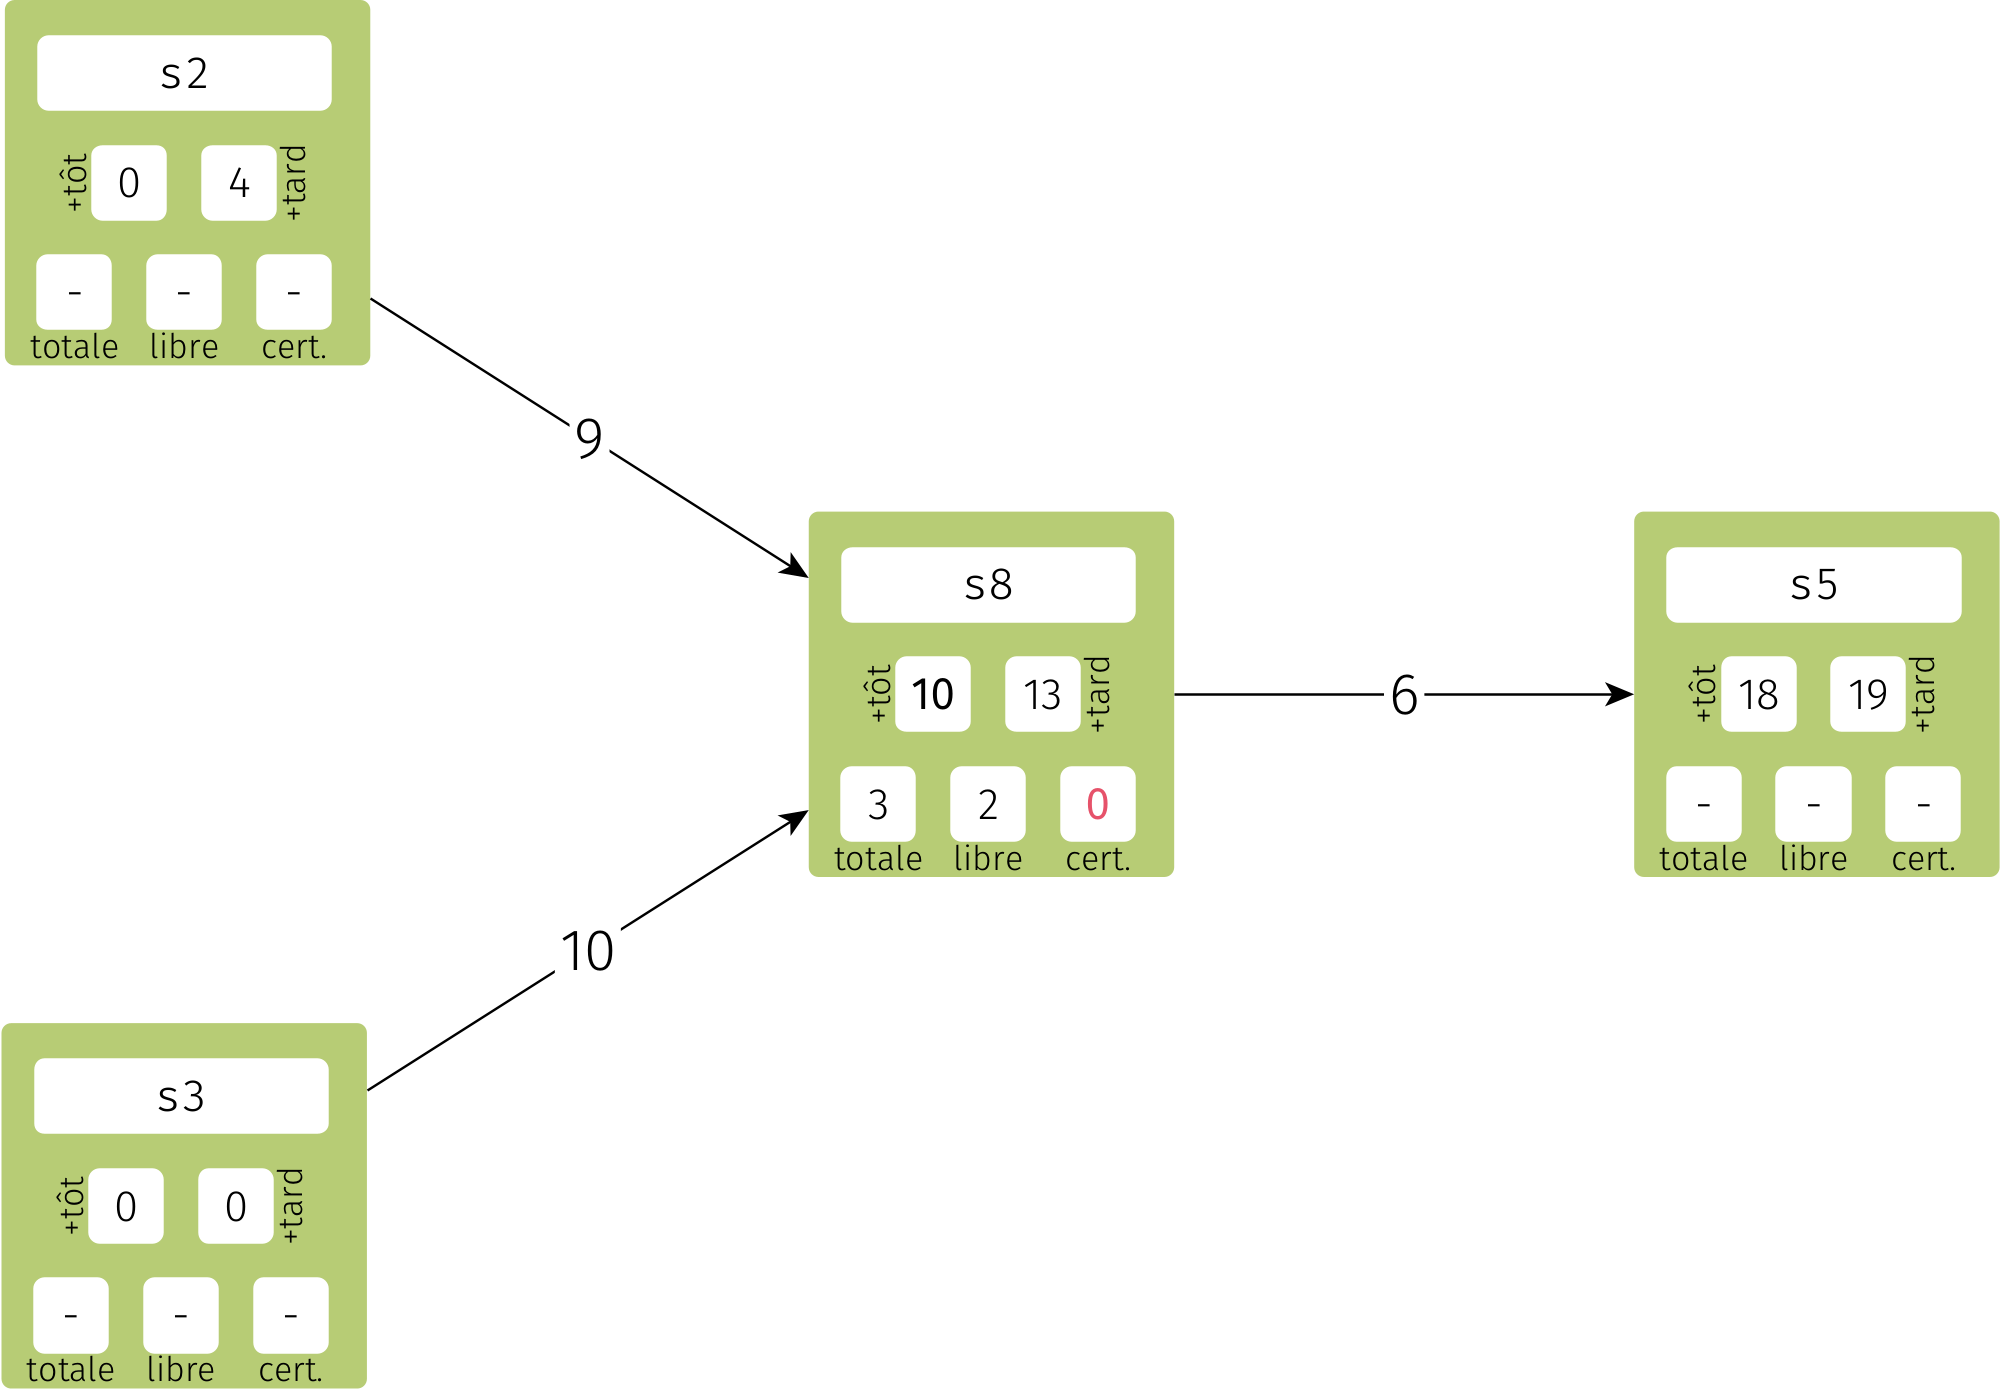
\includegraphics[width=10cm]{graphes2/img/mpm_marge_certaine.png}
    \end{center}
    Pour calculer la marge certaine de la tâche $s_4$:
    \begin{itemize}
        \item 	On calcule $DR(s_4)$ : au pire $s_3$ commence à 0 et dure 10 donc fait commencer $s_4$ à 10, et au pire $s_2$ commence à 9 et dure $4$ donc fait commencer $s_4$ à 13. La date retardée $DR(s_4)$ vaut donc 13.
        \item 	$s_4$ n'a qu'un successeur : $s_5$, on calcule donc $t(s_5)-DR(s_4)-d(s_4)$, cela donne $18-13-6=-1$, c'est négatif donc $MC(s_4)=0$.
    \end{itemize}

\end{exemple}

Calculons les marges certaines pour notre exemple :

\begin{center}
    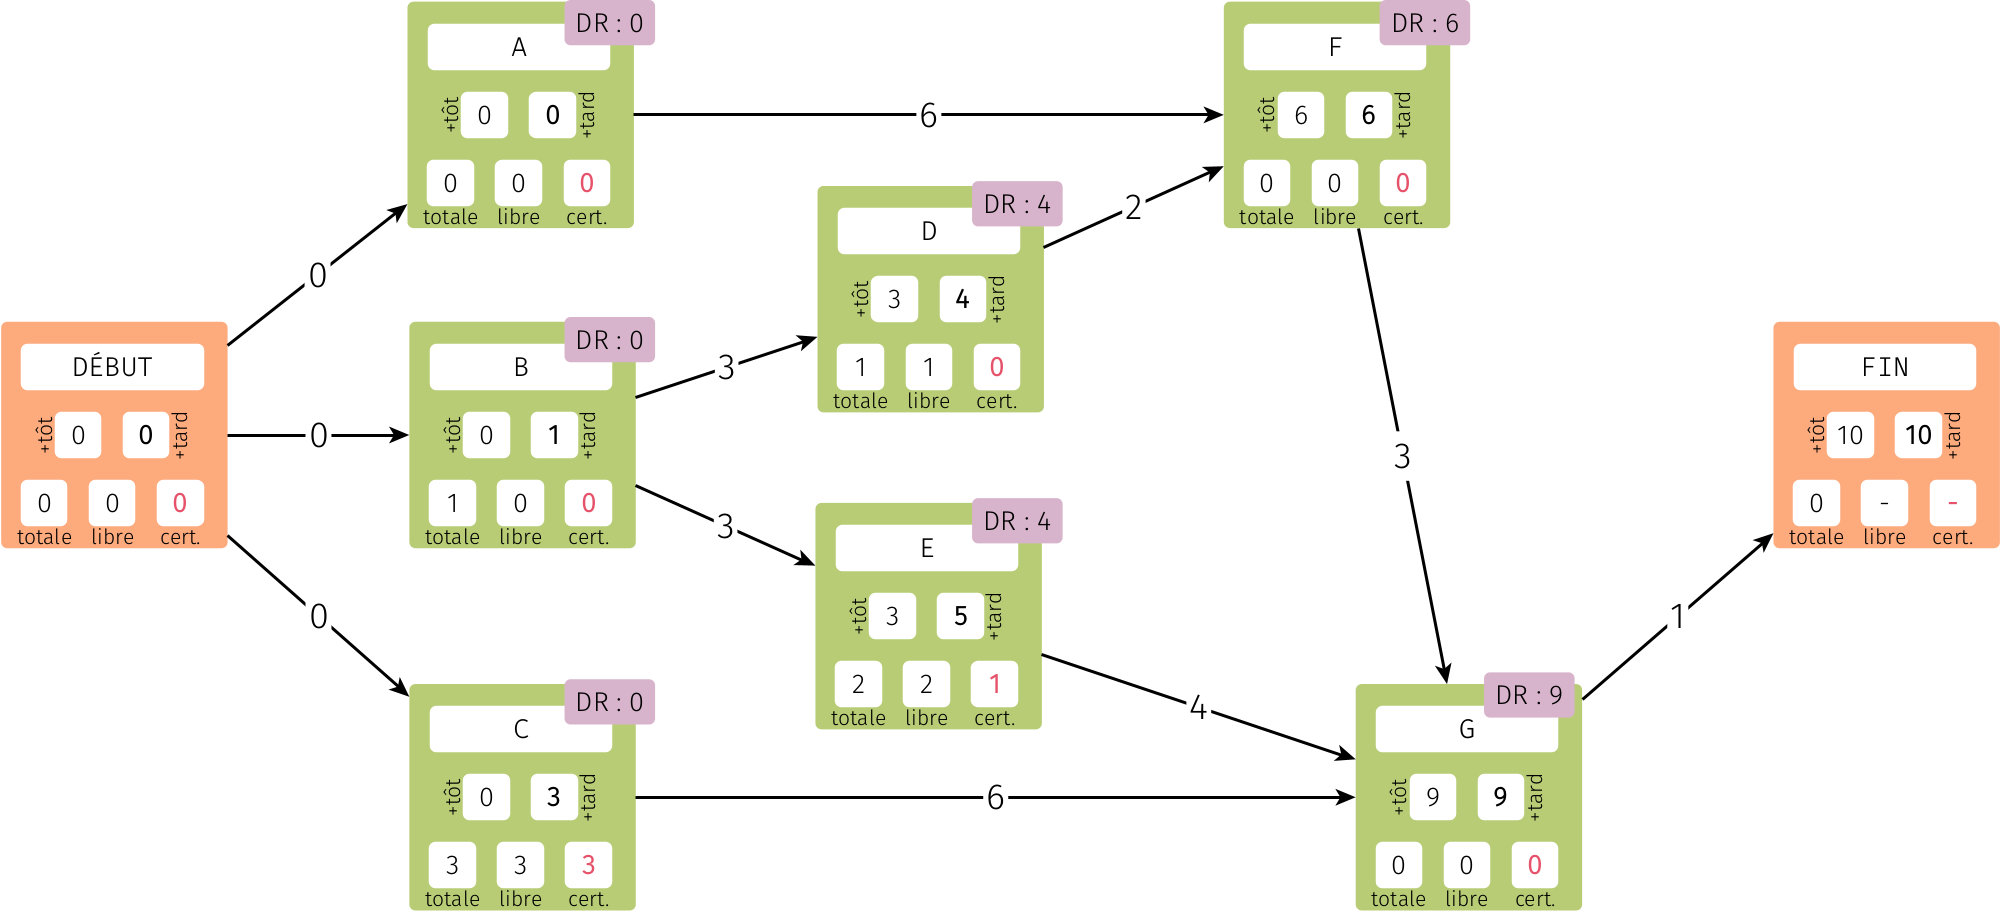
\includegraphics[width=\linewidth]{graphes2/img/exemple_mpm6.png}
\end{center}

L'intérêt de l'ordonnancement est de déterminer les tâches critiques, dont le déroulement devra être rigoureusement suivi pour ne pas perturber la suite du projet. Lorsque des tâches fortement non critiques (comme les tâches C ou E) sont trouvées, on peut par exemple diminuer un peu les ressources attribuées à ces tâches, quitte à utiliser leur marge libre, dans le but de réduire le coût global du projet.

\begin{exercice}[]
    La mise en service d'un nouvel équipement routier demande la réalisation d'un certain nombre de tâches. Le tableau ci-dessous les recense, avec les contraintes d'antériorité.

    \begin{center}
        \tabstyled
        \begin{tabular}{|c|c|c|c|c|c|c|c|}
            \hline
            \ccell Tâches             & A & B & C & D & E & F    & G       \\\hline

            \ccell Durée en jours     & 6 & 3 & 6 & 2 & 4 & 3    & 1       \\\hline
            \ccell Tâches antérieures & - & - & - & B & B & A, D & C, E, F \\\hline
        \end{tabular}
    \end{center}
    \begin{enumerate}
        \item Déterminer le niveau de chacune des tâches.
        \item Construire le graphe d'ordonnancement du projet et calculer les dates au plus tôt et au plus tard de chaque tâche.
        \item Déterminer le chemin critique. Quelle est la durée minimale de réalisation du projet ?
        \item Calculer la marge totale de la tâche E. Quelle est sa signification ?
        \item Calculer la marge libre de C. Quelle est sa signification ?
    \end{enumerate}
\end{exercice}

\begin{exercice}[]
    La réalisation d'un projet nécessite plusieurs tâches dont les duréees en jours et les contraintes d'antériorités sont résumées ci-dessous.
    \begin{center}
        \tabstyled
        \begin{tabular}{|c|c|c|c|c|c|c|c|c|c|c|}
            \hline
            \ccell Tâches             & A & B & C & D & E    & F & G    & H    & I & J    \\\hline
            \ccell Durée en jours     & 4 & 2 & 2 & 1 & 2    & 5 & 3    & 3    & 3 & 4    \\\hline
            \ccell Tâches antérieures & - & - & A & A & A, B & C & D, E & E, G & H & F, I \\\hline
        \end{tabular}
    \end{center}
    \begin{enumerate}
        \item Déterminer le niveau de chaque tâche.
        \item Construire le graphe d'ordonnancement du projet et calculer les dates au plus tôt et au plus tard de chaque tâche.
        \item Déterminer le chemin critique. Quelle est la durée minimale de réalisation du projet ?
        \item En réalité, la tâche C a nécessité une durée de 5 jours. Est-ce que cela a eu une incidence sur la durée de réalisation du projet ?
    \end{enumerate}
\end{exercice}
